%  ========================================================================
%  Copyright (c) 1985-2014 The University of Washington
%
%  Licensed under the Apache License, Version 2.0 (the "License");
%  you may not use this file except in compliance with the License.
%  You may obtain a copy of the License at
%
%      http://www.apache.org/licenses/LICENSE-2.0
%
%  Unless required by applicable law or agreed to in writing, software
%  distributed under the License is distributed on an "AS IS" BASIS,
%  WITHOUT WARRANTIES OR CONDITIONS OF ANY KIND, either express or implied.
%  See the License for the specific language governing permissions and
%  limitations under the License.
%  ========================================================================
%

% Documentation for University of Washington thesis LaTeX document class
% by Jim Fox
% fox@washington.edu
%
%    Revised for version 2015/03/03 of uwthesis.cls
%
%    This document is contained in a single file ONLY because
%    I wanted to be able to distribute it easily.  A real thesis ought
%    to be contained on many files (e.g., one for each chapter, at least).
%
%    To help you identify the files and sections in this large file
%    I use the string '==========' to identify new files.
%
%    To help you ignore the unusual things I do with this sample document
%    I try to use the notation
%       
%    % --- sample stuff only -----
%    special stuff for my document, but you don't need it in your thesis
%    % --- end-of-sample-stuff ---


%    Printed in twoside style now that that's allowed
%
 
\documentclass [11pt, proquest] {/Users/jgruszko/Documents/Thesis/Template/uwthesis}[2015/03/03]

\usepackage{graphicx}
\usepackage{amsmath}
 \usepackage{caption}
 \usepackage{subcaption}
 \captionsetup{compatibility=false}
%
% The following line would print the thesis in a postscript font 

% \usepackage{natbib}
% \def\bibpreamble{\protect\addcontentsline{toc}{chapter}{Bibliography}}

\setcounter{tocdepth}{1}  % Print the chapter and sections to the toc
 

% ==========   Local defs and mods
%
\usepackage{lineno}
\usepackage{longtable}  
\usepackage{url}
\usepackage{hyperref}
\usepackage{graphicx}
\usepackage{amsmath,amssymb,bbold,bm}
\usepackage{epstopdf}
\usepackage{xcolor}
\usepackage{lipsum}
\usepackage{gensymb}
\definecolor{blue}{RGB}{50,0,255} 	
\colorlet{blueh}{blue!30}
\usepackage{fancyhdr}
\usepackage{afterpage}
\usepackage{siunitx}
\usepackage{booktabs}
\usepackage{subcaption}
\usepackage{physics}
\usepackage{rotating}
\usepackage{xr}

\externaldocument{Ch1}
\externaldocument{Ch2}
\externaldocument{Ch3}
\externaldocument{Ch5}
\externaldocument{Ch6}

% ==========   Local defs and mods
%

% --- sample stuff only -----
% These format the sample code in this document

\usepackage{alltt}  % 
\newenvironment{demo}
  {\begin{alltt}\leftskip3em
     \def\\{\ttfamily\char`\\}%
     \def\{{\ttfamily\char`\{}%
     \def\}{\ttfamily\char`\}}}
  {\end{alltt}}
 
  % Definitions and macros
\newcommand{\degrees}{$^{\circ}$}                                         % makes a correct degree symbol
\newcommand{\cpp}{C\protect\raisebox{.25ex}{++}\ }               % formats C++ correctly
\newcommand{\MJ}{M{\footnotesize AJORANA}}                        % this works for bolding in titles and the toc
\newcommand{\MJDemo}{D{\footnotesize EMON\-STRAT\-OR}} 	% this works for bolding in titles and the toc
\newcommand{\snop}{SNO\protect\raisebox{.25ex}{+}}             % formats SNO+ nicely
\newcommand{\nonubb}  {${0 \nu \beta \beta}$}                       % neutrinoless double beta decay in math mode
\newcommand{\iso}[2]{$^{#1}$#2}                                        % Makes a properly formatted isotope symbol e.g. \iso{28}{Si}

% metafont font.  If logo not available, use the second form
%
% \font\mffont=logosl10 scaled\magstep1
\let\mffont=\sf
% --- end-of-sample-stuff ---
  
\def\ppc{P-PC}  
\def\MJ{{\sc Majorana}}             %Majorana project name
\def\DEM{{\sc Demonstrator}}             %Demonstrator in small caps
\def\thttt{$^{232}\mathrm{Th}$}
\def\thtte{$^{228}\mathrm{Th}$}
\def\utte{$^{238}\mathrm{U}$}
\def\am{$^{241}\mathrm{Am}$}
\def\po{$^{210}\mathrm{Po}$}
\def\nonubb{$\beta\beta(0\nu)$}
\def\twonubb{$\beta\beta(2\nu)$}


\begin{document}
 
% ==========   Preliminary pages
\prelimpages
 
%
% ----- copyright and title pages
%
\Title{Surface Alpha Interactions in P-Type Point-Contact HPGe Detectors: Maximizing Sensitivity of $^{76}$Ge Neutrinoless Double-Beta Decay Searches}
\Author{Julieta Gruszko}
\Year{2017}
\Program{UW Physics}

\Chair{Jason Detwiler}{Assistant Professor}{Physics}
\Signature{Ann Nelson}
\Signature{Grey Rybka}

\copyrightpage

 \titlepage  

%
% ----- signature and quoteslip are gone
%

%
% ----- abstract
%


\setcounter{page}{-1}
\abstract{
Though the existence of neutrino oscillations proves that neutrinos must have non-zero mass, Beyond-the-Standard-Model physics is needed to explain the origins of that mass. One intriguing possibility is that neutrinos are Majorana particles, i.e., they are their own anti-particles. Such a mechanism could naturally explain the observed smallness of the neutrino masses, and would have consequences that go far beyond neutrino physics, with implications for Grand Unification and leptogenesis. 

If neutrinos are Majorana particles, they could undergo neutrinoless double-beta decay (\nonubb), a hypothesized rare decay in which two antineutrinos annihilate one another. This process, if it exists, would be exceedingly rare, with a half-life over $10^{25}$ years. Therefore, searching for it requires experiments with extremely low background rates. One promising technique in the search for \nonubb\ is the use of P-type point-contact (\ppc) high-purity Germanium (HPGe) detectors enriched in $^{76}$Ge, operated in large low-background arrays. This approach is used, with some key differences, by the \MJ\ and GERDA Collaborations. 

A problematic background in such large granular detector arrays is posed by alpha particles incident on the surfaces of the detectors, often caused by $^{222}$Rn contamination of parts or of the detectors themselves. In the \textsc{Majorana Demonstrator}, events have been observed that are consistent with energy-degraded alphas originating near the passivated surface of the detectors, leading to a potential background contribution in the region-of-interest for neutrinoless double-beta decay. However, it is also observed that when energy deposition occurs very close to the passivated surface, high charge trapping occurs along with subsequent slow charge re-release. This leads to both a reduced prompt signal and a measurable change in slope of the tail of a recorded pulse. Here we discuss the characteristics of these events and the development of a filter that can identify the occurrence of this delayed charge recovery (DCR) effect, allowing for the efficient rejection of passivated surface alpha events in analysis. 

Using a dedicated test-stand called the TUM Upside-down BEGe (TUBE) scanner, we have characterized the response of a \ppc\ detector like those used in the \DEM\ to alphas incident on the sensitive surfaces, developing a model for the radial dependence of the energy loss to charge trapping and determining the dominant mechanism behind the delayed charge effect. We have also used these measurements to demonstrate the complementarity of the DCR analysis with the drift-time analysis that is used to identify alpha background candidate events in the GERDA detectors. Using these two methods, we demonstrate the ability to effectively reject all alpha events (to within statistical uncertainty) with only 0.2\% bulk event sacrifice. 

Applying the DCR analysis to the events observed in the \MJ\ \DEM, we find that it reduces the backgrounds in the \nonubb\ region-of-interest by a factor of 31, increasing the expected experimental sensitivity by a factor of 3 over the lifetime of the \DEM. The results of the dedicated measurements in the TUBE scanner can be used to build a background model for alpha decays in the \DEM ; here, we examine two simplified geometric models for the alpha source distribution and find that the observed spectral shape is consistent with alpha events originating in the plastics of the detector units. 
 }
%
% ----- contents & etc.
%
\tableofcontents
\listoffigures
\listoftables  % I have no tables
 
%
% ----- glossary 
%
\chapter*{Glossary}      % starred form omits the `chapter x'
\addcontentsline{toc}{chapter}{Glossary}
\thispagestyle{plain}
%
\begin{glossary}
\item[MJD] The \MJ\ \MJDemo\ 
\item[HPGe] High-purity Germanium
\item[PPC] P-type point contact detector.
\end{glossary}

% ==========      Text pages
%

\textpages
 
% ========== Chapter 1
% ========== Chapter 1
 
\chapter {Neutrino Physics and \nonubb Introduction}
\section{Neutrinos as a Key to New Physics}
\subsection{The ``Desperate Remedy"}
Since its introduction by Wolfgang Pauli in 1930, the neutrino has been allowing physicists to reconcile theories and experiments that did not quite align. At the time, the theories in question were the conservation of energy and angular momentum; beta decay observations seemed to violate these key principles. Instead of carrying away the full Q-value of the decay, the observed electrons could carry off a range of energies up to that value. And instead of going off back-to-back, as expected in a two-body decay under momentum conservation laws, the recoiling nucleus and electron could have any angle between them. 

As a ``desperate remedy," Pauli proposed the neutrino \cite{Pauli1930}-- a light, neutral particle that was being created in the decay, carrying off the missing energy and momentum. If it did not interact via the strong or electromagnetic forces, such a particle would easily escape most detectors. In fact, the elusive neutrino escaped detection for over twenty years, until it was eventually observed in 1956 \cite{Cowan1956}. With the addition of this particle to the standard model, beta decay was explained as a three-body process, and the conservation laws were saved.

\subsection{The Solar Neutrino Problem}
Along with the neutrino, the concepts of lepton number and lepton number conservation were introduced. This value, in the standard model, is conserved in weak interactions, which proceed via two classes of vertex, called the neutral and charged currents. The Feynman diagrams for these processes are seen in Fig.~\ref{weak_diagrams}. In the charged current interactions, a charged lepton (i.e. the electron, muon, or tau, or their antiparticles) participates in the interaction, and the (anti-)neutrino always occurs with the W+(-) boson. In the neutral current interaction, a lepton and its corresponding anti-lepton always participate along with the Z boson. 

\begin{figure}[h]
\hfil 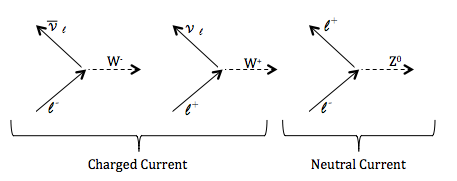
\includegraphics[width = .80\textwidth]{/Users/jgruszko/Documents/Thesis/Images/Ch1/WeakDiagrams.png} \hfil
\caption{The primitive vertices of the Feynman diagrams for weak interactions between leptons in the standard model. Equivalent vertices exist for the quarks. \cite{PDG2014}}
\label{weak_diagrams}
\end{figure}

There are (at least) three neutrino flavors, corresponding to the three charged leptons, which form a basis of flavor eigenstates. They are created in these eigenstates-- in a charged current interaction emitting an electron, for instance, the standard model requires that an electron anti-neutrino is also created. Originally, it was believed that neutrinos also followed lepton-flavor conservation. Since in the standard model, neutrinos are massless, that electron anti-neutrino would propagate in its flavor eigenstate, and remain an electron anti-neutrino. 

With this assumption firmly in place, physicists began to attempt to detect the neutrinos created in the sun. Based on astrophysical models of solar fusion processes \cite{Bahcall}, 7E10 $\nu_{e}$/cm$^2$/s were expected to reach earth. When Ray Davis measured the solar neutrino flux in the Homestake experiment, however, he found far fewer $\nu_{e}$, about a third the flux that Bahcall's model predicted. Later experiments confirmed this low $\nu_{e}$ flux -- once again the theory (this time the theory behind fusion models of the sun) and the experiments did not agree.

As in the 1930s, the unexpected physics of the neutrino `saved the day.' If the neutrino was not massless, as the Standard Model seemed to assert, but instead had a small mass, it would not propagate in its flavor eigenstate. Instead it would propagate in a mass eigenstate, and if these eigenstates were not equivalent, it would change from one flavor to another as it traveled from the sun to detectors on earth. 

Testing this theory required detectors that could measure the total neutrino flux, instead of just the flux of electron-flavor neutrinos. With the construction of Super-Kamiokande and SNO, the total neutrino flux was measured in 2001, and neutrino oscillations were seen. The mixing of the mass eigenstates in a given flavor eigenstate is described by the PMNS matrix, 
\[
\begin{bmatrix}
\nu_e\\
\nu_\mu\\
\nu_\tau\\
\end{bmatrix}
=
\begin{bmatrix}
U_{e1} & U_{e2} & U_{e3} \\ 
U_{\mu1} & U_{\mu2} & U_{\mu3} \\ 
U_{\tau1} & U_{\mu2} & U_{\mu3} \\ 
\end{bmatrix}
\begin{bmatrix}
\nu_1\\
\nu_2\\
\nu_3\\
\end{bmatrix}
\]

Unlike the quarks, neutrino

- Focus on oscillation, expand this paragraph:
As the properties of neutrinos become better understood, they continue to play this role, pulling our theories back from the brink of incorrectness-- the ``solar neutrino problem" was eventually resolved by the introduction of neutrino flavor oscillations and neutrino mass. \cite{PDG2014} Other proposed aspects of neutrino physics could reveal neutrinoless double beta decay, a lepton number-violating process that could explain the source of matter/anti-matter imbalance in the universe. If this decay were observed, the neutrino would be a Majorana particle (meaning that it is its own antiparticle), explaining the origin and smallness of the neutrino masses.

\subsection{Role of neutrinos in the standard model} 
The neutrinos are standard-model fermions that interact only via gravity and the weak force. 

The weak interaction 


Neutrino oscillation arises because the neutrinos have mass eigenstates (called 1, 2, and 3) that are different from their flavor eigenstates. Therefore, as they propagate in mass/momentum eigenstates, their flavors change according to the PMNS mixing matrix, a unitary matrix that connects the two bases.  The differences in the masses squared of the states also appears in the oscillation probabilities, so these values can be found from neutrino oscillation experiments. The sign of m$_{2,3}$$^{2}$, however, is currently unknown, leading to what are called the ``normal" and ``inverted" cases of the neutrino mass hierarchy, as seen in Fig.~\ref{mass_hierarchy}. 

\begin{figure}[]
\hfil 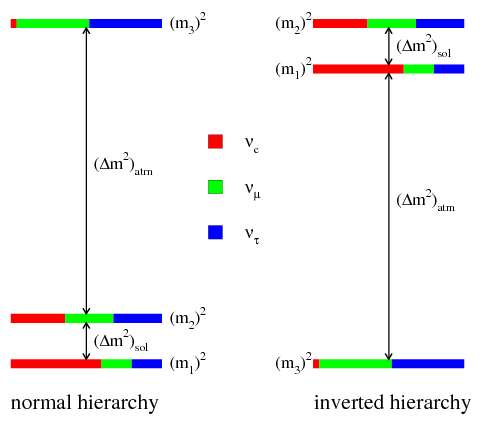
\includegraphics[width = .40\textwidth]{/Users/jgruszko/Documents/Thesis/Images/Ch1/MassHierarchy.png} \hfil
\caption{The two possible cases of the neutrino mass hierarchy \cite{Hewett2012}}
\label{mass_hierarchy}
\end{figure}

	- chirality, helicity, weyl spinors, 
\subsection{Mass mechanisms (Dirac and Majorana)} 
	- why both are problematic
\subsection{Outstanding problems in neutrino physics}
	- Unknown SM neutrino properties (mass, mass hierarchy), sterile neutrinos
         - Neutrino mass-scale problem

Additionally, the overall neutrino mass is not known. The lowest limits, derived from the shape of the $^{3}$He $\beta$-decay spectrum, give $m_{\bar{\nu}_{e}} < 2.3~eV$ \cite{Eitel2005}. More stringent limits, below $0.23~eV$, have been derived from cosmic microwave background observations \cite{PlanckXVI_2013}, but these values are highly model-dependent. The KATRIN experiment plans to directly probe masses down to $m_{\bar{\nu}_{e}} \sim 0.20~eV$ \cite{KATRIN2015}

\subsection{The Neutrino- Majorana or Dirac?}
Because neutrino oscillations have been observed, it is clear that neutrinos have non-zero mass. Minimalistic Higgs models, however, require fine-tuning, unnaturally leaving the neutrino mass about six orders of magnitude smaller than the masses of the other standard model particles. Any mechanism for neutrino mass that avoids this unnaturalness must come from an extension to the standard model. One possibility, called the ``see-saw mechanism," relies on the addition of a Majorana mass term \cite{Supergravity1979}. With the introduction of this term, there are no longer (non-interacting) right-handed neutrinos and left-handed antineutrinos. Instead, the neutrino and antineutrino are opposite-helicity states of the same Majorana particle. The Majorana mass term would contribute to the overall observed neutrino mass along with remaining Dirac mass terms, and could lead to lepton-number violating interactions. These interactions also allow a mechanism by which baryogenesis could be possible, leading to matter/anti-matter imbalance in the observable universe. \cite{DiBari2012}  


	- Nature of neutrino mass
	- Matter asymm, Seesaw mechanism

\section{Double beta-decay introduction}
\subsection{2nBB}
- 0nBB
	
\subsection{Neutrinoless Double Beta Decay}
The most promising process by which to discover the nature of the neutrino is neutrinoless double beta decay. In standard-model two neutrino double-beta decay, a nucleus that contains an even number of nucleons is energetically forbidden from decaying via single beta-decay. Instead, two beta decays occur, leading to the emission of two electrons and two electron anti-neutrinos. In the neutrinoless version of this process the anti-neutrino is exchanged as a virtual particle-- it functions as an outgoing antineutrino for one of the beta decays, and as an incoming neutrino for the other decay. Thus, no neutrinos are seen in the final state:
$$M(A, Z) \rightarrow D(A, Z+2) + 2 e^{-},$$
 and all of the energy of the decay is carried by the electrons. Due to momentum conservation, the nucleons carry a negligible amount of the energy. This decay relies on the non-conservation of lepton number, which is allowed in the Standard Model, though it has not yet been observed, on the Majorana nature of the neutrino, and on the fact that the neutrino is in a mixed helicity state. Because of the last consideration, the effective size of the Majorana mass term, 
 $$\langle m_{\beta\beta} \rangle = |\sum\limits_{i=1}^3 U^2_{ei}m_i|,$$
 where $U_{ei}$ is the mixture of neutrino mass eigenstates $i$ in the electron neutrino, appears in the $0\nu\beta\beta$ rate:
 $$(T_{1/2}^{0\nu})^{-1} = G^{0\nu}|M_{0\nu}|^{2}\left(\frac{\langle m_{\beta\beta} \rangle}{m_e}\right)^2 .$$
 $G^{0\nu}$ is a phase space factor, $M_{0\nu}$ is the nuclear matrix element, and $m_e$ is the electron mass. Because they contribute to $m_{\beta\beta}$, both the overall neutrino mass and the mass hierarchy can contribute to the observed rate, as seen in Fig.~\ref{0nBBrate}. The experimental signature of such a decay would be a delta-peak in energy at the endpoint of the two-neutrino mode spectrum, as in Fig.~\ref{0nBBspectrum}.
 
 \begin{figure}[h]
 \centering
    \begin{subfigure}[b]{.40\textwidth}
      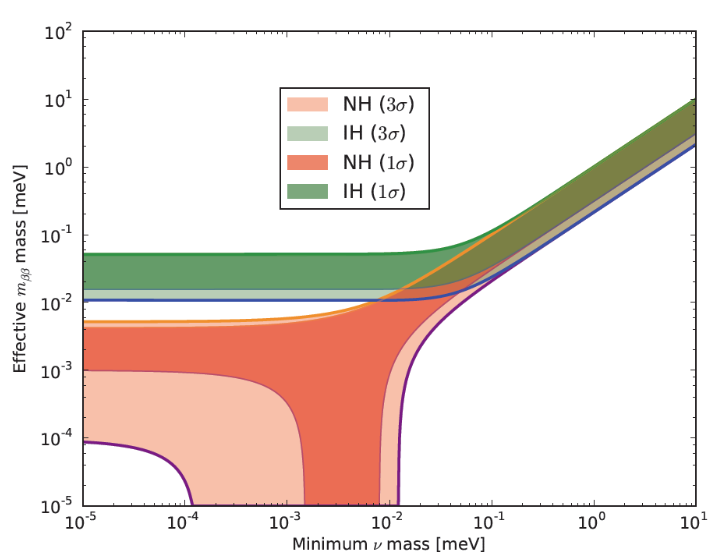
\includegraphics[width =\textwidth]{/Users/jgruszko/Documents/Thesis/Plots/Ch1/0nBB_Rate.png}
       \caption{$m_{\beta\beta}$, and therefore the $0\nu\beta\beta$ rate, depend on the neutrino mass hierarchy and the overall mass scale \cite{ZuberINT2015} .}
        \label{0nBBrate}
        \end{subfigure}   
         \hfil
        \begin{subfigure}[b]{0.4\textwidth}
      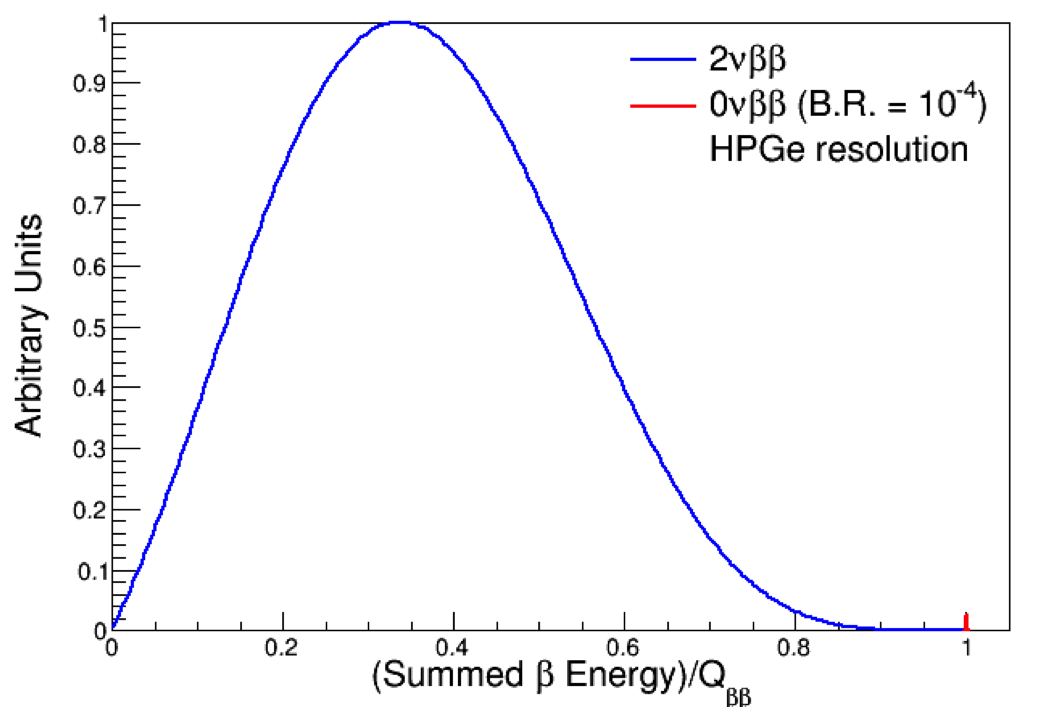
\includegraphics[width =\textwidth]{/Users/jgruszko/Documents/Thesis/Plots/Ch1/DoubleBetaEnergy.png} 
      \caption{The experimental signature of $0\nu\beta\beta$ decay as it would appear in \iso{76}{Ge}. Plot courtesy of Jason Detwiler.}
      \label{0nBBspectrum}
    \end{subfigure}   
\end{figure}
 

	- Neutrino mass dependence
- Potential implications of 0nBB
\section{Measuring \nonubb}
- Experimental requirements
\subsubsection{Observing 0$\nu\beta\beta$}
Current limits set the $0\nu\beta\beta$ half-life to greater than $10^{25}$ years \cite{EXO2014}. To observe such a rare decay, backgrounds of $0\nu\beta\beta$ experiments must be extremely low, and the mass of source material must be as large as possible. Several strategies are commonly used by the $0\nu\beta\beta$ community. 

Some are determined solely by the choice of source material:
\begin{itemize}
\item Choice of Q Value: The higher the Q-value of the $0\nu\beta\beta$ decay in some material, the less background contamination will occur in the signal region. While incomplete energy collection, Compton scattering, and other processes can cause background events to appear at energies below the peak value of the decay, events generally cannot gain energy by any process. 
\item Enrichment: Source materials often have to be enriched in the $0\nu\beta\beta$ isotope to allow for higher source masses without increasing backgrounds. The ease and expense of this process varies widely depending on the material, as does the need for enrichment.
\item Favorable Matrix Elements: $M_{0\nu}$ varies between isotopes; a favorable rate could increase the $0\nu\beta\beta$ rate. However, different calculation strategies lead to variation in these values that is on the order of the difference between isotopes. See \cite{Simkovic2009} for further discussion. 
\item Low $2\nu\beta\beta$ Rate: The resolution of any detector is imperfect, so events from the high-energy tail of the $2\nu\beta\beta$ will contribute to the background. The $2\nu$ rate is unrelated to the $0\nu$ rate.
\end{itemize} 
Unfortunately, there is no ``magic bullet" isotope for $0\nu\beta\beta$ that has all the favorable properties. 

Other strategies for background reduction are affected by the detector technology used and the design of the experiment:
\begin{itemize}
\item Source as Detector: Using the same material for both source and detector increases efficiency and makes it easier to increase source mass without increasing backgrounds.
\item Surface Event Rejection and Fiducial Volume Cuts: Generally, the bulk of the source/detector material is low in background, and most background events are from surface contamination, external sources or other components of the experiment. Detection strategies that allow surface events to be removed from the data set can often reduce backgrounds by taking advantage of self-shielding.
\item Multi-Site Rejection and Particle Identification: Many backgrounds are from $\gamma$ and $\alpha$ particles. The former often lead to multi-site interactions, while $0\nu\beta\beta$ is by its nature a single-site process, since electrons have much a shorter mean-free-path than photons in detector materials. If the detector can distinguish between multi-site and single-site interactions, backgrounds can be reduced. $\alpha$ backgrounds can be distinguished from $e/\gamma$ interactions in many two-energy-channel detectors, like time projection chambers and scintillating bolometers, and similarly reduced. 
\item High Resolution: Higher resolution makes background events easier to identify and shrinks the region of interest (ROI) for $0\nu\beta\beta$ decay, making background requirements less stringent.
\item Low Thresholds: Low energy thresholds are not required, but can allow better identification of high-energy backgrounds through timing cuts that search for L- and K-shell decay peaks of short-lived intermediate states of certain background decays. 
\item Large Overburden: All competitive $0\nu\beta\beta$ decay experiments are housed underground, to decrease the rate of cosmic-ray backgrounds and cosmogenic activation of detector materials. 
\end{itemize}


	- Advantages of 76Ge
- Backgrounds and sensitivity
- Status of the field
	- Past experiments
A controversial claim of observed $0\nu\beta\beta$ in \iso{76}{Ge} was published by Klapdor-Kleingrothaus et. al \cite{KK2001} in 2001. The current generation of experiments aims to evaluate this claim at high confidence and evaluate techniques for future experiments. The goal of the next generation of experiments is to search the entire inverted-hierarchy region, which requires 1 tonne of source material, given reasonably achievable backgrounds. See Fig.~\ref{IH_Discovery}. 

\begin{figure}[h]
\hfil 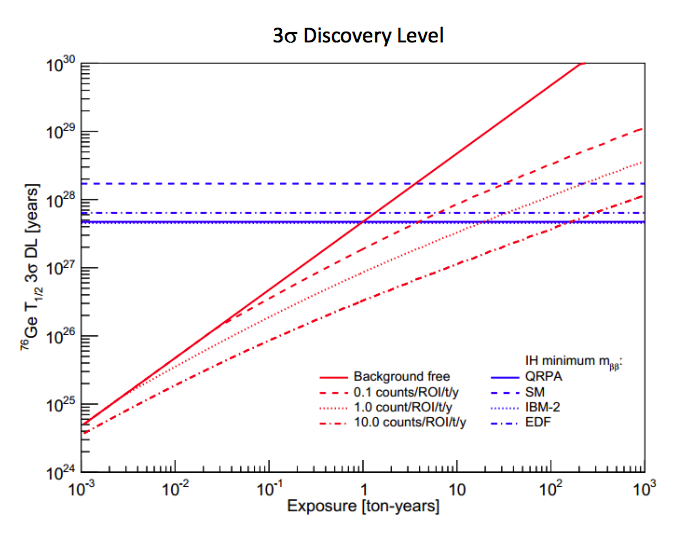
\includegraphics[width = .60\textwidth]{/Users/jgruszko/Documents/Thesis/Plots/Ch1/IH_Discovery.png} \hfil
\caption{The background requirements and exposure needed for $3\sigma$ discovery-level observation of $0\nu\beta\beta$ decay, assuming the inverted hierarchy. Plot courtesy of Jason Detwiler.}
\label{IH_Discovery}
\end{figure}

	- Gerda
\section{The \MJDemo}
\subsection{The \MJ~\MJDemo}
The \MJ~\MJDemo, the $0\nu\beta\beta$ decay search that is the focus of much of this thesis, is an experiment made up of 40 kg of PPC detectors. 30 kg of this mass is enriched to 87\% \iso{76}{Ge}, the double-beta decay parent isotope, and 10 kg is in natural-abundance detectors. The \MJDemo~uses a staged, modular approach to construction, making its techniques naturally scalable to a tonne-scale experiment. 

The largest advantage of PPCs for $0\nu\beta\beta$ decay searches is in their pulse shape characteristics. Unlike in coaxial detectors, the distance that must be traveled by a charge cloud varies depending on where in the detector it is produced, as is clear in Fig.~\ref{PPCField}. Therefore, multi-site events, in which a $\gamma$ ray deposits energy at multiple points in the crystal, have longer rise times for a given energy, and can be cut to reduce backgrounds. 

\begin{figure}[h]
\hfil 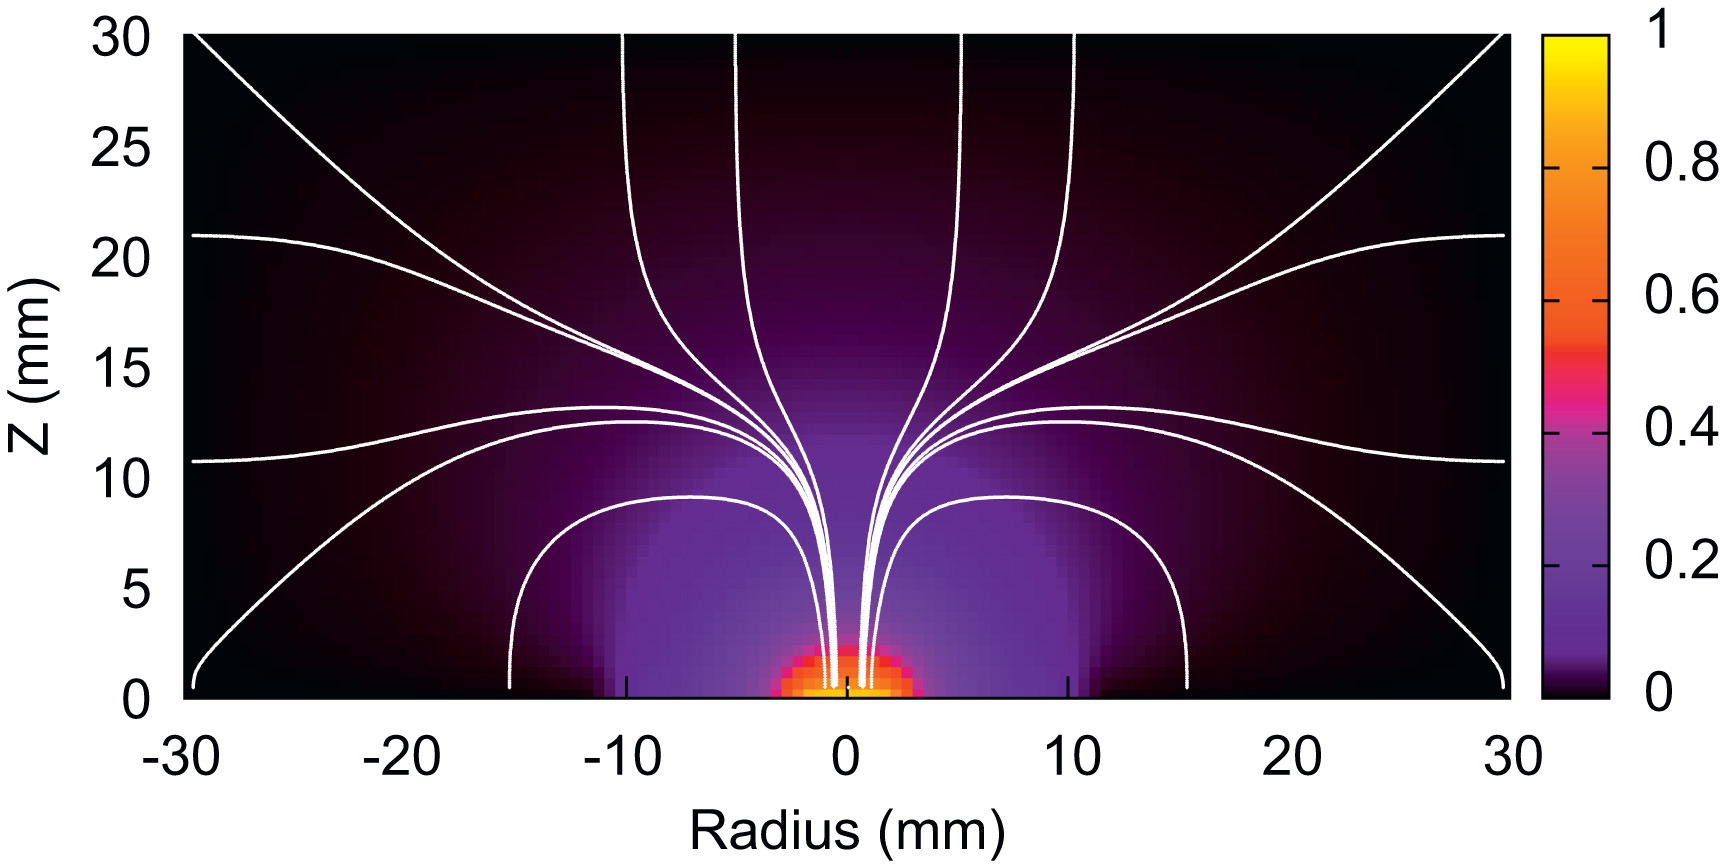
\includegraphics[width = .60\textwidth]{/Users/jgruszko/Documents/Thesis/Images/Ch1/PPCField.jpg} \hfil
\caption{A simulation of the weighting potential inside a PPC shows that charge drift paths (in white) are long and highly position-dependent. \cite{Aalseth2011}}
\label{PPCField}
\end{figure}

	- LEGeND



% ========== Chapter 2
 
\chapter {HPGe Detectors}

\section{P-Type Point Contact Germanium Detectors}
It has long been known that reducing the capacitance of High-Purity Germanium (HPGe) detectors would reduce their noise and energy thresholds. This could done by using a small ``point-like" central contact, instead of the deep well used by coaxial detectors. The first attempts to make germanium detectors with point-contact geometries were made in 1989 by Luke et. al \cite{Luke1989}. Though these detectors had much smaller capacitance than coaxial detectors, they suffered from severe charge-trapping effects, degrading the detector resolution. 

The breakthrough improvement that made this geometry useful in 2007 came with the switch from N-type to P-type detectors. i.e., in switching from drifting electrons to drifting electron holes through the crystal \cite{Barbeau2007}. Since the holes are less susceptible to trapping, PPC detectors can achieve resolutions similar to those of coaxial detectors, with electric fields created primarily through careful control of the charge impurity gradient in the bulk of the crystal. Due to their geometry, PPCs have capacitance of about 1~pF, far lower than that of similarly-sized coaxial detectors. This leads to far lower noise than is found in coaxial detectors, and therefore lower thresholds. While PPCs have masses up to 1 kg, the thresholds that can be achieved are comparable to those of small ($\sim1$~g) x-ray detectors \cite{Barbeau2007}. 


\subsection{PPCs and Low-Energy Recoils}
Because of their low thresholds and high masses, PPCs are a promising technology for low-mass WIMP searches and coherent neutrino-nuclear scattering experiments. The MALBEK and CoGeNT experiments are both low-background single-PPC experiments that have set competitive limits on (and in the case of CoGeNT, claimed observation of a signal consistent with) low-mass WIMPs \cite{MALBEK2015}\cite{COGENT2011}. One previous attempt was made to measure neutrino-nuclear scattering with a PPC \cite{BarbeauThesis}, and the COHERENT collaboration is currently considering using the technology for a future experiment at the Spallation Neutron Source \cite{CoherentSnowmassWP}. 

\subsection{Low-Energy Backgrounds in PPC Detectors}
As the tension between the MALBEK and CoGeNT results demonstrates, these measurements rely on a detailed understanding of background events near the detector threshold. Understanding these events, particularly from x-ray and $\alpha$ particle interactions, is the focus of this thesis. $\alpha$ events are also of great concern to the \MJ~ collaboration, as radon deposition on detector surfaces could contribute to backgrounds at the $0\nu\beta\beta$ Q-value. Though these backgrounds have been studied in N-type coaxial detectors \cite{JohnsonThesis2010}, this work is the first attempt to evaluate them in PPCs.

 
% ========== Chapter 5
 
\chapter{Delayed Charge Recovery Tagging}\label{ch:DCR}

%%%%%% This section should describe the signature or the methods you are trying to take advantage of %%%%%%
\section{Theory}
Alpha particles pose a problematic background in large granular detector arrays, particularly those that originate from Rn progeny that plate out on the detector surfaces during manufacturing and assembly. The \ppc\ detector technologies implemented in the \MJ\ \DEM\ have a thick (1-2 mm) outer dead layer covering most of the detector surface that is insensitive to alpha interactions originating external to or on the surface of the detector, and the point contact, despite being sensitive to these alphas, is very small in size. These features make HPGe detector arrays inherently less sensitive to alphas than, for example, bolometric arrays. 

However, between the point contact and the outer dead layer is a thin passivated surface; its response to alphas is less easy to characterize. The charge collection properties near this surface can differ for different detector models. In the \textsc{Majorana Demonstrator}, events have been observed in which alphas originating on this surface are significantly degraded in energy, leading to a potential background contribution in the region-of-interest for neutrinoless double-beta decay. 

However, it is also observed that charge mobility is drastically reduced on or near the passivated surface, and is slowly released on the timescale of waveform digitization, leading to a measurable decrease in the slope of the tail of a recorded pulse. The same effect has been observed in the TUBE alpha source scans (see unidoc).

There are two models for charge loss in the passivated surface region. One option is that this effect is due to surface propagation of the electron contribution to the signal, with the holes being collected normally. This matches the model developed in \cite{Mullowney2012}. See Fig.~\ref{fig:siggen_wf} for sample waveforms, simulated using siggen. 

\begin{figure}[h]
 \centering
 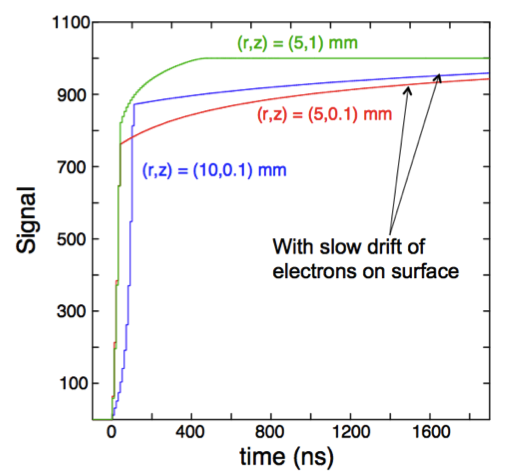
\includegraphics[height=3in]{/Users/jgruszko/Documents/Thesis/Plots/Ch3/siggen_wf}
 \caption[Simulated bulk and passivated surface waveforms]{Bulk and passivated-surface waveforms, simulated using siggen. Surface charge transport of electrons is induced by incorporating an arbitrary small amount of passivated-surface charges in the fieldgen model of the detector, which leads to electric field lines that end on the passivated surface.} 
 \label{fig:siggen_wf}
\end{figure}

In an alternative model, holes are trapped when they originate in a few-micron-thick region at the passivated surface, and then slowly re-released. Since the alpha particle's path in the detector carries it through this region and into the normal-collection bulk region, part of the energy of the event appears as a normal, fast pulse, and the remainder of the charge is collected slowly. The waveforms of the events would appear similar to those including surface electron transport. The bulk trapping and slow surface drift effects could also appear in conjunction. 

The models behave differently as the position of the alpha interaction on the passivated surface changes, so they can be distinguished using the TUBE scan results (see Sec.~\ref{sec:dcr_models}). For the purposes of this analysis, the cause of the delayed charge is irrelevant. 

Using a filter that can identify the occurrence of this delayed charge recovery, these events can be identified, allowing for the efficient rejection of passivated surface alpha events in analysis. The goal of such a filter is to detect the presence of slow charge collection occurring after the bulk charge collection has been completed. In a waveform that has been fully corrected for the electronic response function, this appears as a positive slope of the tail. In an uncorrected pulse, it appears as a tail which has a less-negative slope than is expected for that particular channel's electronics response. 

%%%%%% In this section you should validate your techniques. %%%%%% 
\section{Implementation}
For all versions of the DCR analysis cut, the relevant parameters are found using calibration data, since these runs contain a very low fraction of surface events. Version 1.0 is the version of the analysis currently in use in the \MJ\ \DEM\ analysis chain, and does not require knowledge of the electronics response function. Version 1.1 is identical to version 1.0, but with an added term that corrects for charge trapping in the bulk of the detector, reducing systematic uncertainties. It is currently under development. Version 2.0 is a proposal to be implemented in future analysis of \MJ\ \DEM\ data, which uses a full correction for the electronics response function. Optimization and error estimates are fully described for version 1.0 of the analysis, and commented on in a more limited capacity for the other versions. 

\subsection{DCR Version 1.0}
The DCR parameter is found by first calculating the slope of the waveform tail for each event in a channel. 1 $\mu$s of the waveform is averaged (corresponding to 100 waveform samples in non-multisampled data) at each of two points on the waveform. The first region lies between 2 and 3 $\mu s$ after 97\% of the waveform rise, and the second is the final $\mu s$ of the waveform (in the non-multisampled data, this is between 19 and 20 $\mu s$). See Fig.~\ref{fig:DCR_step1}. These values were chosen to avoid introducing unwanted sensitivity to the shape of the waveform turnover and to decrease sensitivity to noise. Waveforms for which no valid tail slope can be found, i.e. those in which the 97\% time point occurs too late to leave a usable tail, are flagged and automatically accepted by the DCR analysis. 

\begin{figure}[h]
 \centering
 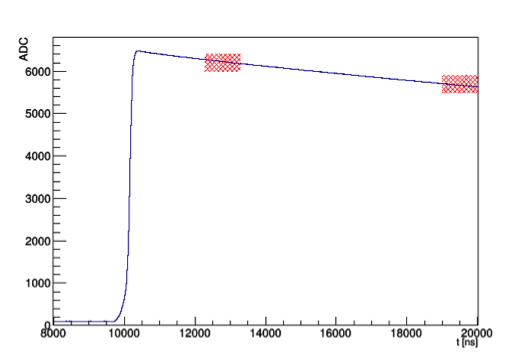
\includegraphics[height=2in]{/Users/jgruszko/Documents/Thesis/Plots/Ch3/DCR_step1}
 \caption[A sample MJD waveform, with indicated tail slope measurement points]{A sample MJD waveform. The ADC values are averaged in each of the two shaded regions. The slope between those average points is taken to be $\delta$.} 
 \label{fig:DCR_step1}
\end{figure}

\begin{figure*}[t]
 \centering
 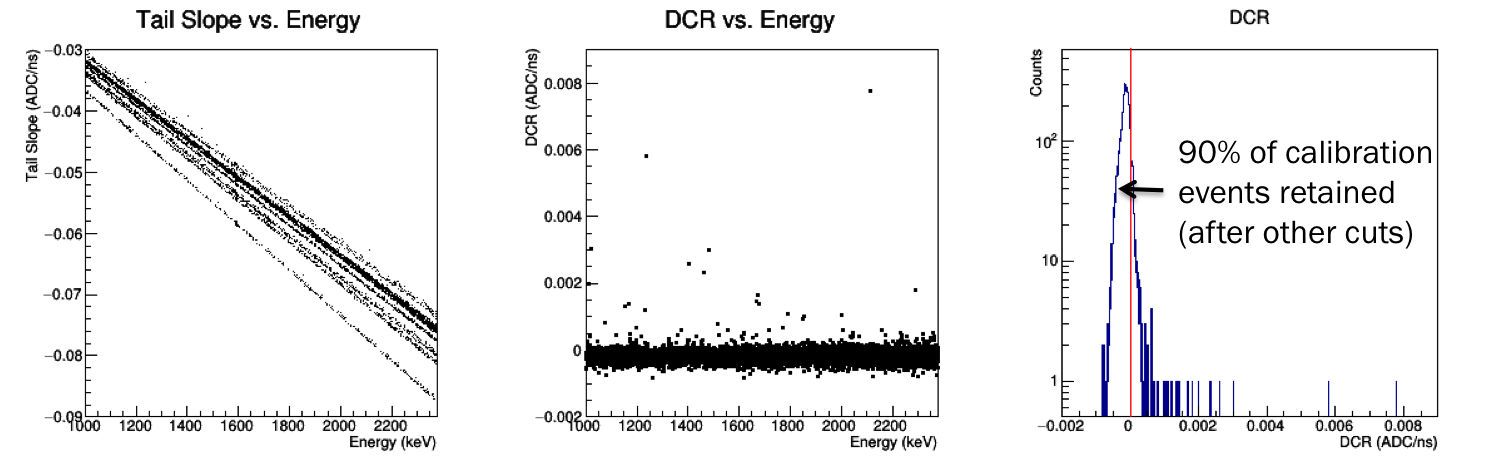
\includegraphics[width=1.0\textwidth]{/Users/jgruszko/Documents/Thesis/Plots/Ch3/DCR_implementation}
 \caption[The steps of the DCR parameter calculation]{The steps of the DCR parameter calculation, plotted for all high gain channels in DS3 detectors. {\it Left:} $\delta$ vs. Energy is plotted and fit with a line for each channel. {\it Center:} The fit parameters are used to calculate the raw DCR value, which is then shifted such that 90\% of single-site calibration events in this energy range fall below 0. {\it Right:} The DCR distribution displays a gaussian distribution with a high-DCR tail.} 
 \label{fig:DCR_implementation}
\end{figure*}

Assuming that the tail of bulk-event waveforms has an exponential form, the slope $\delta$ is:
$$\delta = \frac{y_1 - y_2}{t_1-t_2} = A\frac{e^{\frac{-t_1}{\tau}}-e^{\frac{-t_2}{\tau}}}{t_1-t_2} $$
where $y_1$, $y_2$, $t_1$ and $t_2$ correspond to the average values and times for each of the two regions, $A$ is the waveform amplitude, and $\tau$ is the decay constant of the tail. 

To first order in $t_n/\tau$, 
$$\delta = \frac{A}{\tau}$$
for bulk events. 

The tail slope is plotted with respect to energy for each channel. Using single-site events with energies between 1\,MeV and 2.38\,MeV (the Compton shoulder of the $^{208}$Th 2614 keV peak), a line is fit to the resulting distribution, and the parameters of that fit are used to project $\delta$ on to the energy axis. This is equivalent to finding the average decay constant for the pulses in a channel and doing a first-order pole-zero correction of the waveforms prior to measuring their tail slope. 

The resulting value is defined as the raw DCR parameter for the waveform:
$$\mathit{DCR_{raw}} = \Delta - (\frac{a}{\tau}E+b)$$
where $a$ is a scaling constant that converts between pulse amplitude and energy for the channel. $b$, which is generally positive, is a constant determined by the fit that corrects for the fact that a waveform with signal height 0 will have a positive estimated energy when the maximum value of a trapezoidal filter is used as the energy estimate. 

The calibration run events have a median raw DCR of 0, with low tail slope events (i.e. events occurring near the passivated surface) having larger DCR values. The width of the gaussian part of the DCR distribution in the calibration data is primarily determined by the noise and energy nonlinearity of the channel. The high-DCR tail is due to passivated-surface events, transition-layer multisite events (see Fig.~\ref{fig:DCR_PS}) and other multi-site events that go untagged by A/E and pile-up cuts, and an additional contribution that depends on the bulk charge trapping of the detector (see Sec.~\ref{ssec:dcr_ct} for details). 

The cut value $c$ is set to reject 1\% of the single-site events with energies between 1\,MeV and 2.38\,MeV in the calibration data set used to determine the cut parameters. Single-site events are selected using  A vs. E analysis and additional pile-up cleaning cuts (see Data Cleaning unidoc section).
To set the ``corrected DCR" (DCR\textsubscript{corr}) value (hereafter referred to simply as ``DCR"), the raw DCR value is shifted such that the rejected events have DCR\textsubscript{corr}$>0$:
$$\mathrm{DCR}\textsubscript{corr} = \Delta - (\frac{a}{\tau}E+b) - c$$
This value is then calculated for all background events. 


\subsection{Energy Non-Linearity Effect}
The non-linearity of the waveform digitization has a significant effect on the efficiency of the cut at a given energy. Though much of the variation in efficiency is removed by nonlinearity correcting each waveform \cite{EnergyUnidoc}, a systematic variation with energy remains, as seen in the variation of the Compton continuum acceptance in  Figure \ref{fig:dcr99_eff}. This effect differs from channel to channel, with low-gain channels displaying higher variation. The variation due to this effect is highly dependent on the chosen bulk acceptance efficiency; at high acceptance levels, the effect is greatly reduced. 

\begin{figure}[t]
 \centering
 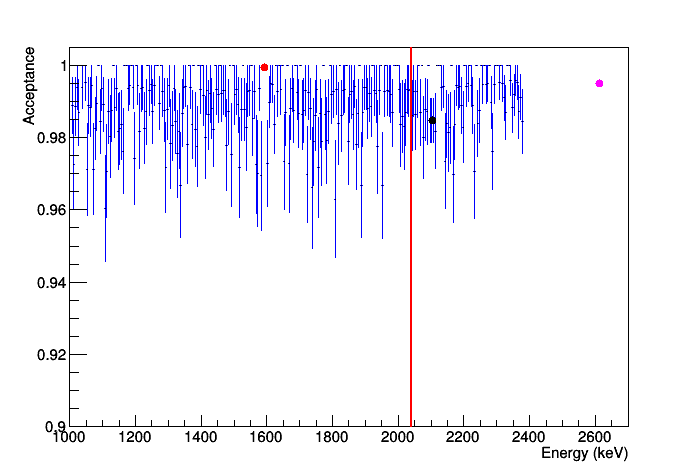
\includegraphics[height = 3in]{/Users/jgruszko/Documents/Thesis/Plots/Ch3/Ch640_dcr99_eff.png}
 \caption[99\% acceptance DCR cut efficiency and uncertainties]{Efficiency plot for the 99\% acceptance DCR cut in P42665A, a typical detector in DS3. The acceptance in the $^{208}$Th DEP, SEP, and FEP are indicated by the red, black, and magenta points, respectively. The blue points indicate the acceptance in each 5\,keV bin of the Compton continuum. The red line indicates the 3\,keV \nonubb\ ROI.} 
 \label{fig:dcr99_eff}
\end{figure}

This cannot be correctly termed an uncertainty of the cut, since the energy of a given event is well-known, as is the DCR efficiency at a given energy. A gain uncertainty of 0.4\,keV, larger than that observed in any data set \cite{EnergyUnidoc} leads to a DCR efficiency change of less than 0.2\%, which is negligible compared to the other DCR uncertainties, so this uncertainty is neglected. 

The non-linearity effect will change the spectral shape of the remaining events, however. When estimating an integral rate over some region, the DCR acceptance should be calculated for that particular region, so that bias is not introduced. For the \nonubb\ limit calculation, the DCR efficiency is calculated in a 3\,$\sigma$-window around the \nonubb\ Q-value. 

\subsection{Optimization}
As described in \cite{Detwiler_sensitivity}, the sensitivity to the \nonubb\ decay half-life, in the presence of backgrounds, is proportional to $\frac{\epsilon}{\sqrt{N_b}}$, where $\epsilon$ is the cut acceptance and $N_b$ is the number of background events. In this case, the energy range used to find the number of background events is the disjoint 350\,keV window around the \nonubb\ Q-value that is used to estimate the background level in the ROI. The event energies included those from 1950 to 2350\,keV, with the exception of the regions from 2094 to 2127\,keV and 2195 to 2212\,keV, where the \MJ\ background model predicts the presence of gamma background peaks. 

An optimization study was conducted using the open data from \MJ\ \DEM\ data sets 0 to 4. See Table.~\ref{tab:DS_summary} for descriptions and exposures of each data set. Data set 5 was excluded from this study due to the known elevated noise rate in its first half, which distorts the DCR distribution and reduces the effectiveness of the analysis. Only enriched detectors were included in the optimization study, since these detectors dominate the \DEM 's sensitivity to \nonubb . 

For this study, the sensitivity was evaluated at a range of DCR calibration-event acceptance levels, varying from 90\% to 100\%. See Table~\ref{tab:DCR_opt}. Based on the results, the DCR acceptance level was chosen to be 99\%. 

Higher acceptance levels are being considered for multi-sampled data, since the longer duration of the waveform tail leads to a more-sharply peaked DCR distribution for bulk events. See Figure~\ref{fig:DS2_DS3_comparison}. Though the open exposure in this data set is low, and higher statistics are needed to make a definitive recommendation, studies of DS 2 suggest that a 99.9\% acceptance DCR cut may be the optimal choice for multi-sampled data. Acceptances over 99\% were also studied in DS 0-1 and 3-4 and were found to be suboptimal. 

\begin{table}[]
\centering
\begin{tabular}{l l | l l l l}
DS &  $\epsilon$ (\%) & $N_{b}$ (counts) & $\frac{N_{b}}{\epsilon}$ (arb.) & $N_{b, enr}$ (counts) &$\frac{N_{b, enr}}{\epsilon}$ (arb.) \\    
\hline
0 &                  100 &        79 &             1.13e-01$\pm$5.63e-02 &                   69 &             1.20e-01$\pm$6.02e-02 \\
 &                   99 &        14 &             2.65e-01$\pm$1.32e-01 &                   10 &             3.13e-01$\pm$1.57e-01 \\
 &                   95 &        14 &             2.54e-01$\pm$1.27e-01 &                   10 &             3.00e-01$\pm$1.50e-01 \\
 &                   90 &        14 &             2.41e-01$\pm$1.20e-01 &                   10 &             2.85e-01$\pm$1.42e-01 \\
\hline
1 &                  100 &      49 &             1.43e-01$\pm$7.14e-02 &                   46 &             1.47e-01$\pm$7.37e-02 \\
 &                   99 &       6 &             4.04e-02$\pm$2.02e-02 &                    3 &             5.72e-02$\pm$2.86e-02 \\
 &                   95 &       6 &             3.88e-02$\pm$1.94e-02 &                    3 &             5.48e-02$\pm$2.74e-02 \\
 &                   90 &       6 &             3.67e-02$\pm$1.84e-02 &                    3 &             5.20e-02$\pm$2.60e-02 \\
\hline               
2 &                  100 &      7 &             3.78e-01$\pm$1.89e-01 &                    6 &             4.08e-01$\pm$2.04e-01 \\
 &                   99.9 &       0 &                  inf$\pm$inf &                    0 &                  inf$\pm$inf \\
 &                   99.5 &       0 &                  inf$\pm$inf &                    0 &                  inf$\pm$inf \\
 &                   99 &       0 &                  inf$\pm$inf &                    0 &                  inf$\pm$inf \\
 &                   95 &       0 &                  inf$\pm$inf &                    0 &                  inf$\pm$inf \\
 &                   90 &       0 &                  inf$\pm$inf &                    0 &                  inf$\pm$inf \\
\hline              
3 &                  100 &     25 &             2.00e-01$\pm$1.00e-01 &                   21 &            2.18e-01$\pm$1.09e-01 \\
 &                   99 &      2 &             7.00e-01$\pm$3.50e-01 &                    0 &                  inf$\pm$inf \\
 &                   95 &      2 &             6.72e-01$\pm$3.36e-01 &                    0 &                  inf$\pm$inf \\
 &                   90 &      2 &             6.36e-01$\pm$3.18e-01 &                    0 &                  inf$\pm$inf \\
\hline
4 &                  100 &     17 &             2.43e-01$\pm$1.21e-01 &                   16 &             2.50e-01$\pm$1.25e-01 \\
 &                   99 &      1 &             9.90e-01$\pm$4.95e-01 &                    0 &                  inf$\pm$inf \\
 &                   95 &      1 &             9.50e-01$\pm$4.75e-01 &                    0 &                  inf$\pm$inf \\
 &                   90 &      1 &             9.00e-01$\pm$4.50e-01 &                    0 &                  inf$\pm$inf \\
\end{tabular}
 \caption[DCR optimization studies for the \DEM ]{DCR optimization studies in DS 0 to 4 show that the sensitivity of the cut is optimized at 99\%. Results in DS2 suggest that higher acceptances, up to 99.9\%, may be optimal when multi-sampling is used.} 
 \label{tab:DCR_opt}
\end{table}


\begin{figure}[h]
 \centering
 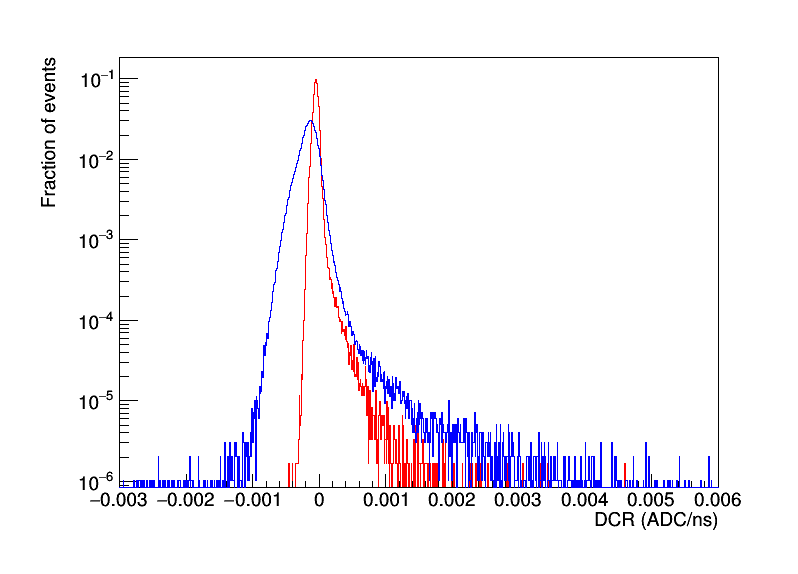
\includegraphics[height=3in]{/Users/jgruszko/Documents/Thesis/Plots/Ch3/DS2_DS3_cont_forUnidoc.png}
 \caption[Comparison of DCR in singly-sampled and multi-sampled MJD data sets]{DCR of single-site Compton continuum events in calibration data, in multisampled data (DS2, in red) and singly-sampled data (DS3, in blue). In DS 2, DCR is more sharply peaked for bulk events, allowing for a higher-acceptance DCR cut that retains the same sensitivity to alpha events.} 
 \label{fig:DS2_DS3_comparison}
\end{figure}


\subsection{Uncertainty Estimation}
\subsubsection{Stability}
To study DCR stability over time, calibration skim files are chained together and analyzed.  DCR values for every event are plotted as a function of time, with time presented as the number of minutes elapsed since the beginning of the first calibration, with non-calibration periods removed from the timeline. See Fig.~\ref{fig:DS3_stab}, {\it top}. Only calibrations from the Module 1 source are used in the DS0-DS3 analysis, and only calibrations from the Module 2 source are used in the DS4 analysis.  Calibrations from both sources are used in the DS5 analysis. Calibration runs with timing or quality issues are removed from all analyses.  

Only single-site (as determined by {\tt avse} and {\tt nX} cuts) events in ``{\tt isGood}" detectors that pass data-cleaning cuts are included in the analysis. The energy window used for the \nonubb\ analysis is 2028\,keV - 2050\,keV. A second analysis of the $^{208}$Tl DEP (1590\,keV - 1595\,keV) is also conducted. A 40-minute moving average of the DCR values within the closed range [-0.003,0.035] is calculated. The larger upper bound was chosen to catch events with a high DCR due to mis-calibrations in the energy parameter {\tt trapENMCal}. The mean DCR value is then plotted at the central time value within each forty-minute window (see Fig.~\ref{fig:DS3_stab}, {\it middle}). Data points from the first and last forty minutes are excluded to eliminate bias due to window effects. 

The DCR cut efficiency (i.e.  the percentage of events within the window with {\tt dcr90<0}) over time is plotted using the same moving-average algorithm, as in Fig.~\ref{fig:DS3_stab}, {\it bottom}. Note that this method of calculating efficiency differs from the standard efficiency calculation, which weights each detector's efficiency by its active mass.  An effort to employ this method in the stability analysis is currently under development. A one-dimensional histogram is created out of the efficiency values over time, and the standard deviation of this distribution is taken to be the uncertainty in the efficiency of DCR over time, $\sigma_{stab}$. 

This analysis is conducted for high- and low-gain channels in each data set. Results are given in Table~\ref{tab:DS_efficiencies}. If the efficiency deviates by more than $2\sigma_{stab}$ in a set of calibration runs, the DCR parameters are re-evaluated using the relevant runs and a stability correction is applied. Stability corrections to DCR are also applied when a stability correction is needed in the A vs. E analysis \cite{AvsE_unidoc}.

The current version of the analysis employs one to two longer (8 to 12 hour) energy calibrations to set the cut in each data set. 

\begin{sidewaysfigure}[]
 \centering
 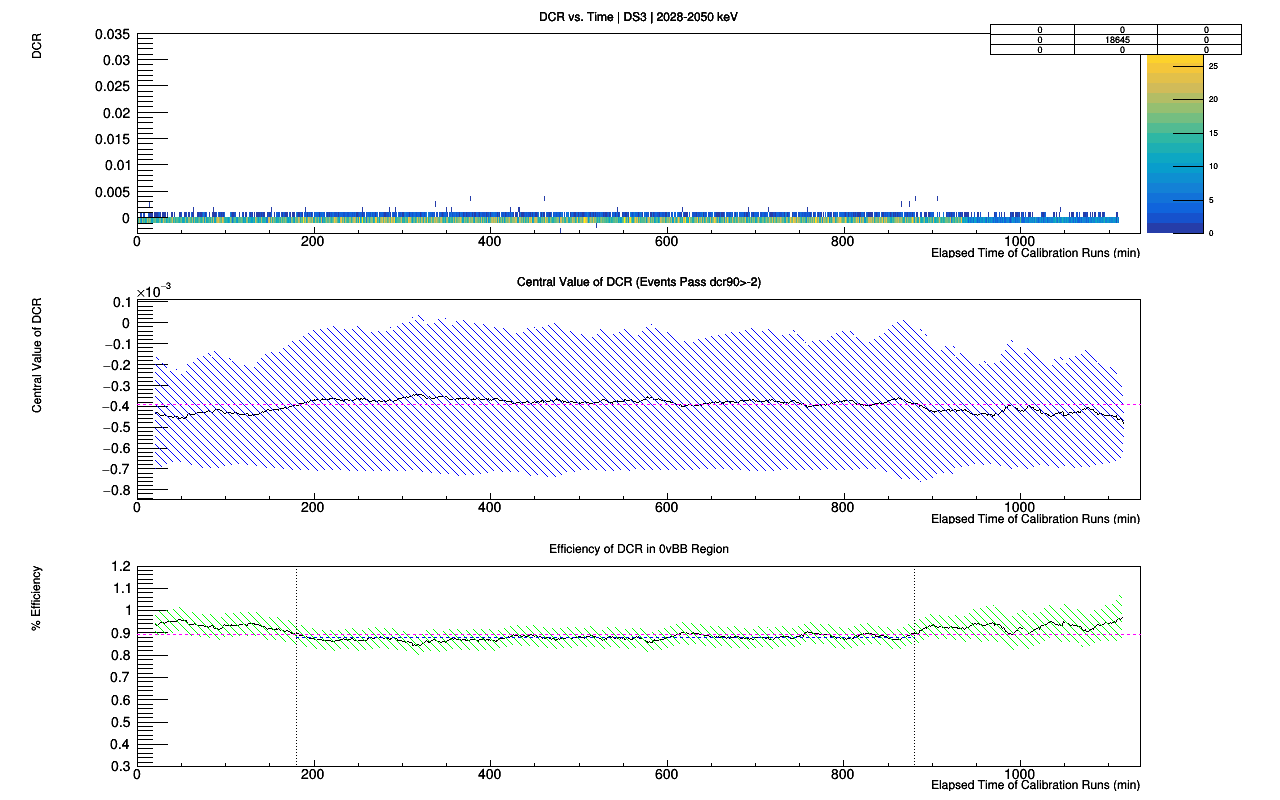
\includegraphics[width=1.0\textwidth]{/Users/jgruszko/Documents/Thesis/Plots/Ch3/DS3_stab}
 \caption[DCR stability study results in DS3 high-gain channels]{Stability study results for DS3 high-gain channels. The middle and bottom figures are calculated using a 40-minute moving average; in these plots the filled dashed region indicates the uncertainty in each value, taken as the standard deviation of the value's distribution in a given time window. The magenta lines indicate the mean of the plotted values. {\it Top:} DCR values for all events passing cuts. {\it Middle:} The central value of DCR over time. {\it Bottom:} The bulk acceptance of the DCR cut over time. The vertical lines indicate the runtime boundaries of the long calibration run used to set the DCR cut, and the blue line indicates the average efficiency in this time window. Plots courtesy of Chris Haufe.} 
 \label{fig:DS3_stab}
\end{sidewaysfigure}


\subsubsection{Statistical Uncertainty}
In each channel, the statistical uncertainty of the cut efficiency is $\frac{\sigma}{N} = \frac{1}{\sqrt{N}}$, where $N$ is the number of events rejected by the DCR cut in the set of calibration runs used to set the cut, in the energy window being used. See Table~\ref{tab:DS_efficiencies} for the uncertainties in the \nonubb\ efficiency window.

\subsubsection{Pulse-Shape Bias}
Irregularities in the pulse shapes of events, particularly charge-trapping re-release and multi-site effects, can have an effect on the calculated DCR acceptance. Events with a transition layer multi-site component, multi-site events occurring very near the point contact, and events with high charge trapping, like those seen in \ref{fig:DCR_PS}, may be untagged by A vs. E and data cleaning analyses, but will be accepted by the DCR cut with lower-than-average efficiency. A visual examination of the calibration events rejected based on their DCR values shows many of them to be of this type.

To quantify the uncertainty introduced by these effects, we compare the DCR acceptance in a 3$\sigma$ window centered on the $^{228}$Th double-escape peak (DEP), a known sample of single-site events, to the average acceptance in the left- and right-hand sidebands of the peak. The difference is cited as the pulse shape-dependent bias ($\sigma_{PS}$) for each channel. This value is generally positive, indicating that the acceptance in the DEP is higher than the average acceptance, and therefore that we have taken a conservative estimate of the DCR efficiency. The overall bias is given by an exposure-weighted average of the bias in each channel, since $\sigma_{PS}$ is assumed (conservatively) to be fully correlated among the detectors. 

The pulse shape bias indicates that the DCR analysis is effectively tagging some fraction of the multisite gamma events that go untagged by the A vs. E analysis. This implies that the DCR analysis has power for rejecting background gamma events in addition to alpha events.

\begin{figure}[]
 \centering
 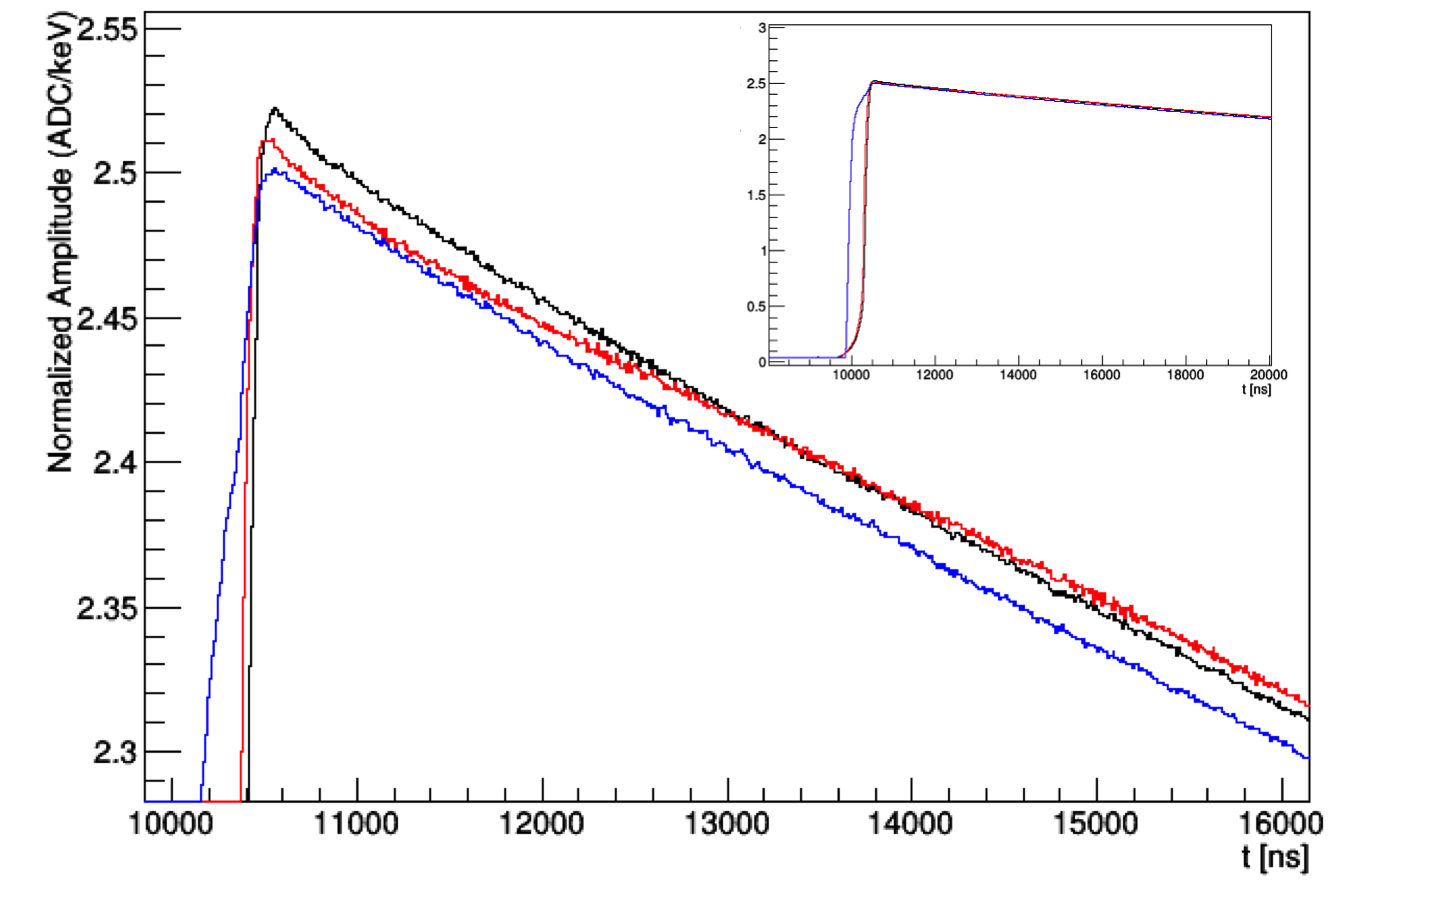
\includegraphics[width=1.0\columnwidth]{/Users/jgruszko/Documents/Thesis/Plots/Ch3/DCR_PS}
 \caption[Sample waveforms demonstrating the effect of pulse-shape on DCR]{The effect of pulse-shape on DCR, in one channel. The event drawn in black passes the DCR cut, those in blue and red fail the cut. The event in blue is thought to be a near-point-contact multi-site event, where the late charge arrival from the second site gives it an ``incorrect" energy for its tail slope. The one in red is thought to be a transition-layer multisite event or an event with high bulk charge trapping, either of which would contribute the additional slow component that changes its tail slope. All events are normalized by their max-pickoff energy ({\tt trapENMCal}), which is the energy estimator used in the DCR calculation.} 
 \label{fig:DCR_PS}
\end{figure}

\subsection{DCR Version 1.1}\label{ssec:dcr_ct}
Version 1.1 of the DCR analysis is currently being tested. This version corrects for the effect of bulk charge trapping in the detectors on the tail slope. It is being developed in an attempt to reduce the pulse-shape systematic uncertainty of the cut acceptance. Correcting for this effect will also reduce the overall width of the DCR distribution, allowing for a more effective cut at the same level of bulk-event sacrifice, and correct the slight broadening of the DCR distribution with increasing energy. 
 
\subsubsection{Bulk Charge Trapping and the DCR Distribution}
The bulk charge trapping in a given detector can be measured by its energy resolution improvement when the effective pole-zero charge trapping correction is applied. Using this method we can comparing the DCR vs. energy distributions for high charge-trapping detectors and low charge-trapping detectors, as in Fig.~\ref{fig:ct_DCRvE}. It is clear that for detectors with minimal charge trapping, the DCR distribution is narrower and that all portions of a peak, like the $^{208}$Tl double escape peak (DEP) shown, have consistent DCR acceptance. For a detector with high charge-trapping, on the other hand, the low-energy tail, which contains the events in which charge-trapping has occurred, has higher DCR values than the bulk of the peak. This matches the effect that would be expected if bulk trapped charge were being released on a 2-3 $\mu$s timescale, adding a slow additional component to the tail slope and making it less negative. 

This effect contributes to $\sigma_{PS}$ because the gaussian portion of the DEP is made up of events that are particularly unlikely to have been affected by bulk charge trapping (since if they were affected by trapping, they would occur in the low-energy tail of the peak). In detectors that have high bulk charge-trapping, this peak will therefore have higher DCR acceptance than the Compton continuum, which is made up of events with a normal incidence of charge trapping, making $\sigma_{PS}$ large for that detector. 

\begin{figure}[]
 \centering
 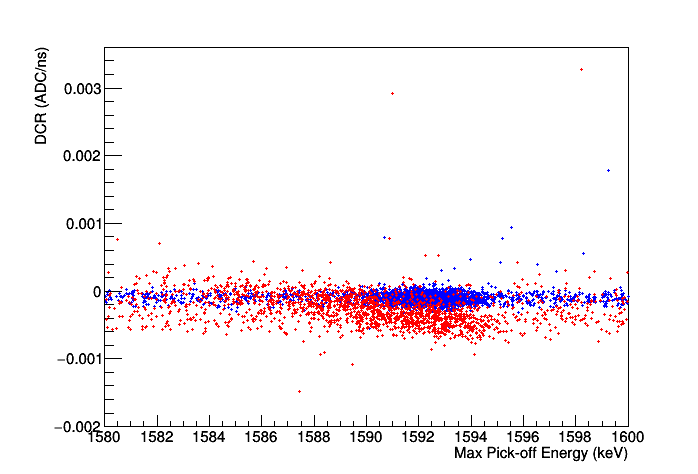
\includegraphics[width=1.0\columnwidth]{/Users/jgruszko/Documents/Thesis/Plots/Ch3/ChargeTrappingStudy_trapENMCal.png}
 \caption[The effect of bulk charge trapping on DCR in the $^{208}$Tl DEP and surrounding continuum.]{The effect of bulk charge trapping on DCR in the $^{208}$Tl DEP and surrounding continuum. The points in red are from detector P42537A, which exhibits a 3 keV FWHM improvement in the 2614 keV peak when charge-trapping is corrected. The points in blue are from detector P42661A, which exhibits a 0.4 keV improvement. The energy shown here, which is used to calculate the DCR value, is {\tt trapENMCal}. This max pick-off energy does not employ the charge-trapping correction.} 
 \label{fig:ct_DCRvE}
\end{figure}

The presence of bulk charge trapping also broadens the overall DCR distribution, increasing the tail of the distribution with high values of DCR. The amount of trapped charge in an event at a given position in the crystal is expected to be a constant fraction of the total energy, so the broadening due to this effect will increase with energy. This causes the fall in DCR cut efficiency with increasing energy observed at higher-sacrifice cuts, as seen in the left-hand plot of Fig.~\ref{fig:singleCh_eff}. 

\begin{figure*}[t]
 \centering
 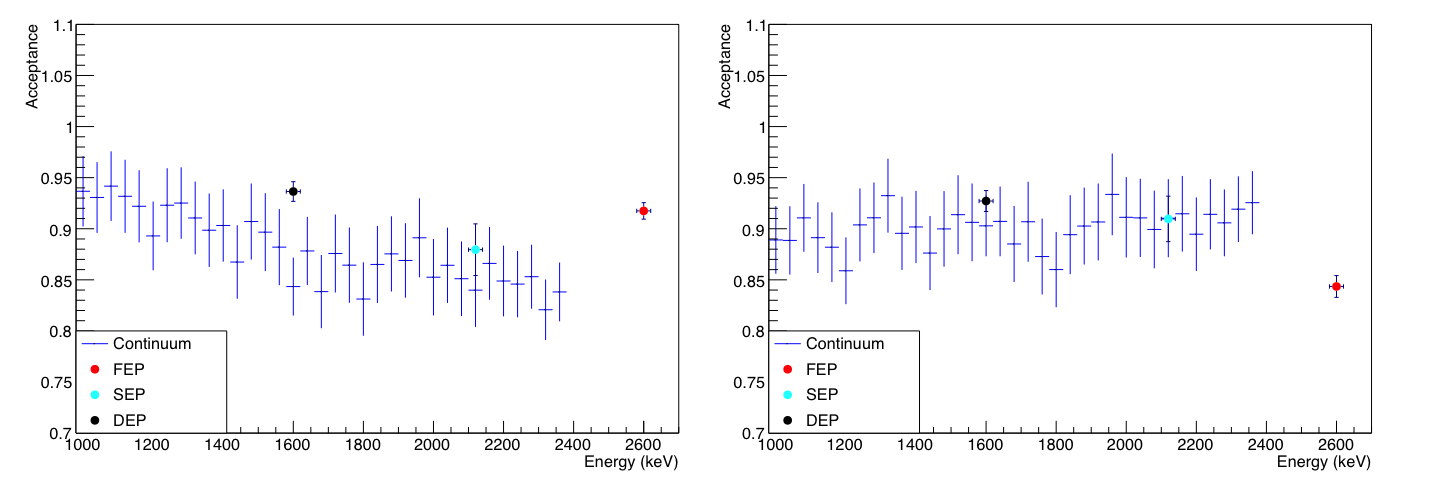
\includegraphics[width=1.0\textwidth]{/Users/jgruszko/Documents/Thesis/Plots/Ch3/sample_eff_dcr90}
 \caption[DCR cut efficiency and uncertainties]{Efficiency plots for the 90\% acceptance DCR cut in P42537A, DS3. {\it Left:} DCR cut efficiency. The pulse-shape systematic uncertainty for the channel can be calculated from the values indicated on this plot, and the energy-scale effect is clearly visible. {\it Right:} The charge-trapping-corrected DCR efficiency. The correction has reduced $\sigma_{PS}$ and the overall energy dependence has been corrected, but the efficiency is lower than expected in the full-energy 2614 keV peak. This requires further study.} 
 \label{fig:singleCh_eff}
\end{figure*}

\subsubsection{Correcting DCR for Charge Trapping}
The charge trapping effect on DCR can be corrected because the distinctive trapping and re-release timescales can be calculated from calibration data. Therefore, for a known level of charge trapping in an event, its re-release effect on the waveform tail can be subtracted from $\delta$, and then the DCR parameter can be calculated in the usual fashion from the remaining tail slope. 

The amount of charge trapping in a given event can be quantified; it is given by the difference between the charge trapping-uncorrected and corrected energies, $\Delta E$:
$$\Delta E =  {\tt trapENFCal}-{\tt trapENMCal} $$
The dependence of $\delta$ on the trapping is found by plotting $\delta$ vs. $\Delta_{E}$ and fitting with a line of slope $\ell_{E}$, as Fig.~\ref{fig:DeltaE}. The energy dependence of this slope is then fit with an exponential function, shown in Fig.~\ref{fig:DeltaEfit}. Then, for a given event, the charge trapping-corrected tail slope $\delta_{CTC}$ is:
$$\delta_{CTC} = \delta - (Ae^{\lambda E})\Delta E$$
where $A$ and $\lambda$ are the parameters found in the exponential fit.The DCR parameters are then calculated as in Version 1.0, leading to a narrower DCR distribution, with less of a high-DCR tail, as in Fig.~\ref{fig:ct_corr_DCR}.

Preliminary tests show that the use of the charge trapping correction improves $\sigma_{PS}$ and the energy-dependence of the DCR cut in detectors with significant charge trapping, but further study is needed to understand its effect in the full-energy peak. See Fig.~\ref{fig:singleCh_eff}. 

\begin{figure}[]
 \begin{subfigure}[t]{.45\textwidth}
 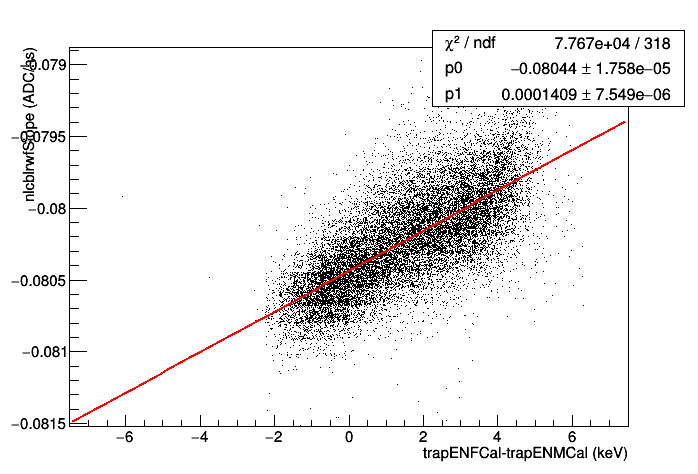
\includegraphics[width=1.0\columnwidth]{/Users/jgruszko/Documents/Thesis/Plots/Ch3/DeltaE}
 \caption{$\delta$ vs. $\Delta$E is plotted and fit with a line of slope $\ell_E$, in red, for each energy peak.}
 \label{fig:DeltaE}
 \end{subfigure}
~
 \begin{subfigure}[t]{.45\textwidth}
 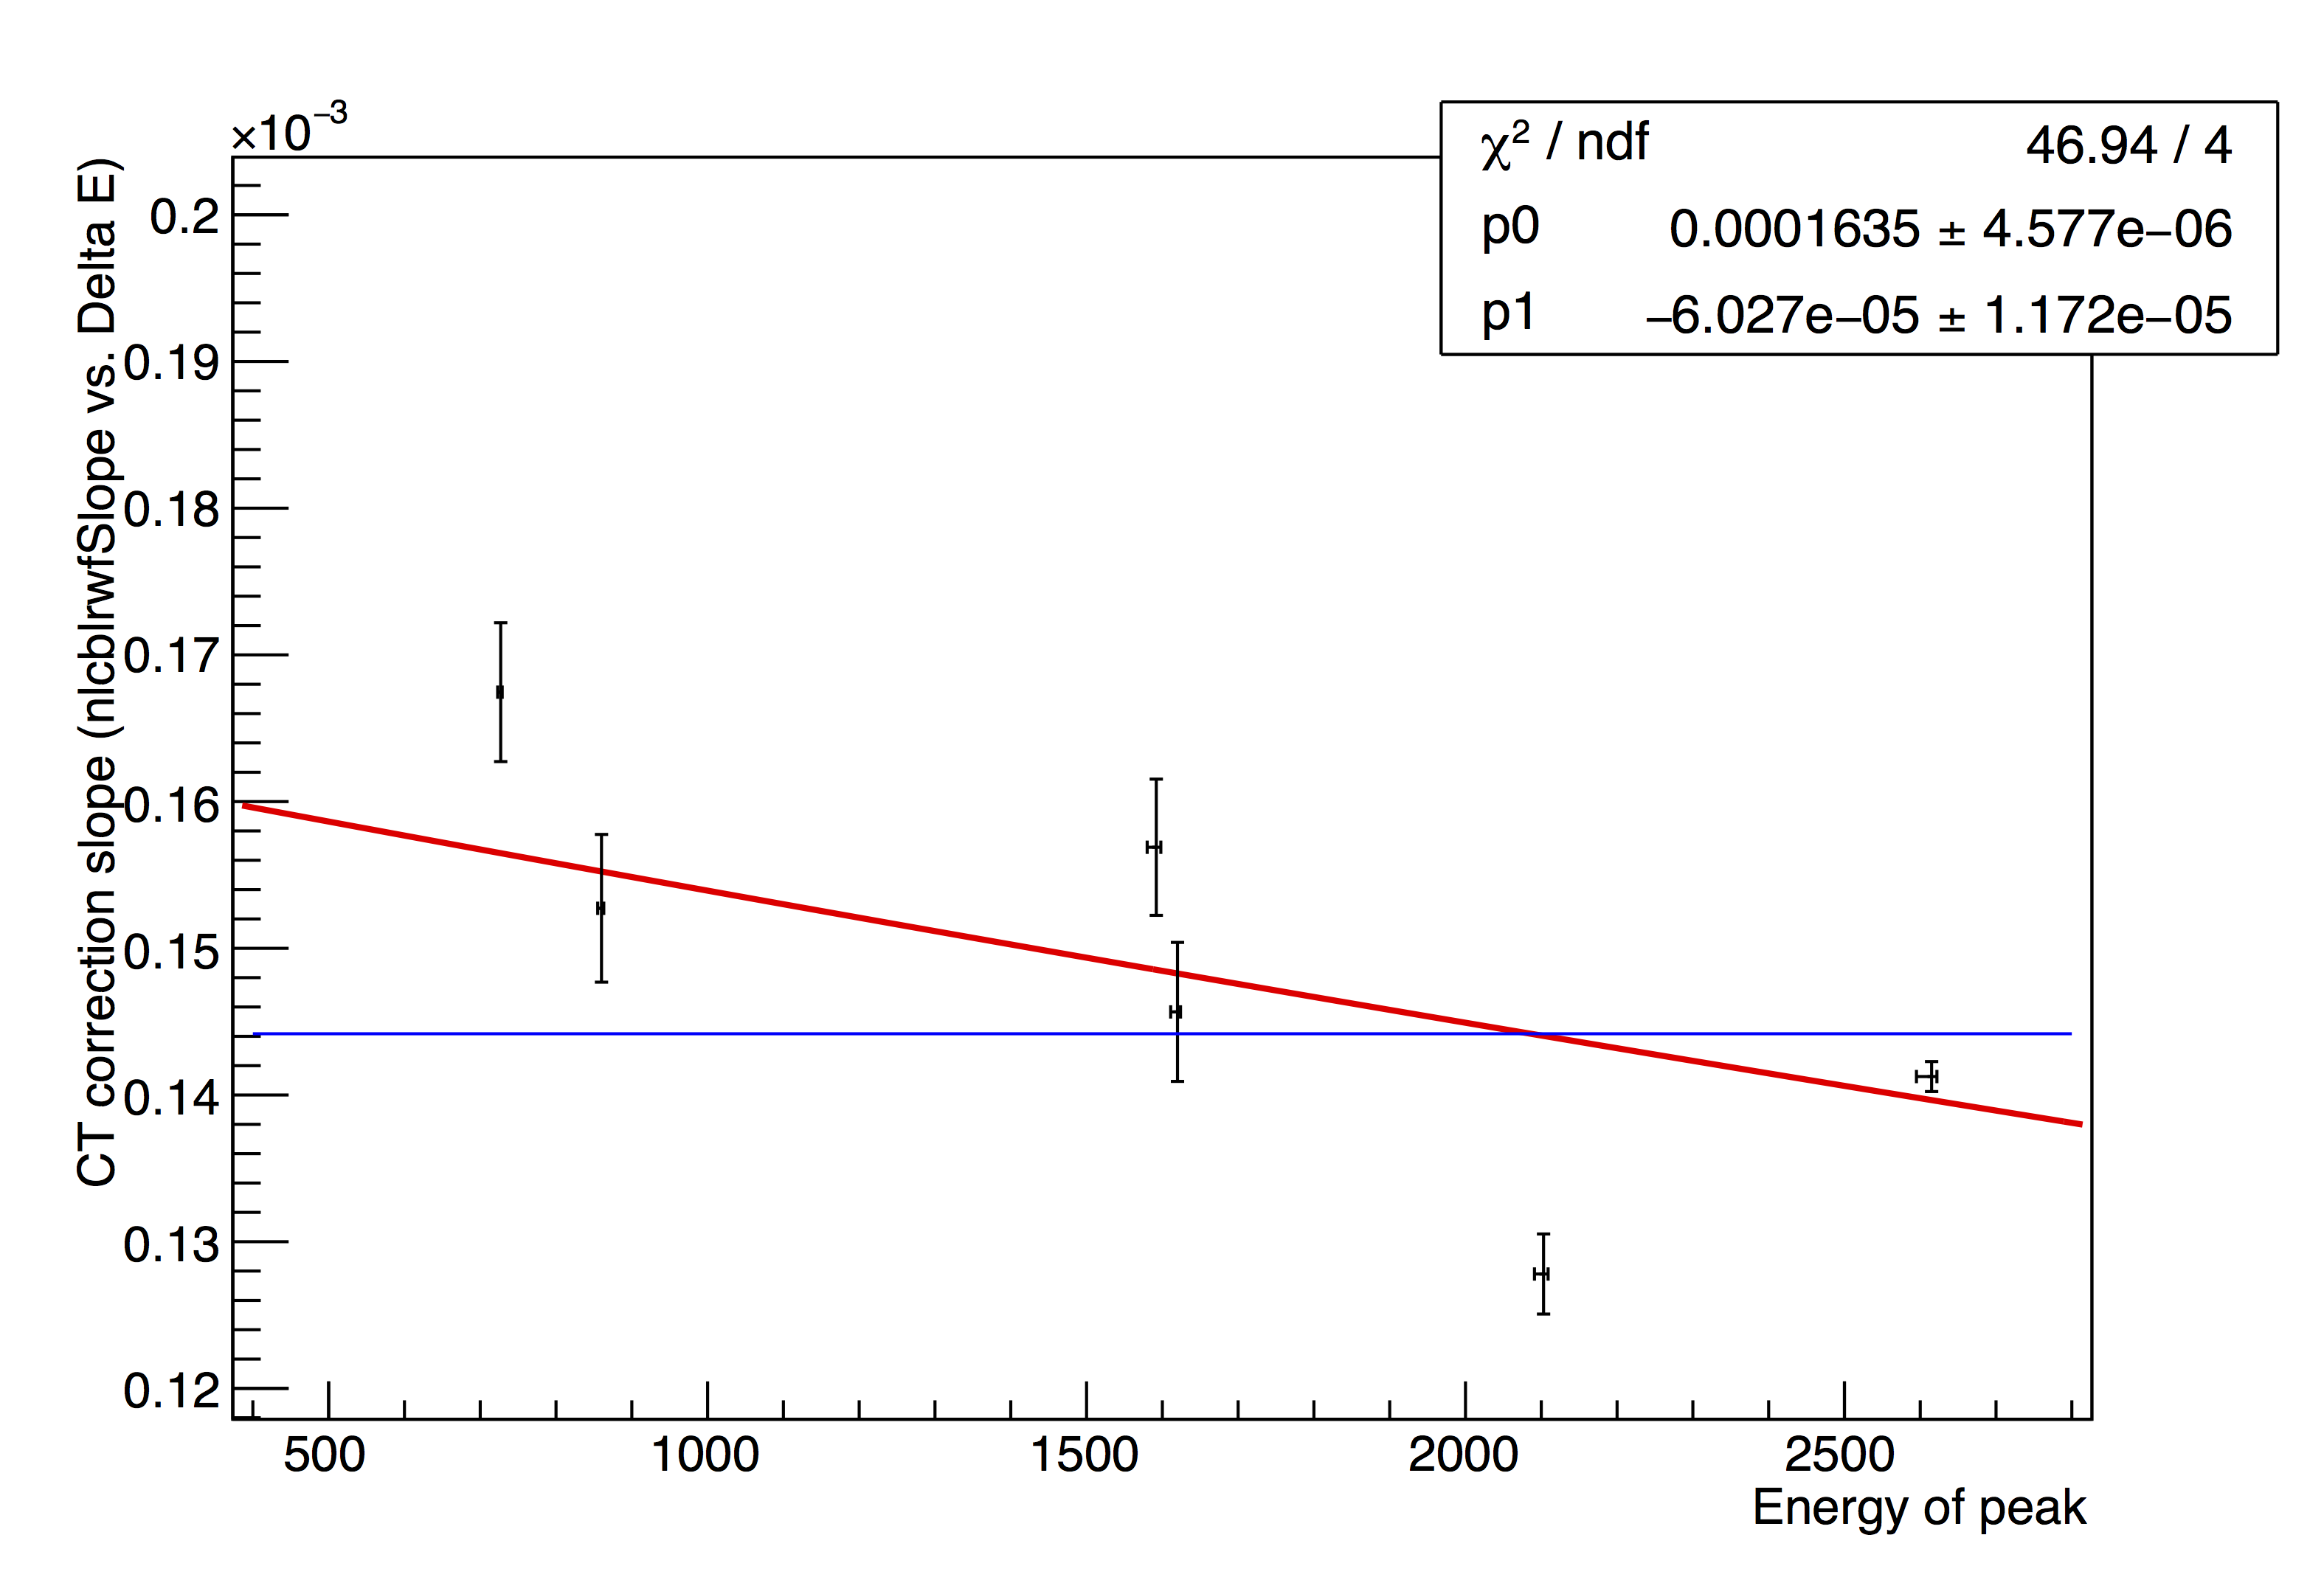
\includegraphics[width=1.0\columnwidth]{/Users/jgruszko/Documents/Thesis/Plots/Ch3/DeltaEfit.png}
 \caption{$\ell_E$ is plotted with respect to E and fit with an exponential, in red. The assumption of constant $\ell_E$, in blue, is a poor model of the observed behavior.}
 \label{fig:DeltaEfit}
 \end{subfigure}
   \centering
 \begin{subfigure}[]{.7\textwidth}
 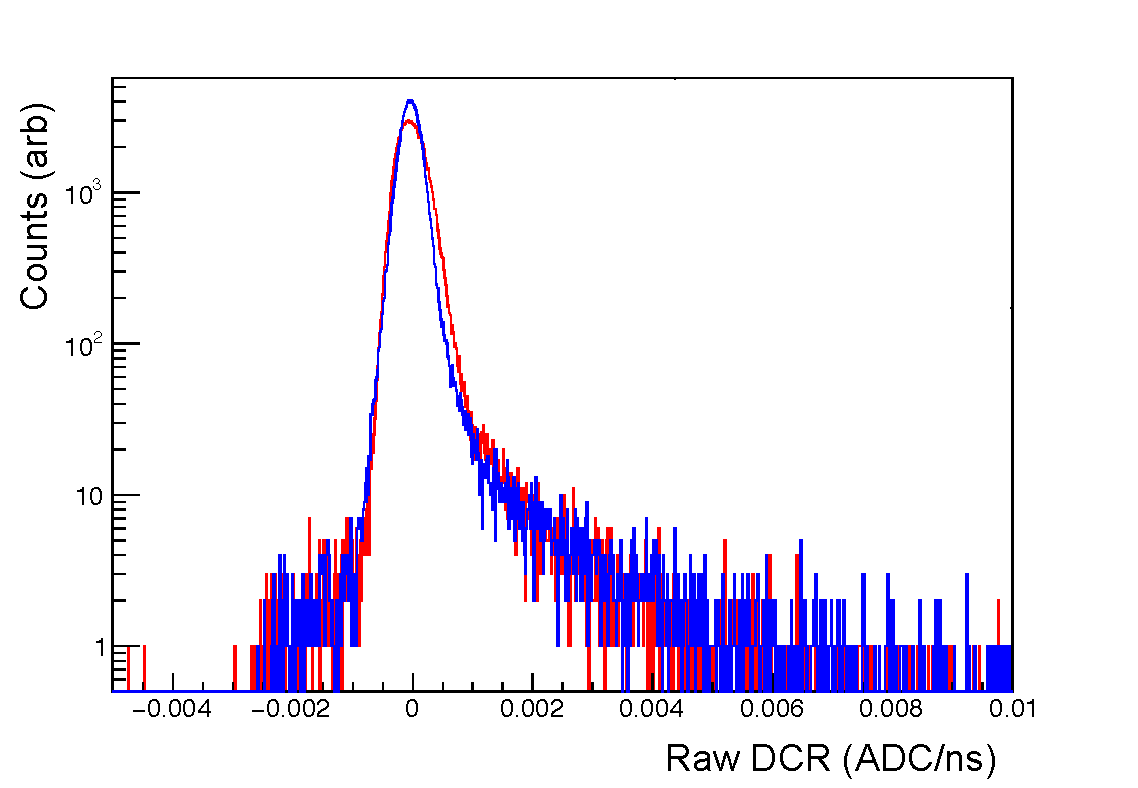
\includegraphics[width=1.0\columnwidth]{/Users/jgruszko/Documents/Thesis/Plots/Ch3/ct_corr_DCR}
 \caption{When corrected using the resulting parameters, the charge-trapping-corrected DCR distribution in the 1 to 2.38\,MeV range, in blue, is narrower and with a smaller high-DCR tail than the uncorrected distribution, in red.}
 \label{fig:ct_corr_DCR}
 \end{subfigure}
 \caption[The steps of the charge trapping tail slope correction]{The steps of the charge trapping tail slope correction, in P42537A, a high charge trapping detector in DS3.} 
 \label{fig:ct_corr}
\end{figure}

These tests have also shown that the calibration of {\tt trapENM} is not reliable enough to use as an indicator of the amount of trapped charge in every detector. Depending on how the calibration of the energy is conducted, the peak positions may be offset by up to several keV in some channels, leading to unphysical negative amounts of trapped charge. 

Though version 1.1 of the analysis is a good proof-of-concept, demonstrating that charge trapping is leading to significant broadening of the DCR distribution and to the large observed pulse-shape uncertainty, it is not the best path forward to reliably correcting for this effect. 

\subsection{DCR Version 2.0}
\subsubsection{True Pole-Zero Correction}
Future versions of the DCR analysis could be improved by applying de-convolving the full electronic response function for the channel from the pulse before searching for a remaining slow component. This component could be identified either using a two-point slope estimator, like the one used in version 1, or some other method. One possible approach is to use a passivated-surface-collection waveform template, and apply the goodness-of-fit as the DCR discriminator. 

Preliminary work on the TUBE scanning system, using a two-point slope estimator after pole-zero correction, shows that this approach gives a narrower distribution for bulk events, particularly for energies over 3 MeV, where muons and multisite events dominate. This approach leads to improved discrimination of passivated surface events in this system, which has a high background rates. See Fig.~\ref{fig:dcr_dcrpzc_comparison}.

If a true pole-zero correction were employed in the DCR algorithm, the stability uncertainty of the DCR parameters could be reduced by re-tuning the decay constant for each detector with each weekly energy calibration of the \DEM. In the effective correction used in version 1 of the analysis, multi-hour calibration runs are needed to re-tune the parameters; therefore, physics live time considerations prevent regular re-tuning. A true pole-zero correction, on the other hand, can be determined using very few (less than 500) events, allowing it to be re-tuned using the already-established weekly energy calibrations. 

\subsubsection{Charge Trapping Correction}
Further work is also being done on a waveform-by-waveform charge-trapping correction, which uses the drift time of the pulse to calculate the expected amount of charge lost in the bulk. Early results indicate that this approach is more reliable than the estimate of $\Delta E$ used in version 1.1, and dramatically reduces the width of the DCR distribution, allowing for more effective surface event discrimination. 

%
%\begin{figure*}[]
 %\centering
 %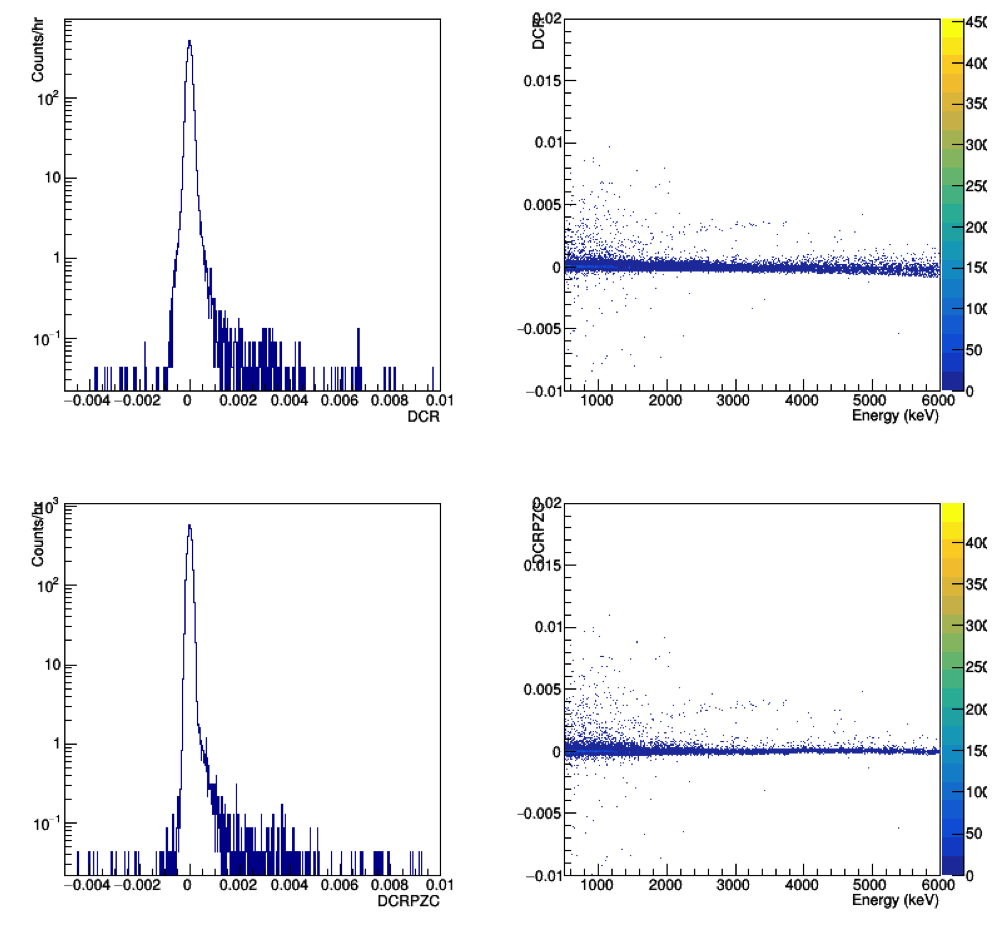
\includegraphics[width=.8\textwidth]{/Users/jgruszko/Documents/Thesis/Plots/Ch3/TUBE_DCRPZ}
 %\caption[A comparison of v1.0 and v2.0 of the DCR analysis, in the TUBE system]{Preliminary tests of version 2.0 of the DCR parameter, in the TUBE scanning system. {\it Top:} The version 1.0 DCR distributions, for energies between 1 and 6~MeV. {\it Bottom:} The version 2.0 DCR distributions. The two-point slope DCR parameter is calculated and applied after a pole-zero correction is used to de-convolve the electronics response function. The use of version 2 leads to a narrower bulk-event distribution, particularly at energies above 3 MeV, where muons and multisite events dominate.} 
% \label{fig:TUBE_v2}
%\end{figure*}

%%%%%% This is a results section %%%%%%
\section{\MJ\ Analysis}
\subsection{Efficiencies}
In each channel, the average acceptance for single-site events (after data-cleaning) in the Compton continuum region, taken to be from 1\,MeV to 2.38\,MeV, is set to match the quoted acceptance of the cut. For instance, {\tt dcr99} has average bulk acceptance of 99\%, as nearly as is allowed by the finite statistics of the sample used to set the cut. 

The true acceptance for the \nonubb\ region is calculated from that energy region directly, also using calibration data, due to the energy non-linearity effect, as discussed above. It is given in Table~\ref{tab:DS_efficiencies} for each of the data sets.  

\subsection{Uncertainties}

\begin{table}[]
\centering
\begin{tabular}{l l l l l l l}
Data Set & $\epsilon_{ROI}$ (\%) & $\sigma_{PS}$ (\%) & $\sigma_{stab}$  (\%) & $\sigma_{stat}$  (\%) &$\sigma_{tot}$ (\%) \\ 
\hline
DS0  & 98.1  &  0.8  &    &  0.1  &  0.9 \\   
DS1  & 95.6  &  1.1  &    &  0.1  &  1.1 \\
DS2  & 98.6  &  0.9  &    &  0.2  &  1.0 \\
DS3  & 99.1  &  0.9  &    &  0.1  &  0.9 \\
DS4  & 98.9  &  1.2  &    &  0.1  &  1.2 \\
DS5a  & 92.1  &  0.7  &    &  0.3  &  0.8 \\
DS5b  & 95.8  &  1.4  &    &  0.2  &  1.4 \\
\end{tabular}
 \caption[\nonubb\ efficiency and uncertainties in the \MJ\ \DEM]{\nonubb\ efficiency and uncertainties, given for high gain channels in each data set. DS5 was split into DS5a and DS5b because the presence of elevated electronic noise in DS5a (due to known ground loop problems) drastically reduced the effectiveness of the DCR cut in these runs.} 
 \label{tab:DS_efficiencies}
\end{table}

As discussed, the pulse shape systematic uncertainty and uncertainty due to cut instability dominate, with the statistical uncertainties contributing about 0.2\% and the energy scale uncertainty contributing negligibly. The uncertainties for each data set are given in Table~\ref{tab:DS_efficiencies}. 

\subsection{DCR Validation in Low-Background Data}

\begin{figure*}[]
 \centering
 \begin{subfigure}[t]{0.45\textwidth}
   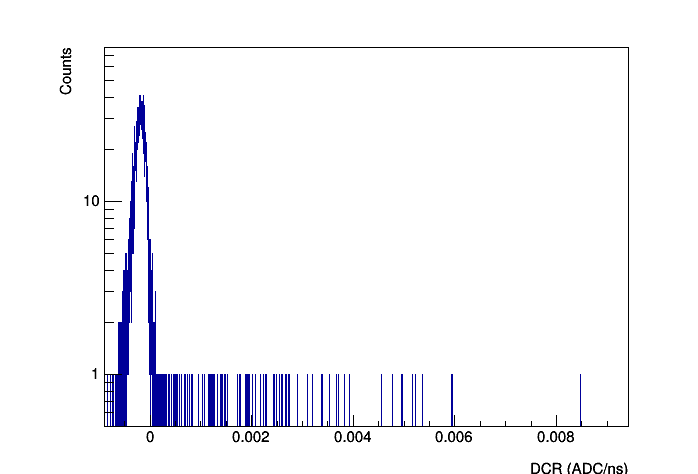
\includegraphics[width=\textwidth]{/Users/jgruszko/Documents/Thesis/Plots/Ch3/DS3_DCR_HG}
    \caption{The DCR distribution.}
    \label{fig:DS3_DCR}
  \end{subfigure}
\hfill
 \begin{subfigure}[t]{0.45\textwidth}
   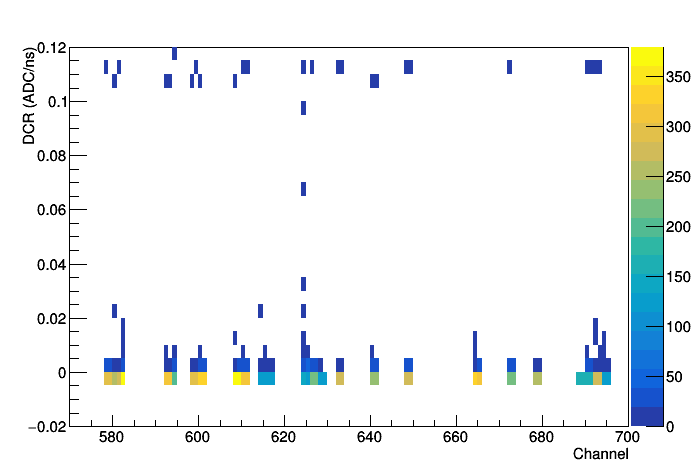
\includegraphics[width=\textwidth]{/Users/jgruszko/Documents/Thesis/Plots/Ch3/DS3_DCRvCh}
    \caption{The DCR distribution for each channel.}
    \label{fig:DS3_DCRvCh}
  \end{subfigure}
   ~
 \begin{subfigure}[t]{0.45\textwidth}
   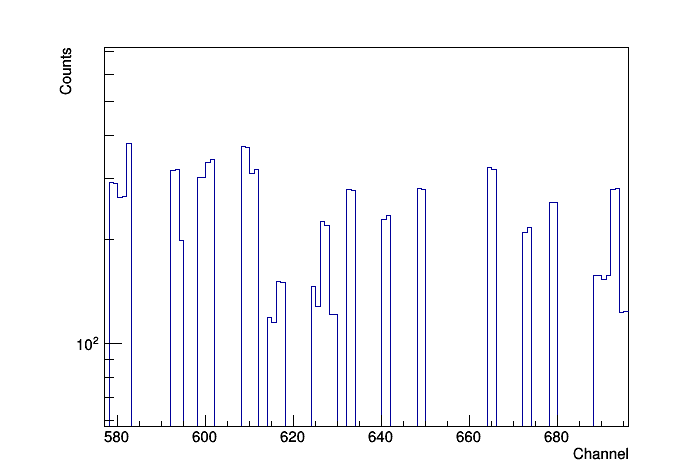
\includegraphics[width=\textwidth]{/Users/jgruszko/Documents/Thesis/Plots/Ch3/DS3_events_byCh}
    \caption{The number of events remaining after the DCR cut, in each channel.}
    \label{fig:events_byCh}
  \end{subfigure}
\hfill
  \begin{subfigure}[t]{0.45\textwidth}
   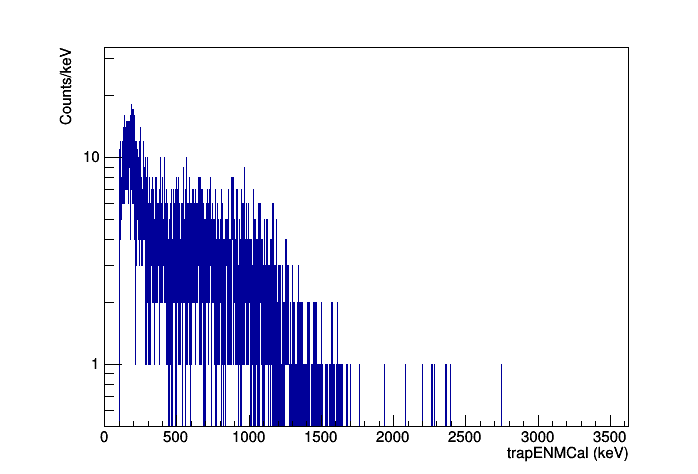
\includegraphics[width=\textwidth]{/Users/jgruszko/Documents/Thesis/Plots/Ch3/DS3_E_HG}
    \caption{The spectrum after the DCR cut is applied.}
    \label{fig:DS3_E_HG}
  \end{subfigure}
   ~
  \begin{subfigure}[t]{0.45\textwidth}
   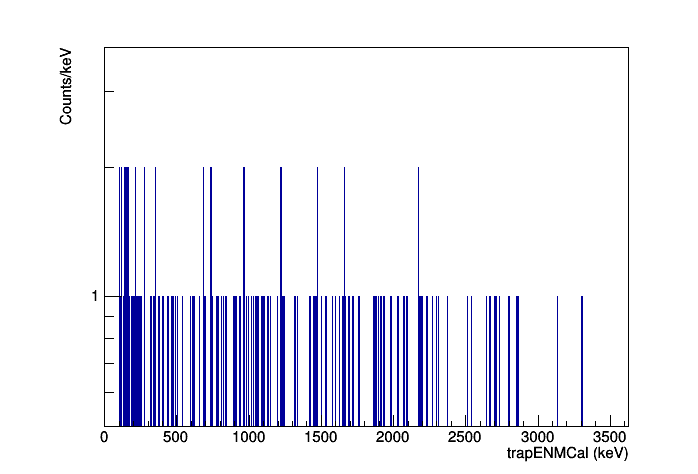
\includegraphics[width=\textwidth]{/Users/jgruszko/Documents/Thesis/Plots/Ch3/DS3_Ecut_HG}
    \caption{The spectrum of events cut by DCR.}
    \label{fig:DS3_Ecut_HG}
  \end{subfigure}
\hfill
     \begin{subfigure}[t]{0.45\textwidth}
   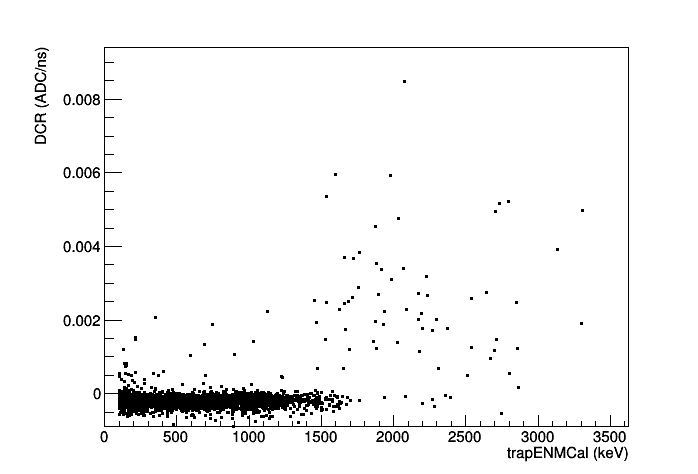
\includegraphics[width=\textwidth]{/Users/jgruszko/Documents/Thesis/Plots/Ch3/DS3_DCRvE_HG}
    \caption{The DCR vs. energy distribution.}
    \label{fig:DS3_DCRvE_HG}
  \end{subfigure}
  \caption{The results of DCR validation for DS 3 high gain channels.}
  \end{figure*}
  
 \begin{figure}[t]
   \centering
   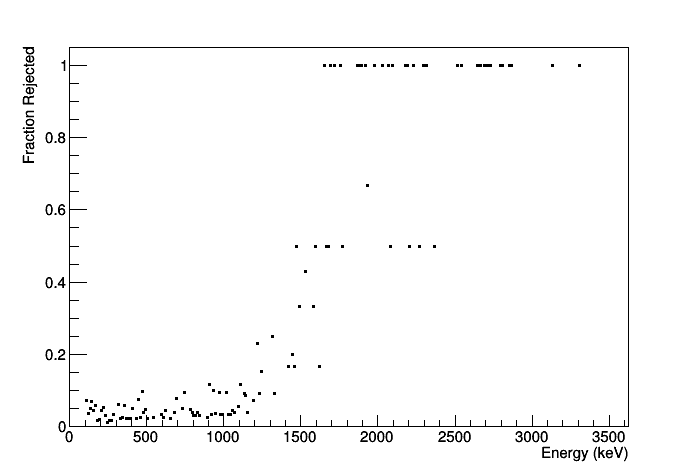
\includegraphics[height=3in]{/Users/jgruszko/Documents/Thesis/Plots/Ch3/DS3_DCRrej}
    \caption{The DCR rejection fraction as a function of energy, in DS 3 high gain channels.}
    \label{fig:DS3_DCRrej}
  \end{figure}

The DCR in each background skim data set is checked using a dedicated validation script, which is used to check for channels in which the DCR parameters are not being applied correctly, unexpected energy dependence, and other errors in the DCR parameters.  The validation script is applied first to the open data, and then, after unblinding, to the remaining data. This script produces the following plots:
\begin{itemize}
\item The DCR distribution in the channel: It should have an roughly gaussian shape, with a high-DCR tail extending to the right. The peak should be centered at a DCR value less than 0. See Fig.~\ref{fig:DS3_DCR}. If a channel does not have a DCR cut available, a sharp (single-bin-width) spike will appear at 0 along with the gaussian for the correctly calculated parameters. 
\item The DCR distribution for each channel: Each distribution should be peaked just below 0, with a tail extending to high-DCR values. All events appearing at 0, or a peak appearing in a different location, are indications of errors in the DCR parameters. See Fig.~\ref{fig:DS3_DCRvCh}.
\item The number of events retained by the DCR cut in each channel: All bins should be similar in height. See Fig.~\ref{fig:events_byCh}.
\item The energy spectrum after the DCR cut is applied: It should resemble the \twonubb spectrum at energies above 500\,keV, with no large dips at any particular energies. There should be few events remaining above 1.8\,MeV. See Fig.~\ref{fig:DS3_E_HG}.
\item The energy spectrum of the events removed by the DCR cut: It should be roughly flat, with a small rise at low energy. See Fig.~\ref{fig:DS3_Ecut_HG}.
\item The DCR vs. energy distribution of events: Most events above 1.8\,MeV should have visibly high DCR. Below 1.5\,MeV, most events should have DCR below 0. See Fig.~\ref{fig:DS3_DCRvE_HG}.
\item The DCR rejection efficiency as a function of energy, in 10\,keV bins: It should be at or near 1 in most bins above 1.8\,MeV, and fall to approximately 10\% (i.e. the set cut bulk-acceptance) at energies below 1\,MeV. See Fig.~\ref{fig:DS3_DCRrej}.
\end{itemize}

If no anomalies or major instabilities (see above) are found, the DCR cut is ready to be used in spectral analysis. 


 
 
% ========== Chapter 5
 
\chapter {The TUBE Scanning System}\label{ch:TUBE_exp}

\section{Introduction}
As previously discussed in Ch.~\ref{ch:DCR}, $\alpha$ particle backgrounds originating on or near the passivated surface of \ppc\ detectors are a major contributor to the \MJ\ \DEM\ background spectrum, but can be identified effectively via a delayed-charge recovery (DCR) pulse-shape discriminator. While \thtte\ source calibrations and \twonubb\ events can be used to estimate the DCR acceptance of bulk events, a sample of known passivated-surface $\alpha$ events are needed to estimate the $\alpha$ rejection efficiency of the analysis. Such measurements can also be used to estimate the $\alpha$ background spectral shape both before and after the DCR cut, allowing the construction of an accurate background model for the \DEM. 

Given that the weighting potential near the passivated surface varies drastically with radius (see Fig.~\ref{fig:wp_z0}), the energy lost to delayed charge in these events, and therefore the reconstructed energy of the events, is also expected to vary with radius. Similarly, the rate of charge re-release and amount of charge released, which combine to produce the DCR parameter value, are also expected to vary with radius. These variations lead to an radially- (and therefore energy-) dependent $\alpha$ rejection efficiency. The form of the DCR and energy variation depends on the mechanism of charge delay and/or loss, including whether only electrons or both holes and electrons are affected, and whether surface-charge transport or charge-trapping (followed by re-release into the bulk) near the passivated surface is primarily responsible for the observed delayed-charge effect. 

To study these effects, a collimated \am\ source was used to scan PONaMA-1, a \ppc\ detector with the same geometry as the enriched detectors currently operating in the \MJ\ \DEM. Data was taken at with the source incident at positions spanning nearly the entire diameter of the passivated surface. 

\section{Experimental Setup}
\subsection{PONaMa-1}
The detector chosen to be scanned was PONaMa-1 (serial number TP42486A), a test-run detector produced by ORTEC using natural-abundance germanium. Its production process was identical to that used for the enriched detectors in the \DEM, and its geometry is similar to that of those detectors. Its properties are given in Table~\ref{tab:PONaMA_specs}. 

\begin{table}[]
%\begin{tabular}{p{4cm} | l}
\centering
\begin{tabular}{p{5cm} | l}
\hline
\multicolumn{2}{c}{PONaMA-1 Properties} \\
\hline
Diameter & 68.9\,mm \\ 
Height & 52.0\,mm \\ 
Dimple Diameter & 3.2\,mm \\
Dimple Depth & 2.0\,mm \\
Capacitance & 1.8\,pF \\
Depletion Voltage & 1850\,V \\
Leakage Current & 10\,pA \\
Resolution at 1332\,keV \newline (Measured at ORTEC) & 1.99\,keV \\
\end{tabular}
\caption{Dimensions and operating parameters of the PONaMa-1 \ppc\ detector.}
 \label{tab:PONaMA_specs}
\end{table}

\begin{figure*}[p]
 \centering
  \begin{subfigure}[]{\textwidth}
  \centering
 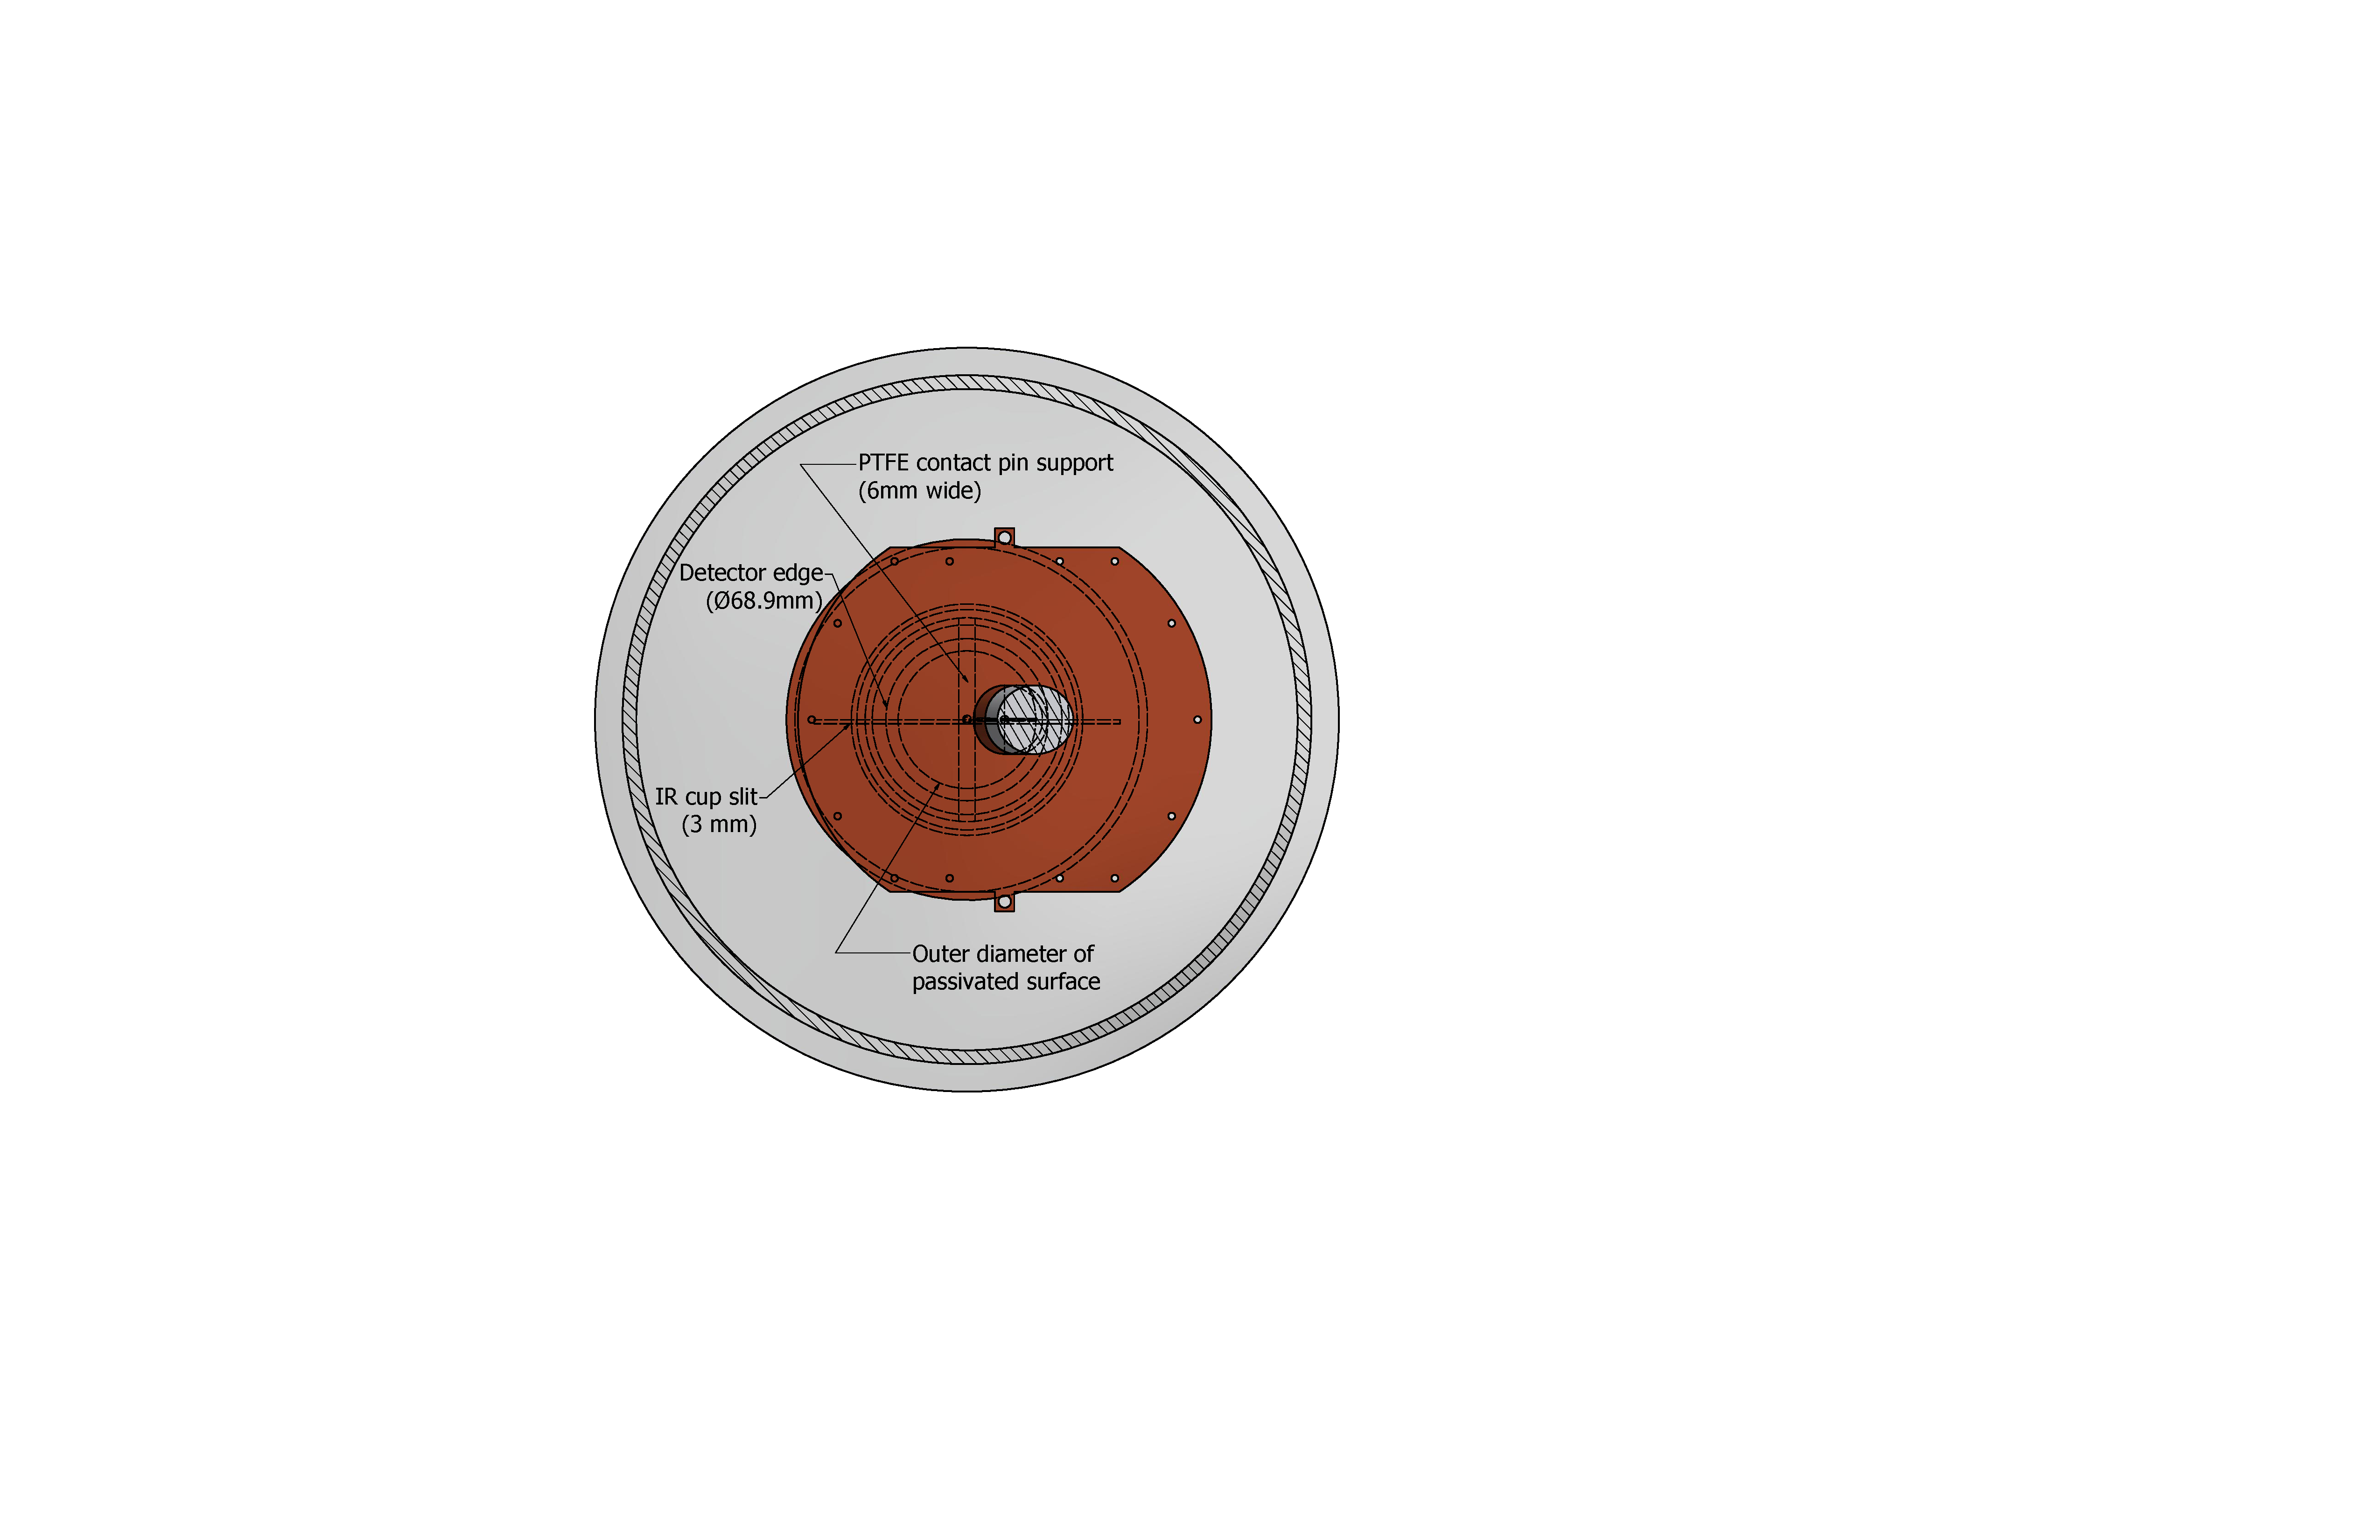
\includegraphics[height=.35\textheight]{/Users/jgruszko/Documents/Thesis/Images/Ch5/TUBE_assembly_top}
 \label{fig:TUBE_top}
\end{subfigure}
  ~
  \begin{subfigure}[]{\textwidth}
   \centering
 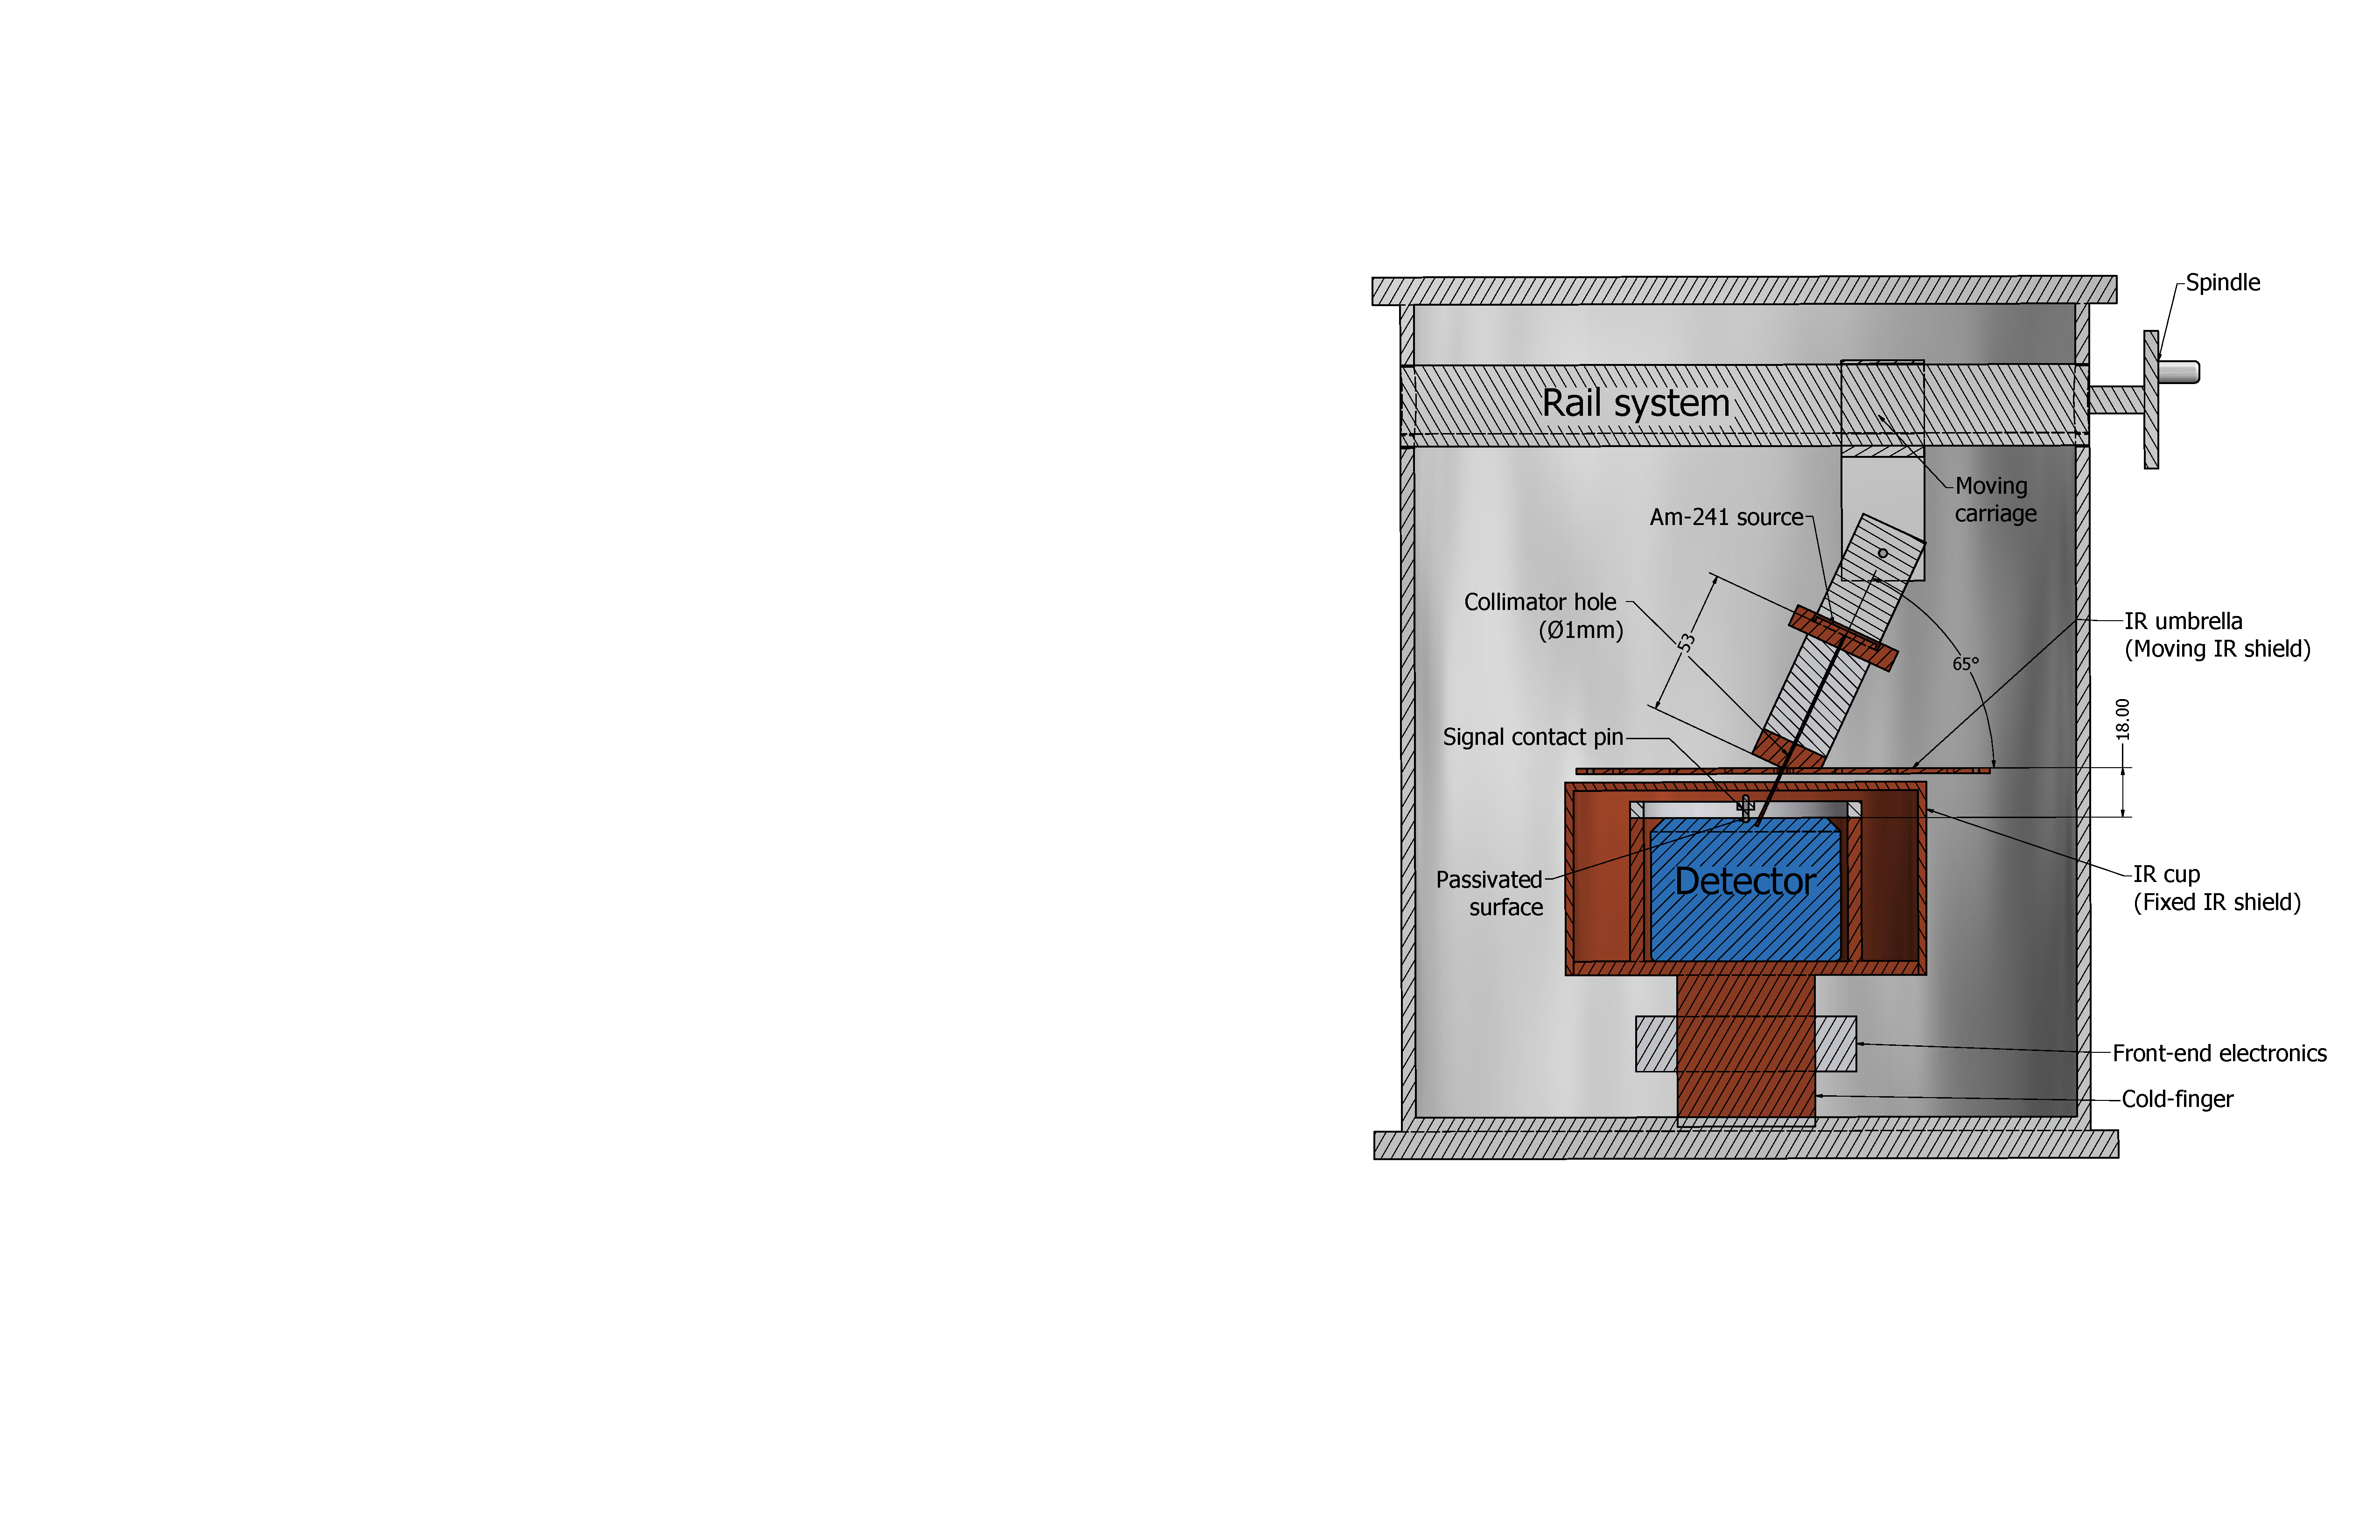
\includegraphics[height=.55\textheight]{/Users/jgruszko/Documents/Thesis/Images/Ch5/TUBE_assembly_side}
 \label{fig:TUBE_side}
 \end{subfigure}
\caption[A diagram of the TUBE scanner]{Simplified top {\it (top)} and bisected views {\it (bottom)} of the TUBE scanner, showing key dimensions. The thermal braids connecting the IR umbrella to the IR cup and the mylar covering of the IR umbrella are not shown. Details of the detector cup, front-end electronics, and cold-finger are also removed for clarity.}
\label{fig:TUBE_views}
\end{figure*}

\subsection{The TUBE Scanner}
The TUM (Technical University of Munich) Upside-down BEGe (TUBE) scanner is a custom-built cryostat first made to study the backgrounds in GERDA due to surface interactions on the p+ electrode and groove of Canberra BEGe \ppc\ detectors. It allows a \ppc\ detector to be installed ``upside-down," with the passivated surface facing upwards, so that the surface may be scanned with a collimated source. The scanner consists of three main parts, seen in Fig.~\ref{fig:TUBE_views}: the cryostat, detector holder, and collimator assembly. 

The cryostat is made from a stainless steel tube with top and bottom flanges, with a vacuum feed-through that allows the cryostat cold-finger and signal electronics (from a Canberra vendor cryostat) to be inserted. A rail system is mounted at the top of the vessel, with a rotational feedthrough on the sidewall that allows the collimator radial position to be changed while the system is under vacuum. The collimator assembly is mounted to the carriage of this rail system, which has a pitch corresponding to 1.5\,mm of travel for every turn of the spindle. Ultra-high vacuum in the vessel is achieved using a turbomolecular pumping stand with a diaphragm forepump, connected to the system by Viton-sealed flanges. The measurements described here were taken with the pump in continuous operation, though the cooled system can retain pressures of around 1E-5\,mbar even after eight hours without pumping. 

The detector is mounted in a modified version of the original TUBE copper holder, adapted for the dimensions of PONaMA-1 by the addition of teflon shims. This holder was made by adapting the vendor-cryostat detector mount, and houses the front-end electronics. Contact with the p+ electrode is made via a spring-loaded contact pin, held in a narrow Teflon\textsuperscript\textregistered holder that also provides routing for the signal cable, which runs from the contact pin to the front-end electronics. This holder creates a 6-mm ``blind spot" on the detector surface that cannot be scanned. See Figs.~\ref{fig:scan_coords} and ~\ref{fig:TUBE_photo}. 

\begin{SCfigure}
\centering
 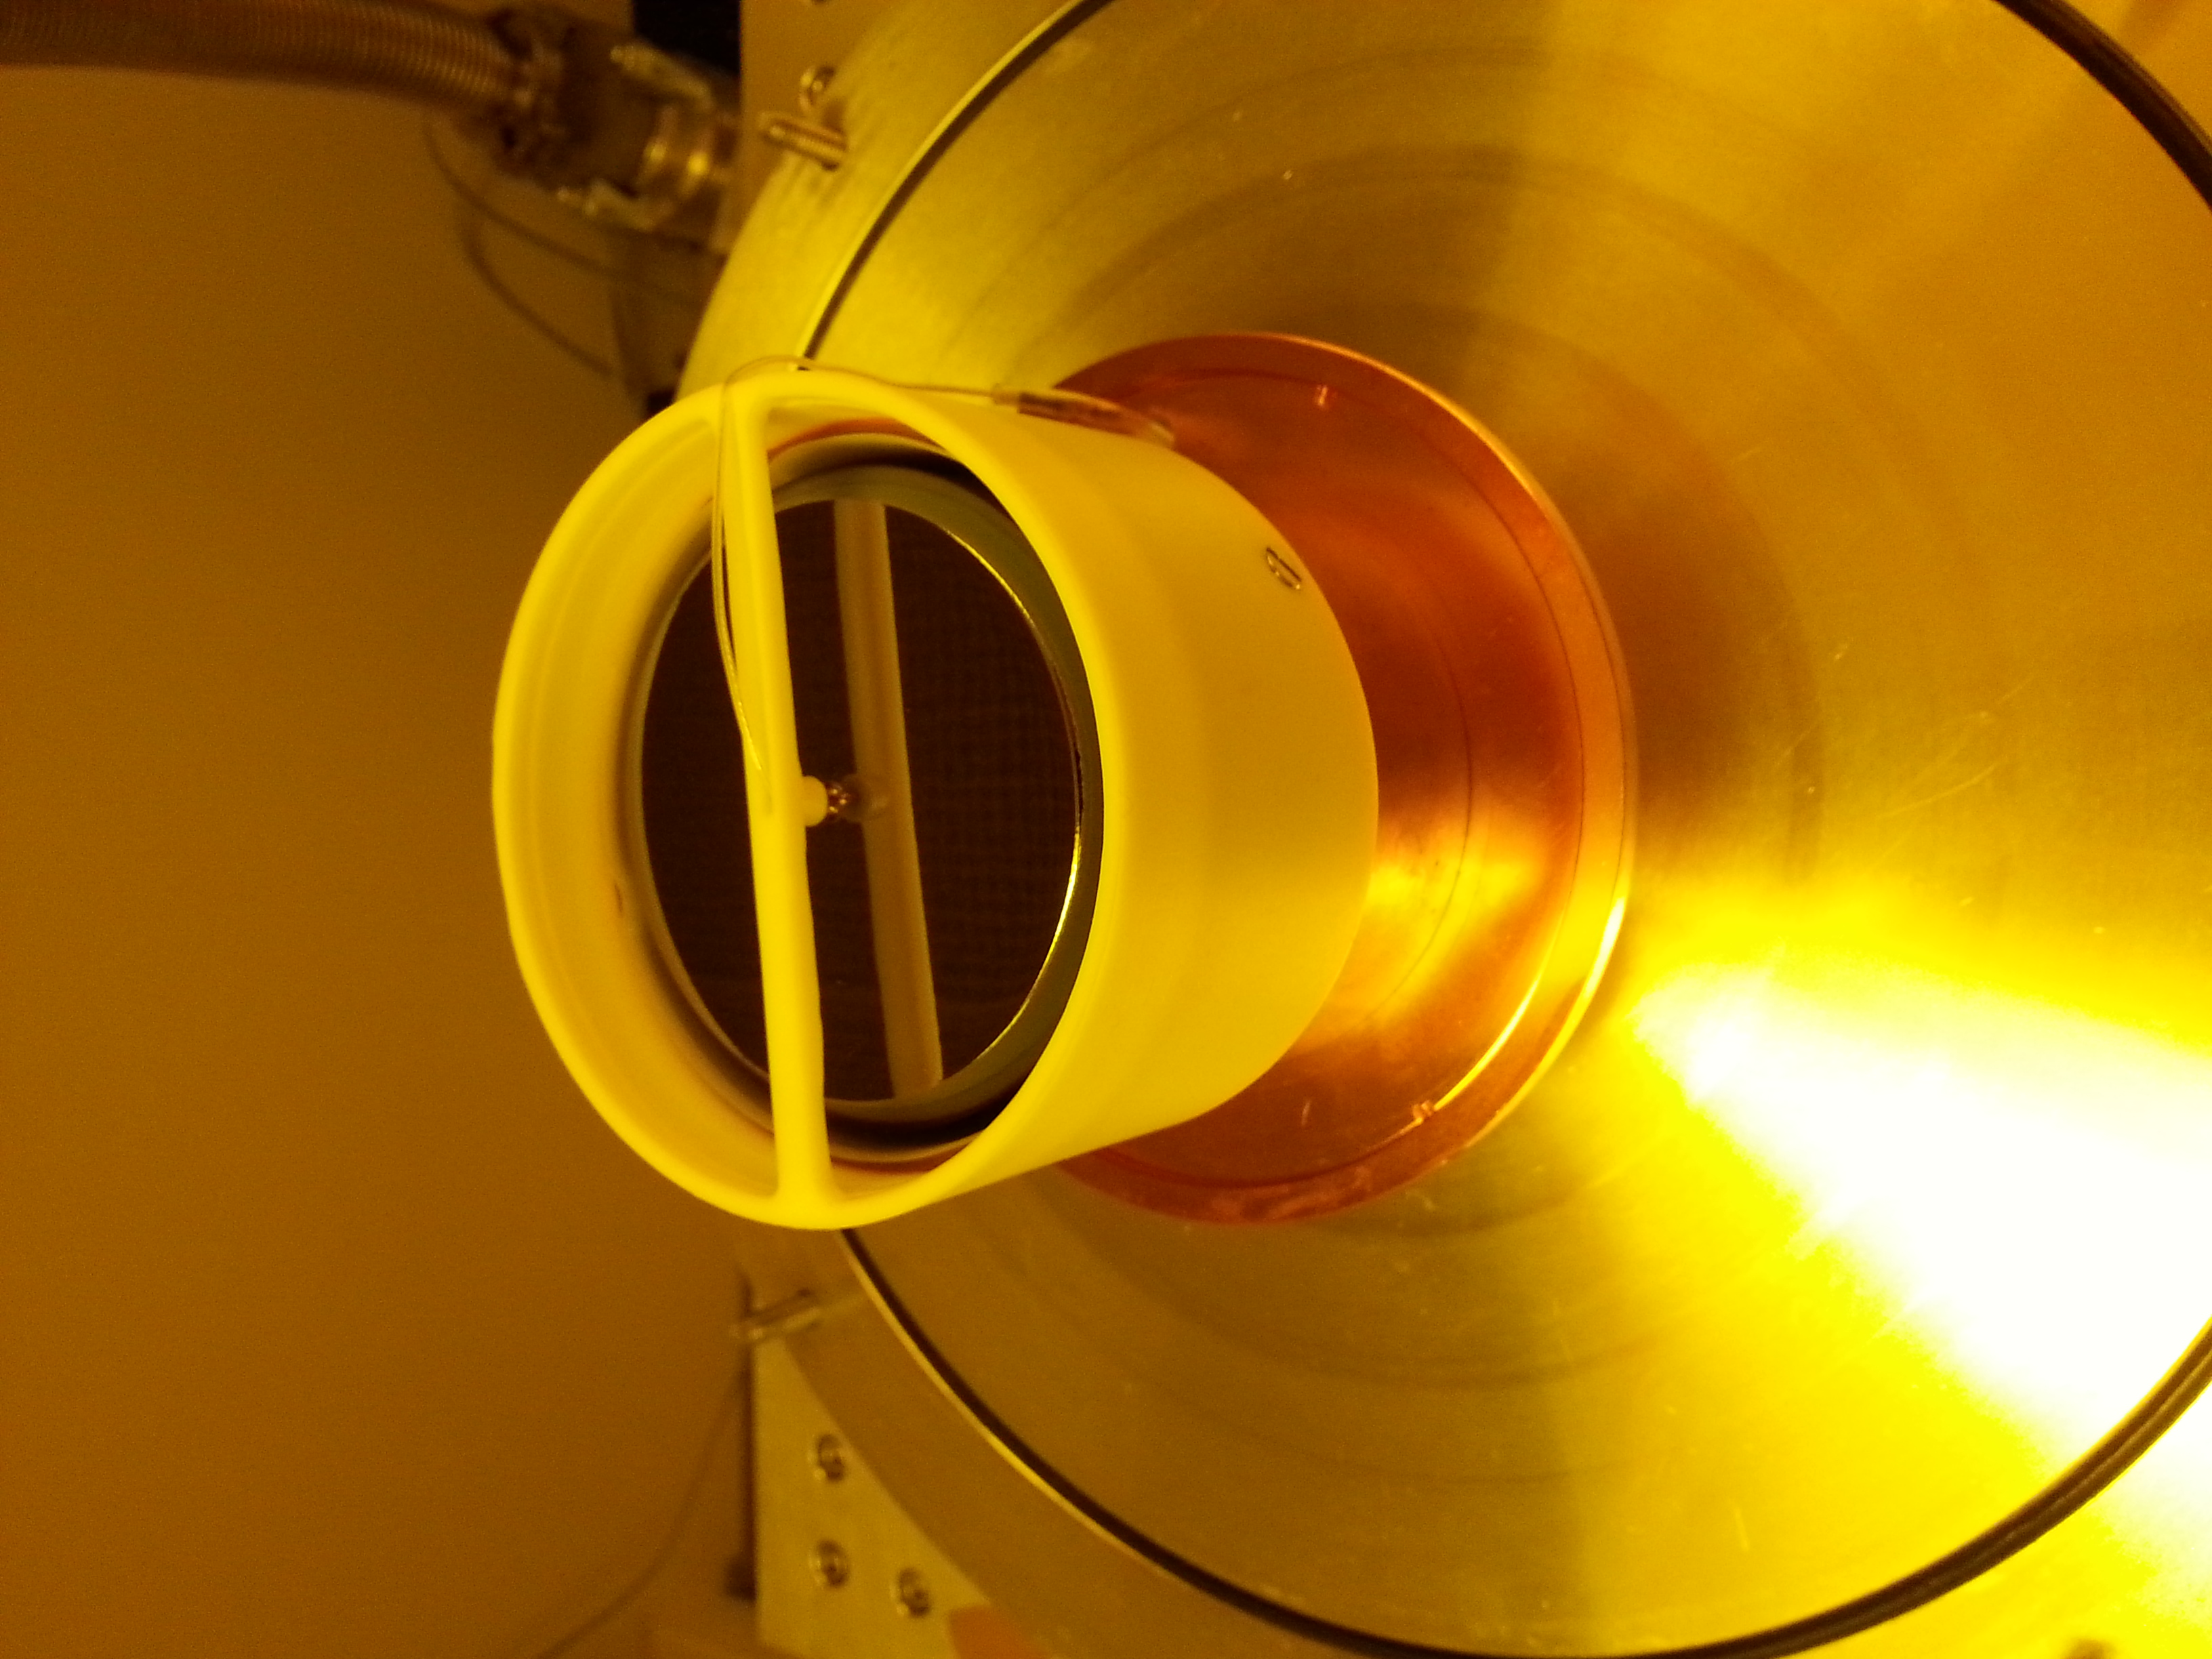
\includegraphics[height=3in, angle=270, origin=c]{/Users/jgruszko/Documents/Thesis/Images/Ch5/TUBE_detector}
 \caption[A photo of PONaMa-1 installed in the TUBE detector cup]{A photo of PONaMa-1 installed in the TUBE detector cup. The contact pin, visible at the center of the detector, is held by the Teflon\textsuperscript\textregistered\ crossbar, with the signal cable running along the top.} 
 \label{fig:TUBE_photo}
\end{SCfigure}

This assembly is housed inside a copper IR-shield (called the ``IR cup") with a 3\,mm slit running along its diameter. This slit defines the axis that is scanned along, as the source beam shines through it onto the detector surface. See Fig.~\ref{fig:TUBE_views}. 

Further IR-shielding, required due to the high IR-shine susceptibility of the large passivated surface of ORTEC \ppc\ detectors, was added for use with PONaMA-1. It is provided by a copper ``IR umbrella" shield, mounted on the tip of the collimator and moving along with the source. This shield, which minimizes the IR-shine onto the passivated surface through the slit of the IR cup, is thermally grounded to the IR cup via two flexible high-thermal-conductivity copper braids. The dimensions of the IR umbrella were subject to the existing constraint of the TUBE cryostat chamber diameter; therefore, it does not completely cover the IR cup slit at all scanning positions. This leads to variation in the detector leakage current as the collimator is moved along the surface. The top face of the IR umbrella is covered with several layers of insulator-backed Mylar\textsuperscript\textregistered, to minimize its radiative heat-load. The IR umbrella and mylar sheets have a 3\,mm diameter hole to allow the source beam to penetrate. 

\begin{figure}[]
 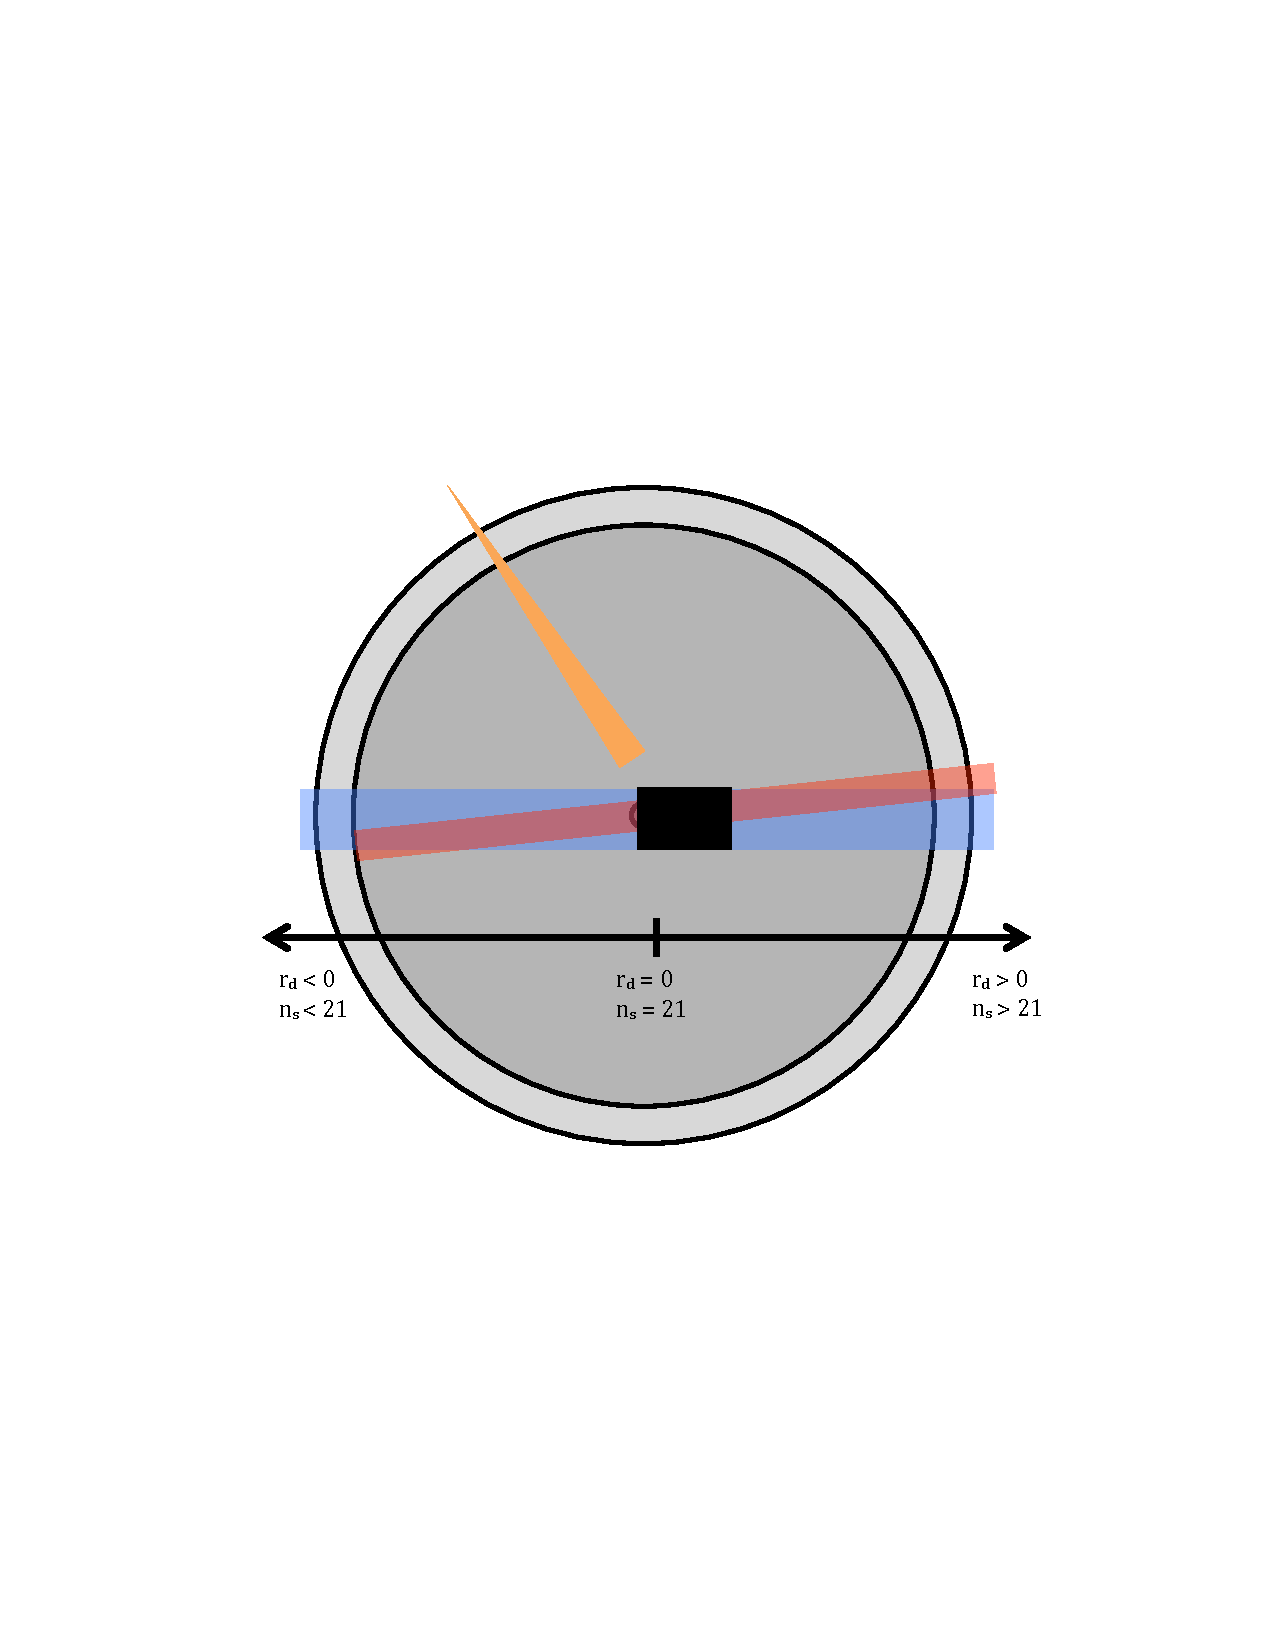
\includegraphics[width=1.0\columnwidth]{/Users/jgruszko/Documents/Thesis/Images/Ch5/coord_system}
 \caption[A diagram showing the accessible regions of the detector surface and the coordinate system of the TUBE scanner]{A diagram showing the accessible scanning regions and the coordinate systems used to describe the source position. The dark gray and light gray regions represent the passivated surface and edge of the n+ contact surface, respectively. The gold triangle represents the source beam, which forms a $66\degree$ angle to the negative r axis. The blue region represents the portion of the detector visible through the IR cup slit, and the red region is the path traced out by the source beam. Notice that due to the misalignment of the two axes, only the region of their overlap can be scanned. The black region is the inaccessible ``blind spot" due to the contact-pin holder. It occludes all but one edge of the p+ contact region, which spans the region from $r_d = -1.6$\,mm to $r_d = 1.6$\,mm. Dimensions not to scale.} 
 \label{fig:scan_coords}
\end{figure}

A photo of the TUBE scanning system (Fig.~\ref{fig:TUBE_photo}) shows the configuration of the IR umbrella, thermal grounding braids, and Mylar\textsuperscript\textregistered insulation. 

\begin{figure}[t]
\centering
 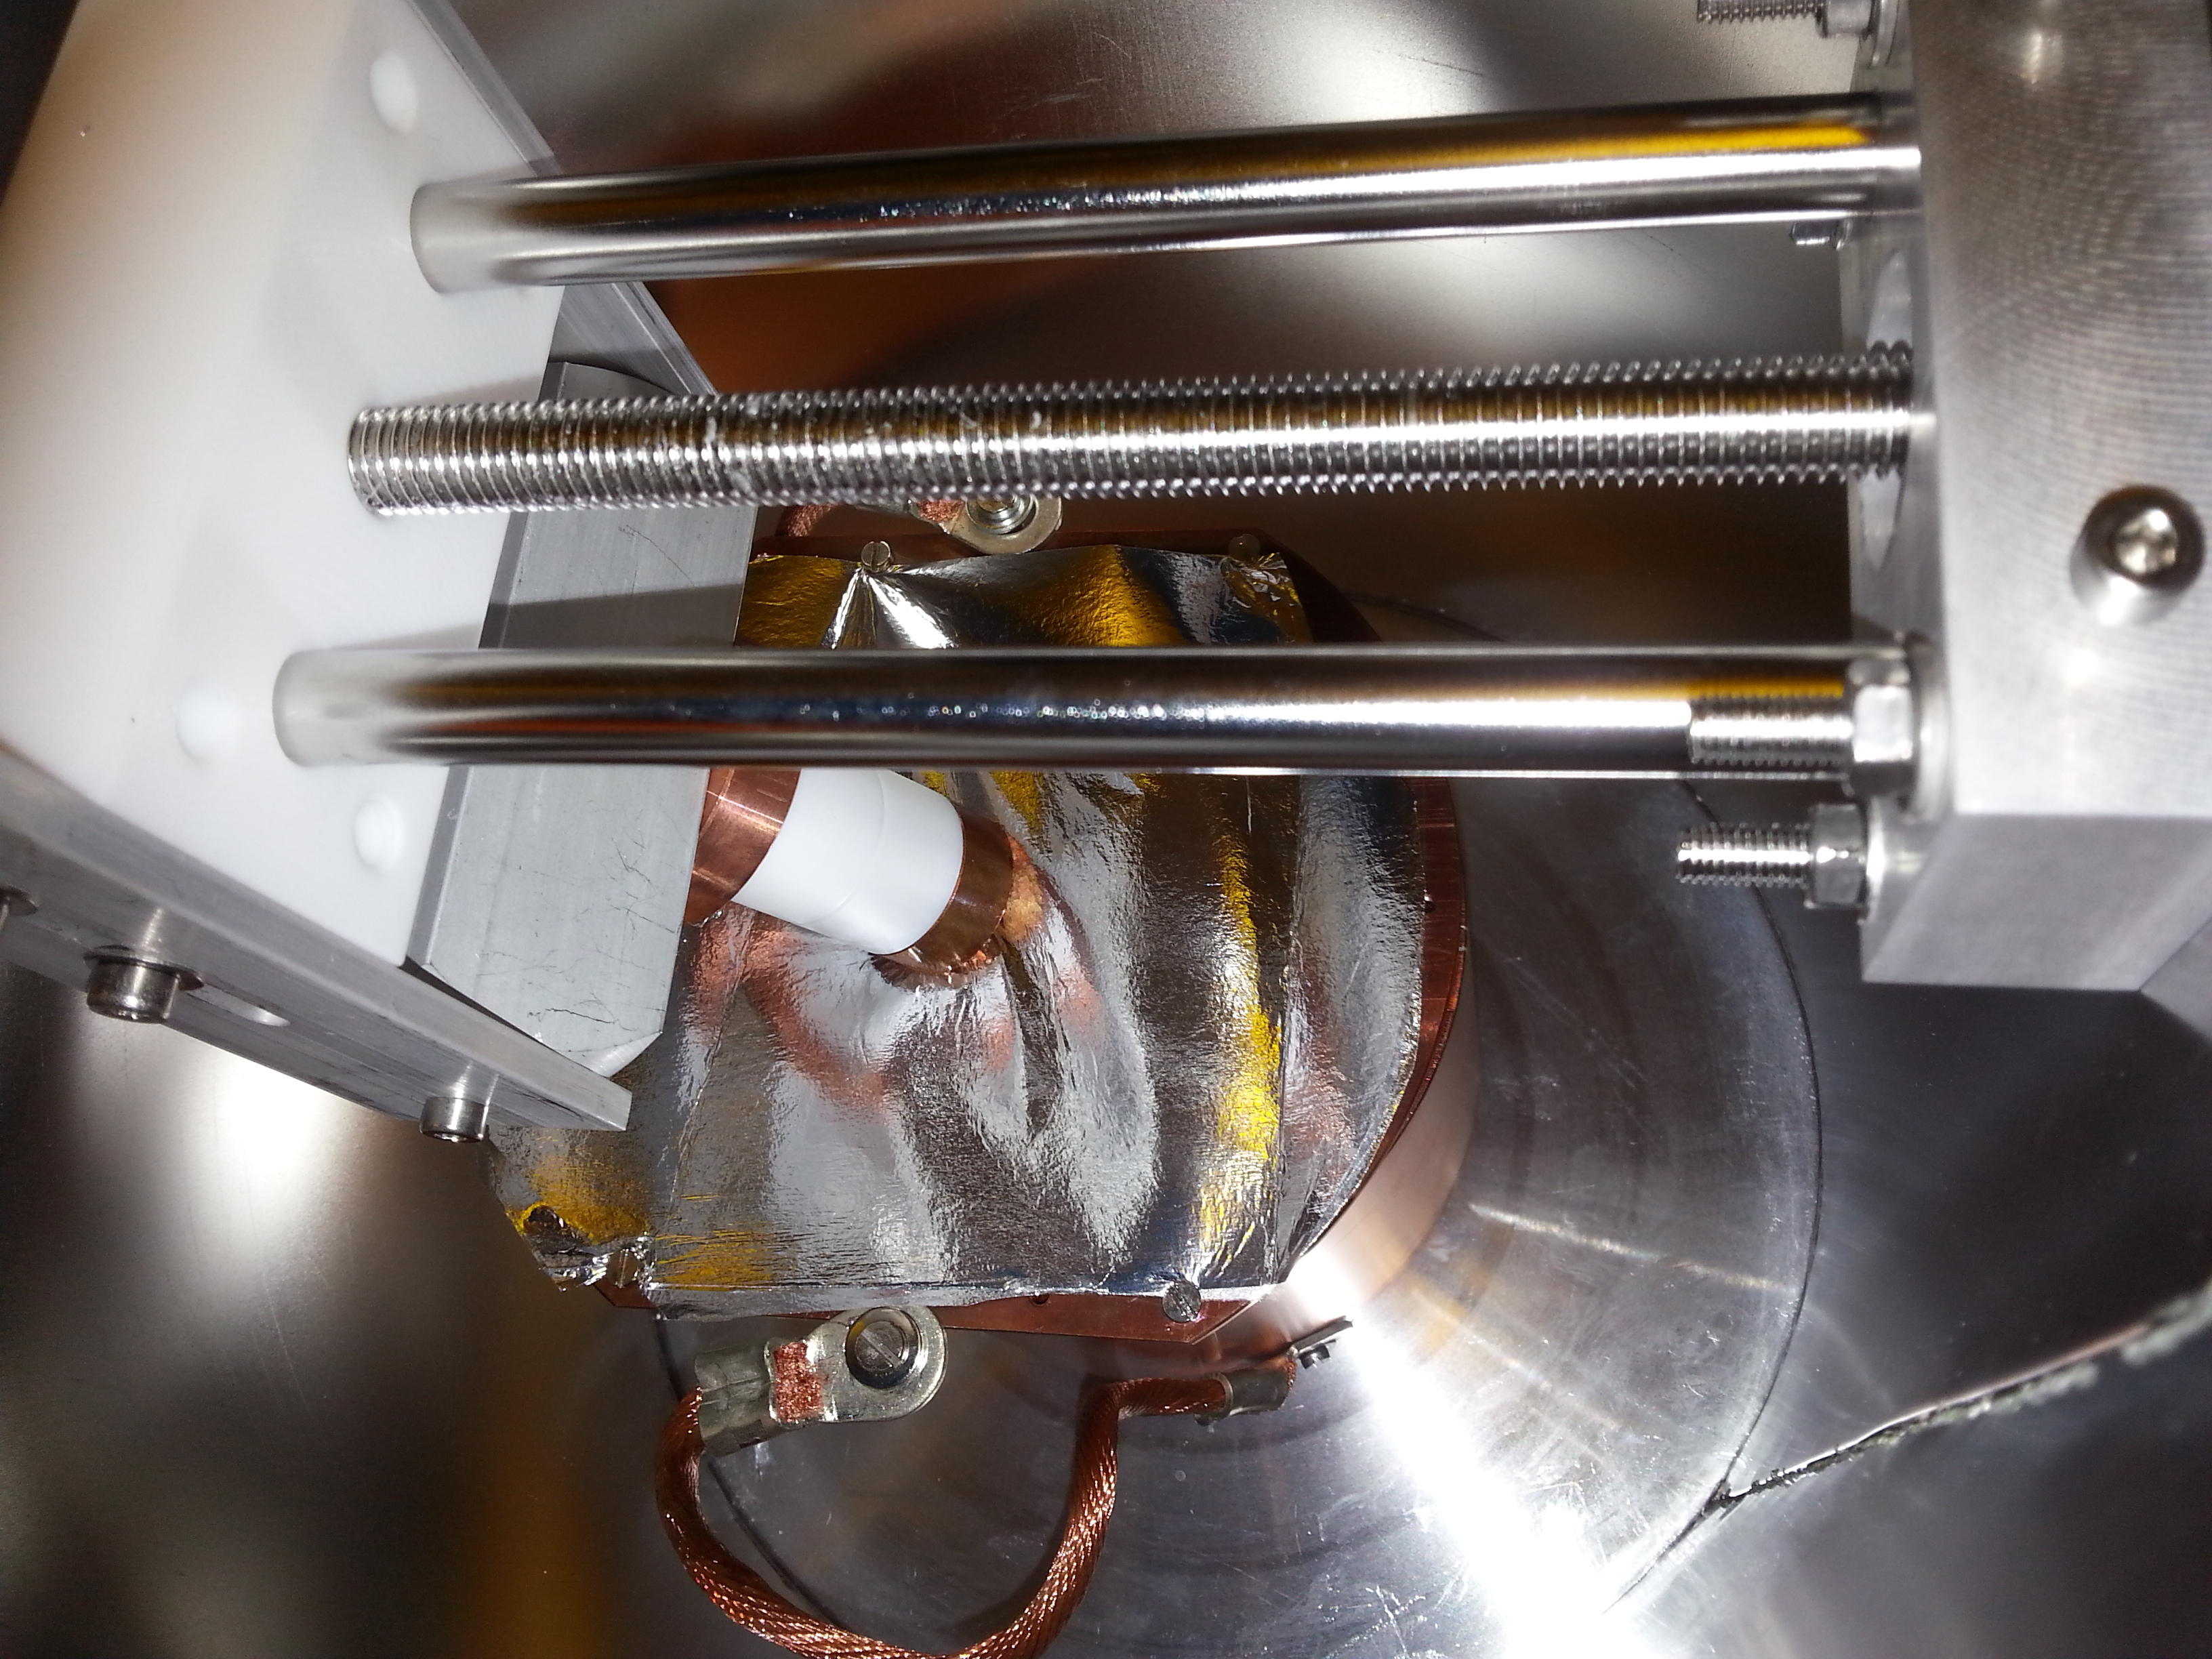
\includegraphics[height=4in]{/Users/jgruszko/Documents/Thesis/Images/Ch5/TUBE_photo_top}
 \caption[A photo of the inside of the TUBE scanner]{A photo of the inside of the TUBE scanner. The moving carriage and rail system is at the top, with the source and collimator suspended from it. The IR umbrella is suspended from the collimator tip, and is cooled via the thermal grounding braids, one of which is visible at the bottom of the photo.} 
 \label{fig:TUBE_photo}
\end{figure}

\subsection{\am\ Source and Collimator Properties}

The collimator has an overall length of 53\,mm, and is suspended from the carriage of the rail system. The source is housed in a copper holder with a 1\,mm diameter collimating hole. The beam then passes through a teflon and aluminum tube, with a collimating hole of 3\,mm in diameter, that thermally isolates the source holder, carriage, and rail system from the IR umbrella. The collimator assembly ends in a copper tip with a 1\,mm diameter collimator hole, which is chamfered to create a source-beam incidence angle of $66.8\degree$ to the horizontal plane. In the course of mounting the collimator to the rail system, this angle may change by up to $2.3\degree$ in either direction without impeding the movement of the source. For these measurements, the incidence angle is taken to be $65\degree$, as discussed in Sec.~\ref{ssec:geometry}. The spot size of the source on the detector surface is approximately 1.8\,mm in diameter. 

The \am\ source used was a 40\,kBq alpha spectrometry source provided by Eckert \& Ziegler Nuclitec GmbH, with product code AMR14. It is an open source, with the radionuclide deposited onto a 7\,mm-diameter spot of a stainless steel disc. This minimizes energy degradation, giving an expected full width at half maximum for the 5.486\,MeV $\alpha$ peak of less than 20\,keV. In the expected event rate calculation, we assume that the radionuclide is deposited with equal density over the entire 7\,mm spot.

Given the source strength and collimator geometry, an activity of 18\,mBq (i.e. 65 events/hour) is expected at the detector surface. 84.8\% of events, corresponding to an activity of 15\,mBq (54 events/hour) should include a 5.486\,MeV $\alpha$ emission. Another 13.1\% of events include a 5.443\,MeV $\alpha$ emission \cite{nudat_Am}. If the energy resolution of the detector is sufficiently reduced by interactions in the passivated surface, these peaks will be indistinguishable, and 98\% of the total activity will lie in the observed peak. 

\subsection{Muon Veto System}
The expected vertical flux of cosmic ray $\mu$ with energy over 1\,GeV is 1\,cm$^{-2}$\,min$^{-1}$ at sea level for a horizontal detector \cite{PDG2014}. Therefore the expected rate of high energy $\mu$ in the TUBE system detector is approximately 620\,mBq (2240 events/hour), far overwhelming the expected $\alpha$ event rate. An active muon veto system is used to reduce cosmic $\mu$ background rate. The veto system used consists of a 50\,cm by 50\,cm plastic scintillator panel and photomultiplier tube (PMT), placed on top of the cryostat. 

\subsection{Data Aquisition}
High voltage to PONaMA-1 was suppled by a CAEN N1471HA module. The detector was first operated at 950\,V of bias, 100\,V above the observed depletion voltage; ultimately, the bias was raised to 1050\,V to eliminate pinch-off. A Canberra Model 2002 Spectroscopy Preamplifier was used, with the low gain (100\,mV/MeV) setting in place. 

The veto system PMT was operated at a 1000\,V bias, and amplified using a Canberra Model 2025 AFT Research Amplifier, with a gain of x20 and a shaping time of .5$\mu$s. 

Data from both PONaMA-1 and the muon veto system were taken with a Struck SIS3302 digitizer, sampling at 100\,MHz. The digitizer and readout are controlled using ORCA (Object-oriented Real-time Control and Acquisition) \cite{ORCA}.

\section{Measurements Taken} \label{sec:measurements}
\subsection{As-Built Geometry} \label{ssec:geometry}
Several elements of the TUBE scanner geometry are determined at the moment of assembly, and are subject to human error. In particular, both the total vertical distance between the collimator tip and detector surface and the source beam incidence angle are approximate. Given the observed positions of the detector edges, the vertical spacing is thought to be 22\,mm (rather than the expected 18\,mm), and the angle of incidence is thought to be 65$\degree$ (rather than the expected 66.8$\degree$). 

With these as-built dimensions, the mapping from number of turns of the spindle, which is used to describe the data sets, to source spot position on the detector surface is given by $r_d = (n_s-20)(1.5\,mm)$, where $n_s$ is the number of turns and $r_d$ is the distance from the point contact on the surface of the detector. Negative and positive radii are defined as shown in Fig.~\ref{fig:scan_coords}, with 0 at the center of the p+ contact. The region between $r_d = -1$\,mm and  $r_d = 7$\,mm is occluded by the contact-pin and PTFE contact-pin holder, and cannot be scanned. The center of the point-contact is occluded by the contact pin itself. 

In the course of the measurements, it was discovered that the IR cup slit and scanning axis were misaligned. This led to a falling source rate at large-magnitude negative scanning radii, as seen in Fig.~\ref{fig:peak rate}. An additional slight sideways shift in the collimator mounting position (i.e. when aligned with the P-contact, the source shines slightly to one side of the IR-slit center line, rather than into the center of the P-contact), leads to a difference in the source obstruction at negative and positive radii. Based on the observed source rates and known geometry, the angular misalignment must be less than 2.5$\degree$, and the sideways misalignment must be less than 1\,mm. 

Hysteresis effects were observed in the source position, so an uncertainty of 0.75\,mm (corresponding to a 1/2 turn of the spindle) is assigned to all source positions. 

\subsection{Data Sets}
Data were taken at all integer-turn positions for at least 24 hours. Each of these run sets, taken without changing the source position or operating conditions, is grouped into a data set. Several multi-day runs were also taken to study the stability of the system. In those cases, multiple data sets cover the span of time, with each data set corresponding to approximately one day of run time. Scanning positions were repeated non-contiguously to study the effect of the source position hysteresis and the long-term stability of the DCR parameters. Measurements were taken at half-turn positions in the vicinity of the p+ contact and at the edges of the passivated surface.  

%\input{data_set_list.tex}

\section{Data Processing Scheme}
\subsection{Analysis Chain}
The data were analyzed using a modified version of the \MJ\ processing stream. Runs are limited to half an hour in duration and 2\,GB in file size. In practice, $\alpha$ source and background runs are half an hour long, and thorium calibration runs (whether taken with a \thtte\ or \thttt\ source) are shorter.

Each half-hour run is processed independently until the final step of processing. Using the Majorcaroot (MJOR)  and OrcaRoot software packages, the raw ORCA output files are converted into ROOT output files, which contain {\tt TTree}s of ORCA output parameters encapulated in Majorana Gerda Data Objects (MGDO) classes. Included in each run's {\tt TTree} are the raw waveforms collected by the digitizer. These waveforms are 30\,$\mu$s long and sampled at 100\,MHz, with the trigger appearing about 10\,$\mu$s after the start of the waveform. These waveforms are packaged into ``events," which contain all waveforms that triggered within a 10\,$\mu$s window. If a cosmic ray muon triggers both the veto panel PMT and germanium detector, for instance, the event will contain two waveforms. The resulting files are referred to here as ``built" data files.

The built data is then processed using the Germanium Analysis Toolkit (GAT) software package. At this processing step, each waveform has a variety of filters (such as baseline removal, pole-zero correction, etc.) and parameter calculators applied to it. Multiple waveforms in a given event are also processed in conjunction to give parameters such as multiplicity. The energy calibration (determined as described below) is applied during this stage of processing. All of the resulting values are saved to the ``reconstructed" data files, which do not contain the waveforms themselves. 

\begin{table}[]
\begin{tabular}{p{2in}| p{4in}}
\hline
\multicolumn{2}{c} {Selected Reconstructed Data Parameters} \\
\hline
Name & Description \\  \hline
{\tt run} & Run number \\
{\tt channel} & Channel (Ge or PMT) \\
{\tt timestamp} & Digitizer timestamp at time of trigger (in 10\,ns units)\\
{\tt startTime} & Start time of run (in UTC) \\
{\tt stopTime} & Stop time of run (in UTC) \\
{\tt m} & Multiplicity of event \\
{\tt pileUpWFsnRisingX} & Number of rising threshold crossings of pile-up trap. filter\\
{\tt trapEMPZ} & Maximum of baseline-removed, pole-zero corrected, trapezoidal-filtered waveform. \\ 
{\tt trapEMPZCal} & Calibrated version of the above, used for Ge energy determination. \\
{\tt onboardE} & Digitizer trap. filter energy, optimized for PMT energy determination\\
{\tt blrwfSlope} & Tail slope of baseline-removed waveform \\
{\tt mjdblrwfSlope} & Tail slope of MJD-emulating baseline-removed waveform \\
{\tt blrpzcwfSlope} & Tail slope of baseline-removed pole-zero-corrected waveform \\
{\tt TSCurrent200Max} & Current filter maximum \\
\end{tabular}
 \label{tab:GATparams}
\end{table}

A summary of the parameters saved at this stage is given in Table~\ref{tab:GATparams}. Baseline removal is applied by subtracting the average value of the first 500 waveform samples from each sample of the waveform. The pole-zero correction applied uses the decay constant $\tau = 44.224\,\mu$s, found by fitting to the decay of 1000 pulses in a calibration run from the first calibration data set taken. The trapezoidal filter used for energy reconstruction has an integration time of 8\,$\mu$s and a collection time of 3\,$\mu$s. A second trapezoidal filter, with integration time of 0.5\,$\mu$s and collection time of 0.3\,$\mu$s, is used to tag pile-up events. A one-sided trapezoidal filter, with integration time of 200\,ns and peaking time of 10\,ns, is used to calculate the current 'A' used in the determination of A vs. E (see A vs E unidoc for details). 

Three varieties of the waveform tail slope, which will be used to determine the DCR parameters, are saved. The values are the result of a two-point slope calculation, using the average value (in ADC) of the waveform in a 1\,us region for each of the points. All three varieties use the region starting 2\,us after the 97\% rise point of the waveform as the first point. The {\tt blrwfSlope} and {\tt blrpzcwfSlope} use the final 1\,us of the baseline-removed waveform as their second span. For the latter, pole-zero correction is applied before measuring the slope. The {\tt mjdblrwfSlope} parameter emulates the waveforms collected in \MJ\ data sets that do not use multi-sampling (MJD Data Sets 0, 1, and 3-5). For this parameter, the baseline-removed waveform is cut to have only 2016 samples, removing the final 10\,$\mu$s of decay tail. Then the final 1\,us of the shortened waveform is used as the second region. See Fig.~\ref{fig:tailslope}.


\begin{figure*}[]
 \centering
 %\begin{subfigure}[]{\columnwidth}
 \centering
 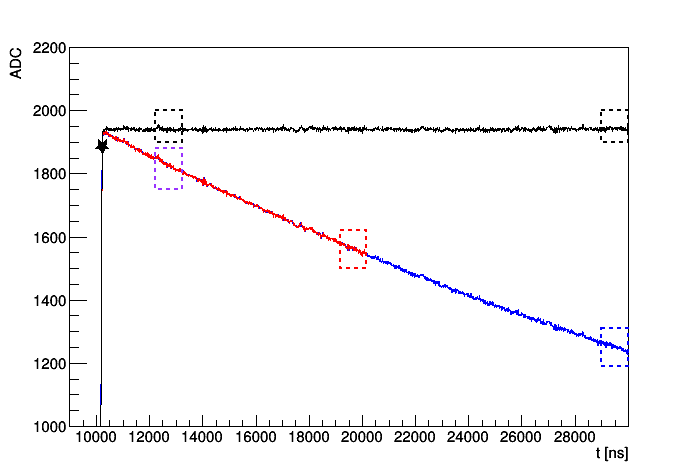
\includegraphics[height=2in]{/Users/jgruszko/Documents/Thesis/Plots/Ch5/tailslope_params_zoom_noTitle.png}
 \caption[A sample TUBE waveform, with indicated tail slope measurement points]{Sample 2614\,keV waveform, with the points needed to calculate various tail slope parameters. The star indicates the 97\% rise point of the pulse. The blue waveform has had its baseline removed; the slope between the averages in the violet and blue dotted regions is the {\tt blrwfSlope}. The red waveform has had its final 10\,us chopped following baseline removal to emulate singly-sampled MJD waveforms; the slope between the averages in the violet and red dotted regions is the {\tt mjdblrwfSlope}. The black waveform has had pole-zero correction applied after baseline removal; the slope between the averages in the black dotted regions is the {\tt blrpzcwfSlope}.} 
 \label{fig:tailslope}
% \end{subfigure}
~
% \begin{subfigure}[]{\columnwidth}
  \centering
 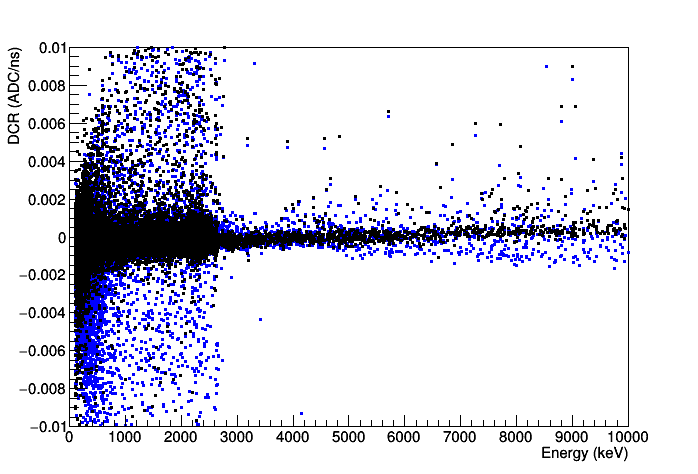
\includegraphics[height=2.5in]{/Users/jgruszko/Documents/Thesis/Plots/Ch5/dcr90_comparison_highE.png}
 \caption[A comparison of v1.0 ({\tt dcr90}) and v2.0 ({\tt dcrpzc90}) of the DCR analysis in the TUBE system]{A comparison of {\tt dcr90} and {\tt dcrpzc90} in single-site calibration events (from calibration data set 8) after the muon veto is applied. {\tt dcr90} falls and degrades in resolution at energies over 4\,MeV. Though {\tt dcrpzc90} rises slightly with increasing energy, likely due to a small change in the pole-zero decay constant $\tau$ between calibration data set 1 and 8, the effect is minimal compared to the broadening of {\tt dcr90}.} 
 \label{fig:dcr_dcrpzc_comparison}
% \end{subfigure}
\end{figure*}

In the final step of processing, GAT is used to combine about 24 hour's worth of consecutive runs into a skimmed data set. An offline energy threshold is applied to both the germanium and PMT data to reduce the number of noise events in the data set, and these thresholds are used to calculate a ``clean" multiplicity that excludes events below the analysis threshold. 

Other high-level parameters (i.e. those that require calibrated energy as an input value) are also calculated at this stage. These include A vs. E, which is the multi-site event discriminator used in this work (see A vs. E unidoc), A/E, a multi-site discriminator that is used to identify near-point-contact events, and the DCR parameters, described below. 

\subsection{DCR Parameters}
For a detailed discussion of the procedure used to calculate DCR parameters, see DCR unidoc (citation). 

Four types of DCR parameters are calculated for each PONaMA-1 waveform. For each of the parameters, versions are saved with 99\% and 90\% bulk acceptance. The {\tt dcr90} and {\tt dcr99} parameters are calculated using the waveforms after baseline-removal, with no other filters applied. The {\tt mjddcr90} and {\tt mjddcr99} parameters are derived from the MJD-emulating waveforms, which have only a 10\,$\mu$s decay tail, instead of a 20\,$\mu$s one. The are provided as a point of comparison to study the effectiveness of the DCR analysis in the \MJ\ data sets that do not use multisampling. Both of these sets of DCR parameters are calculated using the procedure described in the DCR unidoc. 

The final 2 sets of DCR parameters, {\tt dcrpzc90} and {\tt dcrpzc99}, are calculated using the baseline-removed waveform after pole-zero correction. This eliminates the need for the step in which the tail slope parameter is projected onto the energy axis, and creates a DCR parameter that has no dependence on energy for high-DCR events, unlike the other DCR parameter values. The DCRPZC parameters are a measure of the amount of delayed charge collected in the first 20\,$\mu$s after the fast, bulk charges are collected. 

The {\tt dcrpzc90} ({\tt dcrpzc99}) parameter is calculated by finding the 90\% (99\%) acceptance value of {\tt blrpzcwfSlope} for single-site non-muon events with energies between 1\,MeV and 2380\,keV, and subtracting this value from {\tt blrpzcwfSlope}. Therefore, 90\% (99\%) of bulk events should have {\tt dcrpzc90} ({\tt dcrpzc99}) $< 0$.  

The DCRPZC parameters are the most appropriate set to use when comparing TUBE results to waveform simulations, which do not include pole-zero decay. This version of the DCR analysis also performs better with respect to muon events; bulk events have consistent average DCRPZC even at high energy, while DCR degrades in resolution and falls off at energies above 4\,MeV. See Fig.~\ref{fig:dcr_dcrpzc_comparison}. Except for cases in which a direct comparison of TUBE results to \MJ\ data is required, DCRPCZ is used in this work. Ultimately, we plan to move to a similar analysis for the \MJ\ data as well, as described in the DCR unidoc. 

Additionally, normalized versions of DCRPZC, {\tt dcrpzc90norm} and {\tt dcrpzc99norm}, are calculated to correct for small instabilities in gain, PZ-decay constant, and noise in the system. To create these parameters:
\begin{itemize}
\item The {\tt blrpzcwfSlope} distribution of single-site calibration events with $1\,MeV< E < 2380\,keV$ is fit with a gaussian peak, the fit range of which is set to exclude the high-DCR tail). 
\item The centroid of the fit is subtracted from {\tt blrwfSlope}.
\item The 90\% (99\%) acceptance value is found as described above.
\item The shifted {\tt blrpzcwfSlope} values are normalized by the cut value.
\end{itemize}

Therefore, 90\% (99\%) of bulk events should have {\tt dcrpzc90norm} ({\tt dcrpzc99norm}) $< 1$, and value of these parameters is insensitive to changes in the gain of the system, unlike the unnormalized DCRPZC parameters.  

\section{Detector Performance}
\subsubsection{Energy Calibration}
Energy calibration using the GAT Multipeak Fitter (see energy Unidoc) is applied to each data set. Fourteen peaks in the spectrum ranging in energy from 295\,keV to 2614\,keV are fit with a gaussian peak, a low energy tail, a high energy tail (which fits to small values, in general), a step (which is centered at the gaussian centroid), and a linear or quadratic background (depending on the expected shape of the continuum in the peak region).

Comparing the resulting fit to a fit in which the peak positions were allowed to float, it was found that a linear calibration curve gave a poor fit to the peak positions in the spectrum. The residuals appeared to lie on a quadratic curve, with the 2614\,keV peak position being underestimated by up to 0.8\,ADC (corresponding to approximately 1\,keV). 

The fit was improved by the addition of a quadratic component to the peak position function (see Fig.~\ref{fig:calib_residuals}). I.e., the uncalibrated peak position is given by:
$$E_{ADC} = p_0 + p_1E_{keV} + p_2E_{keV}^2,$$
where $p_2$ is positive. With this change, the peak position residuals are generally less than 0.4\,ADC and are evenly distributed about 0, though some non-linearity remains, likely due to digitization effects. 

\begin{figure*}[]

 \centering
 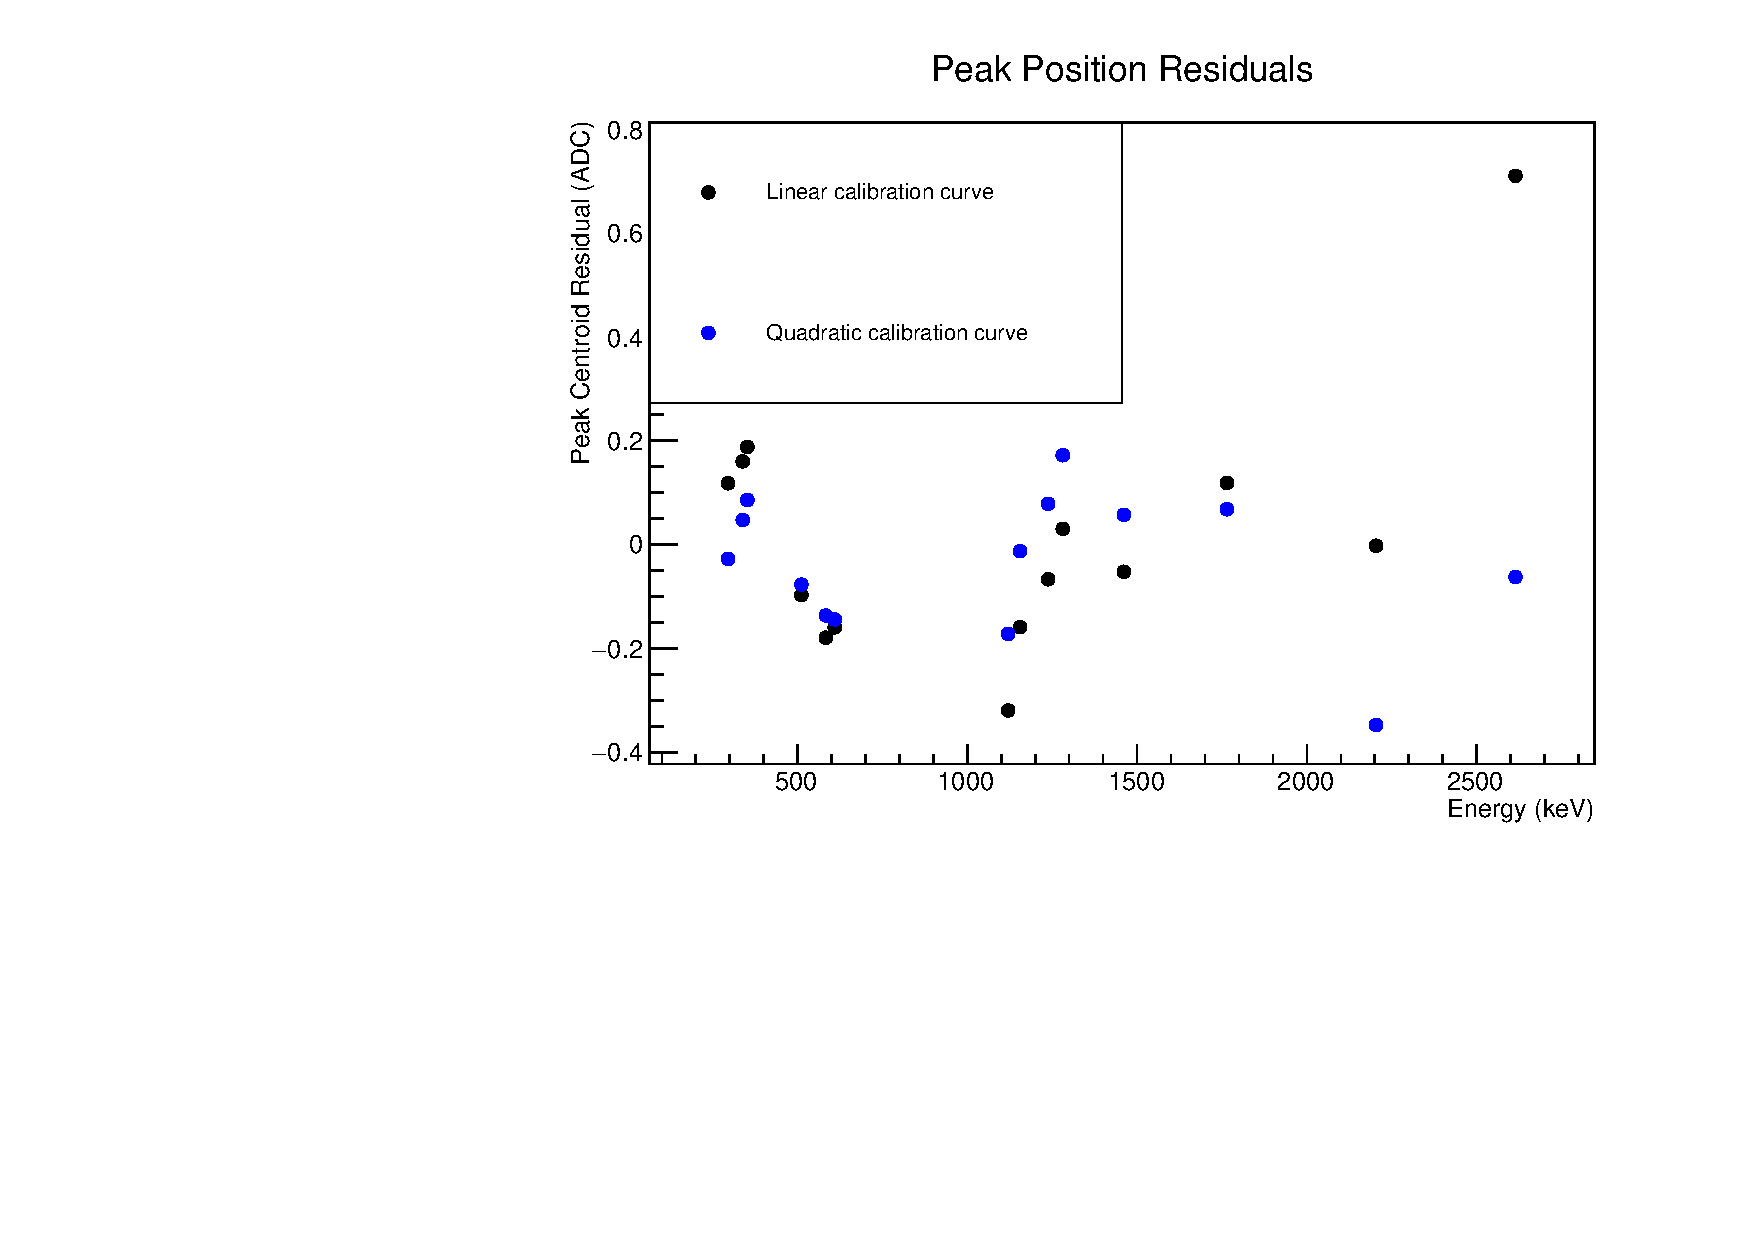
\includegraphics[height=3in]{/Users/jgruszko/Documents/Thesis/Plots/Ch5/residuals_comparison}
 \caption[The residuals of calibration peak positions]{The residuals of calibration peak positions. The entire spectrum was first fit with the peak positions (in ADC) restricted to lie either on a linear (in black) or quadratic (in blue) function of energy (in keV), and then fit with the peak positions allowed to float.} 
 \label{fig:calib_residuals}

 \centering
 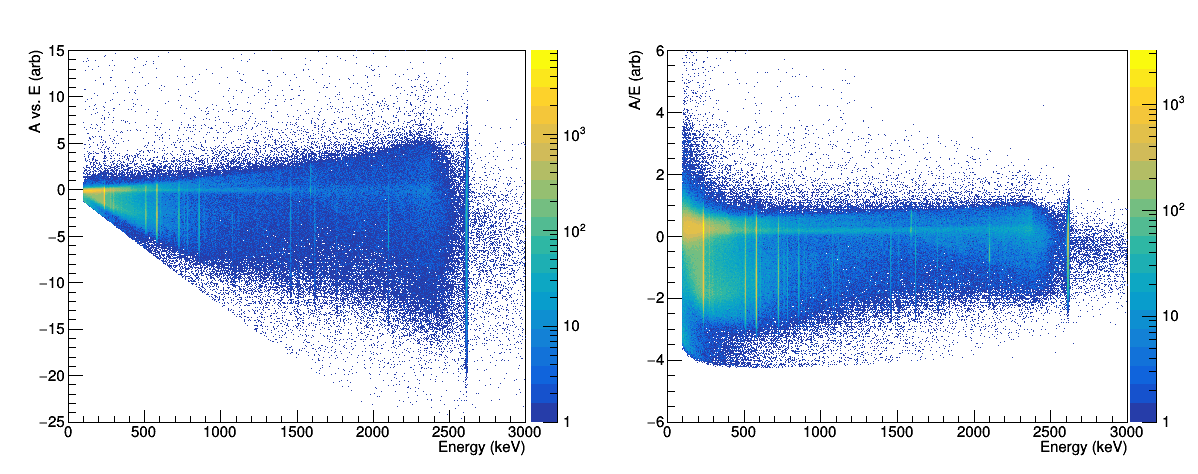
\includegraphics[width=\textwidth]{/Users/jgruszko/Documents/Thesis/Plots/Ch5/avse_aenorm_calibDS8.png}
 \caption[A comparison of A vs. E and A/E in calibration events]{A comparison of A vs. E {\it (left)} and A/E {\it (right)} in calibration events (from calibration data set 8) after the muon veto is applied. The color scale indicates the number of events. Near point-contact events have energy-dependent values of A vs. E, as seen in the sloped upper edge of the A vs. E distribution when it is drawn with respect to energy, but have energy-independent values of A/E. Therefore, A/E is used to identify near-point-contact events.} 
 \label{fig:avse_aenorm_comparison}
\end{figure*}

\subsubsection{Energy Stability}
Given the high room background rates, it is possible to calibrate every data set independently. The energy stability within data sets is measured by calculating the position of the 2614\,keV peak in ADC for each data set by applying the appropriate calibration constants, and then calculating the absolute value of the shift between consecutive data sets. The average shift is found to be $0.68\pm0.60$\,ADC, corresponding to $0.92\pm0.81$\,keV at the 2614\,keV peak. 

All shifts in the energy scale had less than a 2\,ADC effect on the position of the 2614\,keV peak save for one, between runs 1638 and 1639, which led to a shift of 4\,ADC. This shift was large enough to require that a stability correction be applied in the pulse-shape discriminating parameters. See below. 

\subsubsection{Energy Resolution}
The average FWHM at the 2614\,keV peak is $3.2\pm0.6$\,keV. The gaussian component of the peak has an average standard deviation of $1.1\pm0.1$\,keV, which would correspond to an average FWHM of $3.0\pm0.3$\,keV. The remaining contribution is due primarily to the low-energy tail, with a minimal contribution from the high-energy tail. The average resolution curve of the gaussian component is given by:
$$\sigma = \sqrt{\num{2.79e-1}+\num{3.21e-4}\,E_{keV}+\num{2.84e-9}\,E_{keV}^2}$$

The resolution suffers due to the continuous operation of the turbopump attached to the TUBE cryostat, since microphonic noise is introduced into the system. However, it was determined that the resolution was satisfactory for these measurements, and that gaining added duty cycles by avoiding pumping between measurements was a higher priority than optimizing the energy resolution. 

\subsubsection{A vs. E}
The ``A vs. E" pulse shape discriminator is used to tag and eliminate multi-site events, as described in \cite{AvsE_unidoc}. The parameters for the cut are set using $^{228}$Th calibration runs; unlike the $^{232}$Th spectrum, the $^{228}$Th spectrum has no other spectral peaks near the 2614\,keV double-escape peak (DEP), at 1592\,keV.

The current is estimated through the use of a 200\,ns {\tt TSCurrent} filter, which performs a linear fit to a small range of the waveform. The energy estimator used, {\tt trapEMPZCal}, is described above. The process used to determine the correct parameters and calculate the efficiencies and uncertainties is exactly that used for the \MJ\ analysis, which is described in the unidoc. 

To correct for the gain and noise change that occurred following run 1639, the A vs. E parameters and results are calculated separately for these two run periods. See Table~\ref{tab:AEresults}. These cuts are set using calibration data sets 1 and 8, which are 17.9 and 2.9\,hrs in duration, respectively. 



\subsubsection{A over E}
Since the width of the distribution of ``A vs. E" estimator values depends on energy (see Fig.~\ref{fig:avse_aenorm_comparison}), it is a poor choice of parameter to describe the shape of the pulses from near-point-contact alpha events. Instead, we use ``A over E," the current discriminator normalized by the energy. Using this estimator, near-point-contact events appear in an energy-independent band at higher values than single-site events. 

The A/E parameters are determined: 
\begin{itemize}
\item ``A," the maximum current, is taken to be the maximum value of a 200\,ns {\tt TSCurrent} filter.
\item The ratio A/E is calculated for all events.
\item For each of eight spectral peaks with energies from 1000 to 2220\,keV, the mean A/E value is calculated.
\item A linear function in energy is fit to the mean A/E values. This energy correction is applied to all A/E values. 
\item The A/E cut value is chosen such that 90\% of events in the DEP are accepted, following statistical background subtraction (using the sidebands of the peak).
\item The cut value is subtracted from the energy-corrected A/E value to give the ``multi-site corrected A/E" (A/E$_{corr, MS}$).
\item The 99\% acceptance value of of A/E$_{corr, MS}$ is determined. This is the value that 99\% of events (whether multisite or single-site) with energies between 1\,MeV and 2630\,keV lie below. A/E$_{corr, MS}$ is normalized by this value.
\end{itemize}

Therefore, multi-site events are expected to have A/E $<0$, and single-site events will have $A/E>0$. The final normalization corrects for gain instability and changes in the noise of the system, and 99\% of calibration-run gamma events will have $A/E<1$. Near point-contact events will have $A/E \gg 1$. 
 
As for A vs. E, the A/E acceptance in the DEP and SEP are calculated using statistical background subtraction. The region from 1989\,keV to 2089\,keV, termed the \nonubb\ region, provides an estimate of the Compton continuum reduction provided by the cut. Again, a stability correction is applied after run 1639. See Table~\ref{tab:AEresults}. 

\begin{table}[t]
%\begin{center}
\centering
\begin{tabular}{l l r r r}
\hline
PSD & Run Range &   DEP (\%) &  SEP (\%) & \nonubb\ (\%)\\  \hline
A vs. E & 1 - 1639 & 90.4  $\pm$ 2.7  & 20.0  $\pm$ 4.0  & 70.6  $\pm$ 1.1  \\
A vs. E & 1639 - & 90.1   $\pm$ 1.0  & 11.4  $\pm$ 0.8  & 50.9  $\pm$ 0.6  \\
A/E & 1 - 1639 & 90.2   $\pm$ 3.0  & 11.9  $\pm$ 1.0  & 48.7  $\pm$ 1.3  \\
A/E & 1639 - & 89.6    $\pm$ 1.9  & 12.6  $\pm$ 0.7  & 53.7  $\pm$ 0.8  \\
\end{tabular}
\caption{Multi-site discriminator survival fractions} \label{tab:AEresults}
%\end{center}
\end{table}

%\multicolumn{5}{c} {Multi-site Discriminator Results} \\
\subsubsection{Muon Veto}
The energy in the muon veto panel is estimated using the digitizer onboard trapezoidal energy filter, which is set to (rise time, integration time). An offline threshold is applied to avoid cutting on noise events in the PMT. Events in the Ge detector that occur within 10\,$\mu$s of a muon panel event are vetoed. After the cosmogenic muon cut, the event rate from 3 to 10\,MeV is reduced from 1245\,events/keV/hr to 823\,events/keV/hr. 

The relatively low muon background reduction rate is likely due to the poor noise performance of the PMT, amplifier, and energy filters. The system was not extensively tuned to optimize the energy threshold. In spite of this, the Ge spectrum of vetoed events has the expected features (see Fig.~\ref{fig:muVeto}). The reduction of the muon rate achieved is sufficient to allow measurements of the alpha source peak. 

\begin{figure}[h]
 \centering
 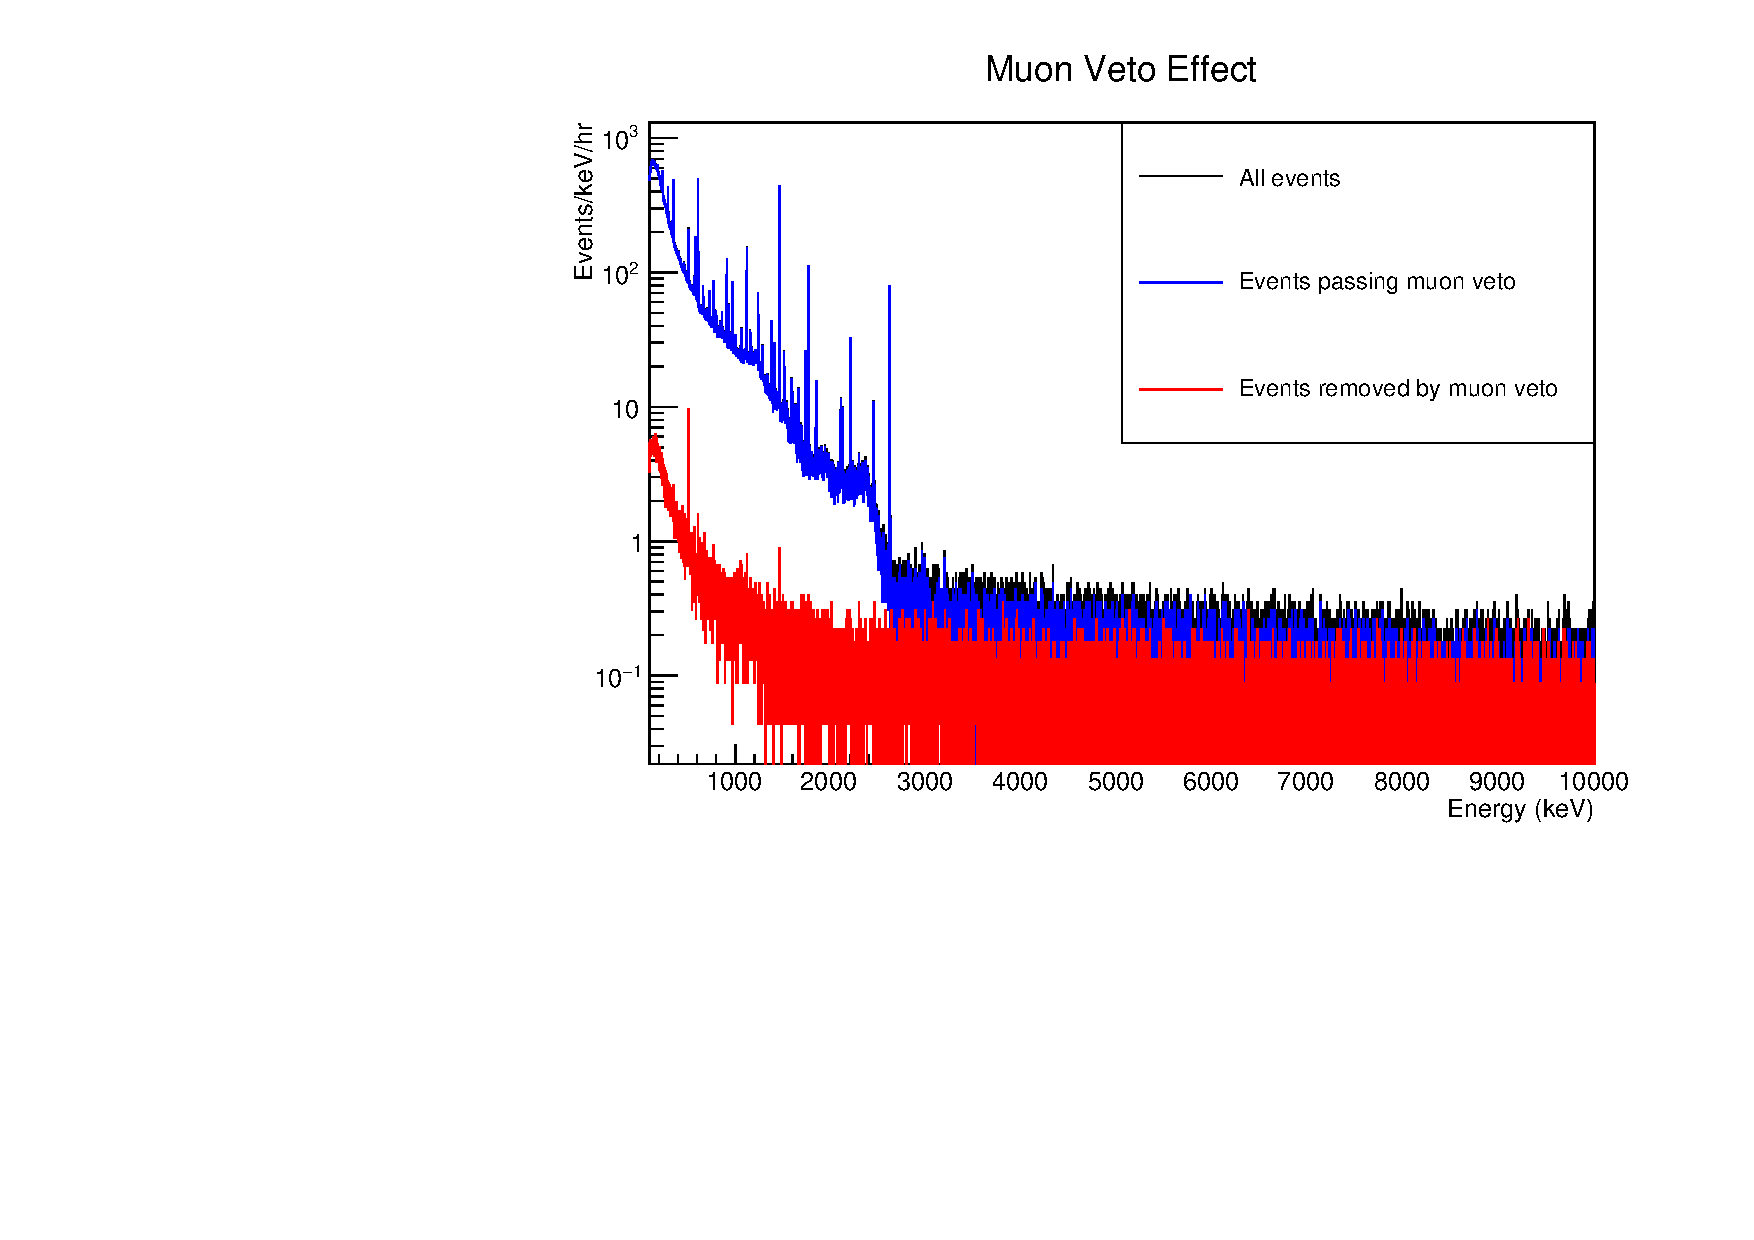
\includegraphics[height=3in]{/Users/jgruszko/Documents/Thesis/Plots/Ch5/muon_veto}
 \caption[The TUBE Ge energy spectrum, before and after the muon veto is applied]{The Ge energy spectrum, before and after the muon veto is applied (in black and blue, respectively), and the Ge spectrum of vetoed events (in red). Note that the largest peak in the veto spectrum is seen at 511\,keV, as is expected from true coincidence events due to pair production in materials near the detector, with a second small peak appearing at 1022\,keV. An additional small peak is seen at 1460\,keV, due to the high random coincidence rate of $^{40}$K events, likely from the PMT itself.}
 \label{fig:muVeto}
\end{figure}

\subsubsection{Live Time Analysis}
The dead time contributions of the Ge detector and veto system should be similar. The Ge detector triggers at approximately 60\,Hz, with a trigger window of 30\,$\mu$s and the muon veto system triggers at approximately 90\,Hz with a trigger window of 20\,$\mu$s. Each system contributes an expected dead time fraction of 0.18\%, leaving a total expected live time fraction of 99.64\,\%. 

In the the average data set used in this analysis, which is 22 hours long, the live time reduction gives 0.08\,hours (or less than 5 minutes) of dead time. 

Given the smallness of this effect compared to the statistical uncertainties in this analysis, the second-order effect of accidental coincidences is negligible, and is neglected.  

\subsection{Alpha Event Rate}\label{ssec:rate}
As a result of the as-built misalignment of the scanning and fixed IR shield axes (see Sec.~\ref{ssec:geometry}), the alpha event rate varies with scanning position. Since the degree of misalignment is not known {\it a priori}, it is estimated from the data. The fits to the energy spectra described in Sec.~\ref{ssec:E_obs} are used to find the mean energy and width of the alpha peak, and a count of the Poisson excess above the alpha-source-free runs in a 5$\sigma$ window around the peak energy is used to estimate the rate at each position. The assumption of a gaussian shaped peak in the energy spectrum is a poor one at low-magnitude scanning radii (as discussed in Sec.~\ref{ssec:E_obs}), but the rate may be estimated at larger radii on either side of these near-point contact positions, where the gaussian assumption is a good one. These results may then be extrapolated to find the rate at the remaining positions. 

As seen in Fig.~\ref{fig:alpha_rate}, the source beam is not measurably obstructed between radii of -15\,mm and 30\,mm, and falls approximately linearly at larger-magnitude negative radii. This observation, and the total reduction in rate at the largest magnitude radii lead us to derive a misalignment of less than 2$\degree$. The horizontal misalignment must be less than 1\,mm, since no scanning positions have a completely obstructed source beam. The exact values cannot be derived, since they are degenerate with one another. 

\begin{figure}[]
 \centering
 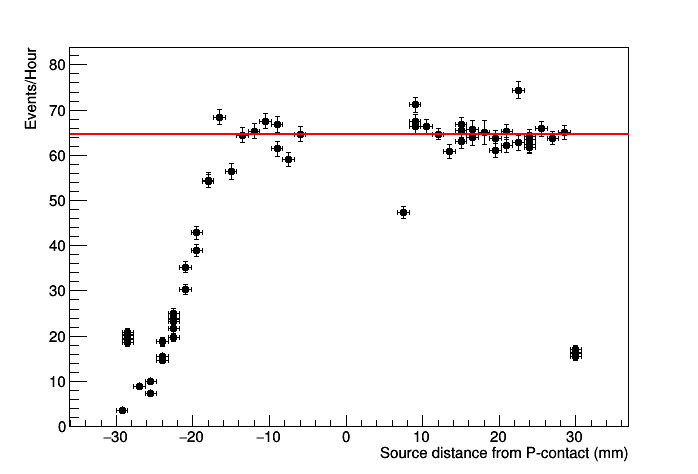
\includegraphics[width=1.0\columnwidth]{/Users/jgruszko/Documents/Thesis/Plots/Ch5/alphaRates_allPos_wAvg.png}
 \caption[Observed alpha event rates in each TUBE data set, following background subtraction]{Observed alpha event rates in each data set, following background subtraction. The red line indicates the average value, calculated as described in Sec.~\ref{ssec:rate}. The rate is reduced at positions with $r<-15$\,mm because of the misalignment of the scanning and IR cup axes. The rate at $r=7.5$\,mm is reduced by the partial obstruction of the passivated surface by the contact-pin holder, and the rate at $r=30$\,mm is low because the source beam is partially incident on the bevel, which is insensitive to alphas.} 
 \label{fig:alpha_rate}
\end{figure}

Scanning radii between -15\,mm and 30\,mm are used to calculate the observed alpha source rate. The point at $r = 7.5$\,mm is not included, since the source beam is partially obstructed by the contact-pin support at this position. The points at $r = 30$\,mm are also not included, since at this position, part of the source beam falls on the bevel, rather than on the passivated surface. The bevel is part of the n+ contact of the detector, which is insensitive to alpha interactions. Using the remaining the 32 measurements, the observed source rate is 64.6$\pm$0.5\,events/hr, or 18\,mBq.

Given that the standard deviation of the alpha event peaks (see Table~\ref{tab:E_fit_results}) is larger than the 43\,keV energy difference between the two $^{241}$Am $\alpha$ decay peaks, nearly the full activity of the source is expected to appear in the peak. Therefore, the observed activity is in excellent agreement with that expected from the source specifications and collimator geometry. 

 
% ========== Chapter 6
 
\chapter {Characterizing Surface Alpha Interactions with the TUBE Scanner}\label{ch:TUBE_analysis}

\section{Alpha Energy and Spectral Shape}
\subsection{Observations}\label{ssec:E_obs}
In the energy spectra for each data set, it can be seen that for large-magnitude radii, compared to source-free runs, there is an excess of events falling in a Gaussian peak, as in the examples in Fig~\ref{fig:Epeaks}. The energy and width of the peak varies with radius. For positions with radii larger than 6.75\,mm in magnitude, the mean alpha energy is larger than 2614\,keV, limiting the gamma-interaction background contribution in the peak region. See Figs.~\ref{fig:Efit_110} and~\ref{fig:Efit_360} for several examples. Therefore, despite the low alpha interaction rate, the peak can be clearly identified and fit.

A tail of events at low energy is expected to occur along with the peak, due to variation in the alpha penetration depth. However, in practice, adding an exponentially modified Gaussian component to the peak fitting function does not improve the goodness of fit. The low alpha rate and large standard deviation of the Gaussian peak often lead the preferred fit of the tail function to accommodate the background, rather than improving the fit to the peak. 

In the fit, the background is modeled by a linear function, which accounts for the gamma pile-up and muon background remaining after muon veto, single-site, and pile-up cuts. No other event cuts are used to produce these spectra. The results of these fits are shown in Figs~\ref{fig:Efit_mu} and ~\ref{fig:Efit_sig}.

\begin{figure*}[]
 \centering
  \begin{subfigure}[t]{.45\textwidth}
 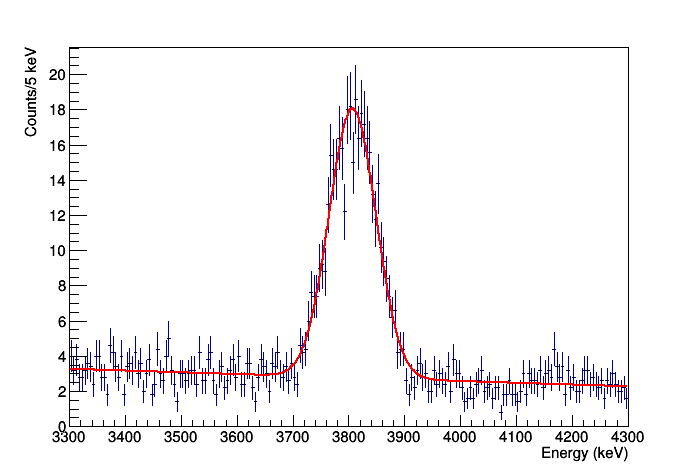
\includegraphics[width=1.0\columnwidth]{/Users/jgruszko/Documents/Thesis/Plots/Ch6/DS110_0_Efit.png}
  \caption{The energy spectrum of a data set taken at 11 turns ($r= -13.5$\,mm), a total of 25.1\,hrs of runtime.}
 \label{fig:Efit_110}
\end{subfigure}
\hfill
  \begin{subfigure}[t]{.45\textwidth}
 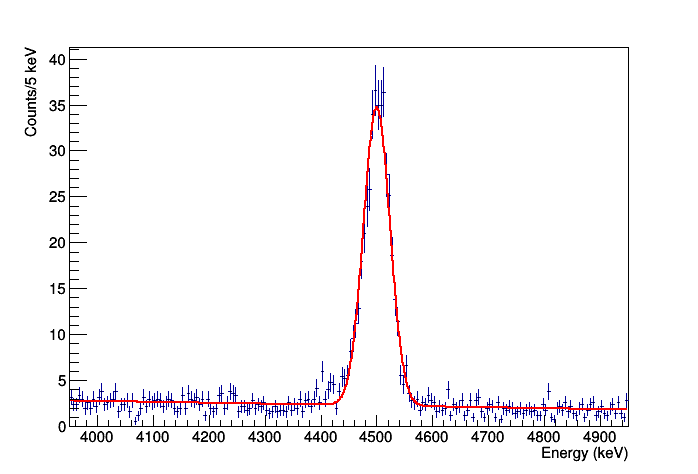
\includegraphics[width=1.0\columnwidth]{/Users/jgruszko/Documents/Thesis/Plots/Ch6/DS360_2_Efit.png}
  \caption{The energy spectrum of a data set taken at 36 turns ($r = 24$\,mm), with 30.1\,hrs of runtime.}
 \label{fig:Efit_360}
\end{subfigure}
\hfill
 \begin{subfigure}[t]{.45\textwidth}
 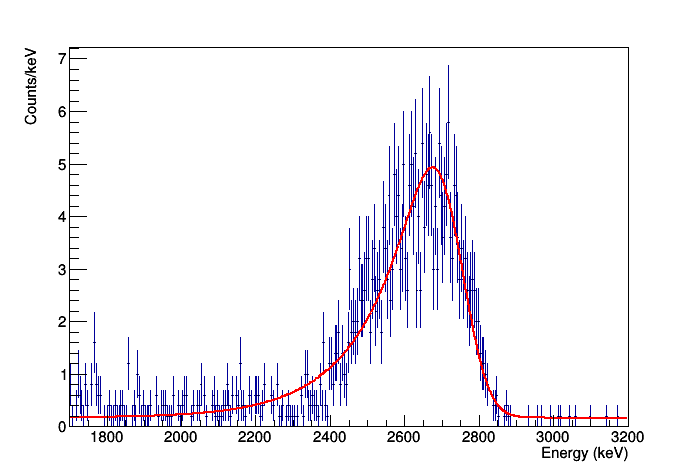
\includegraphics[width=1.0\columnwidth]{/Users/jgruszko/Documents/Thesis/Plots/Ch6/DS170_0_Efit.png}
  \caption{The energy spectrum of a data set taken at 17 turns ($r = -4.5$\,mm), a total of 19.1\,hrs of runtime, with a cut selecting near-point-contact events (${\tt aenorm} > 1.5$). At small radii ($r<6$\,mm), the peaks become highly non-Gaussian, and the fit is dominated by the low-energy tail. In addition to the fit results in Table~\ref{tab:Efits_aecut}, energy ranges for these small-radius positions are given in Table~\ref{tab:E_ranges}.}
 \label{fig:Efit_170}
\end{subfigure}
\hfill
 \begin{subfigure}[t]{.45\textwidth}
 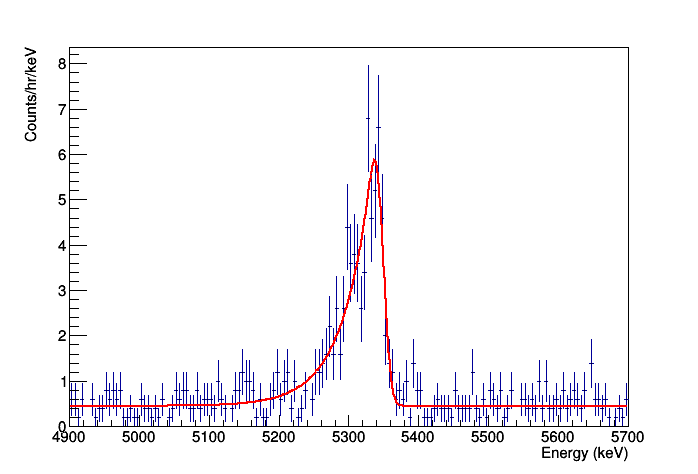
\includegraphics[width=1.0\columnwidth]{/Users/jgruszko/Documents/Thesis/Plots/Ch6/DS195_all_hiEfit.png}
 \caption{The sum energy spectrum of all runs taken at 19.5 turns ($r = -0.75$\,mm), a total of 82.4\,hrs of runtime, with a cut selecting near-point-contact events (${\tt aenorm} > 1.5$). Alphas incident on the point-contact have nearly the full incident energy, a narrower peak width, and visible low-energy tailing due to charge loss in the dead layer of the point-contact. Fit results are given in Table~\ref{tab:fullE_fitRes}.}
 \label{fig:Efit_195}
\end{subfigure}
 \caption{The energy spectra and peak fits for various scanning positions.} 
 \label{fig:Epeaks}
\end{figure*}

At radii smaller than 6\,mm, the alpha peak falls in a region of high gamma backgrounds. Due to the low alpha rate, it can not be fit without applying a pulse-shape cut to select the source events. A cut of ${\tt aenorm} >1.5$ selects near-point contact events while rejecting 99.8\% of background events. When this cut is applied, the remaining peak is highly non-Gaussian, as in Fig.~\ref{fig:Efit_170}. In these peaks, there is significant low-energy tailing, and the exponentially-modified Gaussian is included in the fit. The results of the fits are given in Table~\ref{tab:Efits_aecut}, where $\frac{1}{\tau}$ is the relaxation length (in keV) and  f$_{\tau}$ is the fractional contribution of the low-energy tail component to the peak area.

%\input{Efits.txt}

\begin{table*}[]
\begin{center}
\begin{tabular}{l l r r r r r}
Data Set & $\alpha$ Pos. (mm) & $\mu$ (keV) & $\sigma$ (keV) & f$_{\tau}$ & $\tau$ (keV$^{-1}$)& $\chi^2/N_{df}$ \\  \hline
{\tt DS170} & -4.5 & 2741$\pm$39 & 59$\pm$6 & 1.0$\pm$0.7 & 147$\pm$15 & 453/294 \\
{\tt DS180} & -3.0 & 2436$\pm$9 & 56$\pm$7 & 1.00$\pm$0.01 & 607$\pm$43 & 282/264 \\
\end{tabular}
\caption[The results of fits to the alpha energy peak at low-magnitude scanning radii]{The results of a Gaussian+low energy tail peak shape fit to the energy of alphas incident at small radii. A cut selecting near-point-contact events (${\tt aenorm} > 1.5$) is used to reduce the gamma background rate.} \label{tab:Efits_aecut}
\end{center}
\end{table*}

Due to the significant low-energy tail at these small radii, the Gaussian peak width does not give an accurate energy range for the alpha events observed. For the smallest radii ($r<3$\,mm), the Gaussian+tail model fit fails completely. For these data sets, we have given the estimated energy range of the observed alpha events, in Table ~\ref{tab:E_ranges}, either in lieu of or to supplement the description of the alpha energy spectra given by the fit results. These ranges were determined by eye-- they are the upper and lower energy bounds of the contiguous overdense region of high-A/E events that appear in the alpha-source runs, as in the boxed region of Fig.~\ref{fig:AEvE}.

\begin{table}[]
\begin{center}
\begin{tabular}{l l r r}
Data Set& $\alpha$ Pos. (mm) & $E_{min}$ (keV) & $E_{max}$ (keV) \\  \hline
{\tt DS170} & -4.5 & 2300 & 2850 \\
{\tt DS180} & -3.0 & 1200 & 2600 \\
{\tt DS185} & -2.25 & 700 & 2600 \\
{\tt DS190} & -1.5 & 800 & 2800 \\
\end{tabular}
\caption[Estimated energy ranges of alpha interactions at small-magnitude radii]{Estimated energy range of alpha interactions for source scans at small radii. At these positions, the peak is highly non-Gaussian. All data sets taken at each position are combined to determine these results.} \label{tab:E_ranges}
\end{center}
\end{table}

\begin{figure*}[]
 \centering
 \begin{subfigure}[]{.45\textwidth}
 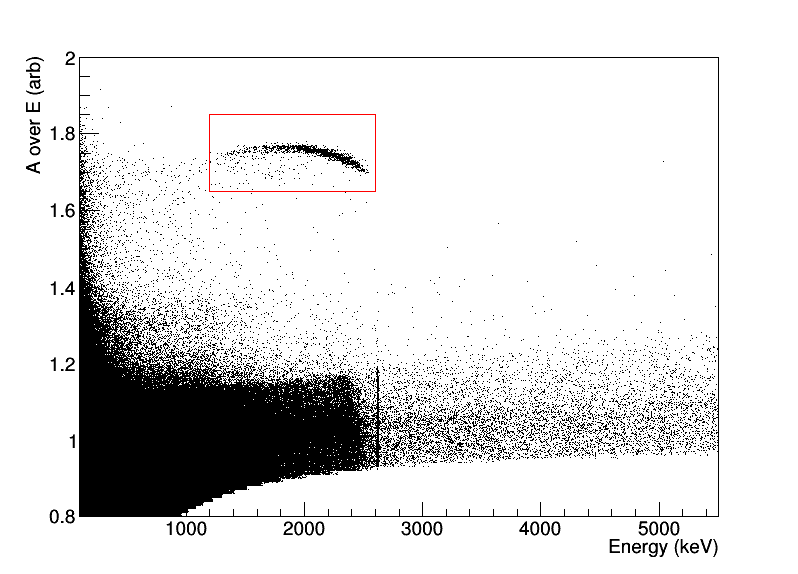
\includegraphics[width=1.0\columnwidth]{/Users/jgruszko/Documents/Thesis/Plots/Ch6/DS180_AE_all_wBox.png}
\end{subfigure}
 \begin{subfigure}[]{.45\textwidth}
 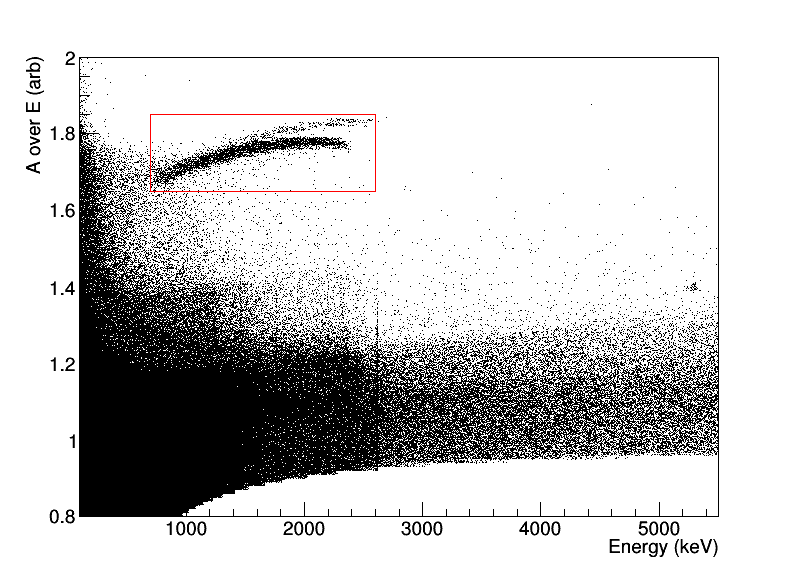
\includegraphics[width=1.0\columnwidth]{/Users/jgruszko/Documents/Thesis/Plots/Ch6/DS185_AE_all_wBox.png}
\end{subfigure}
 \caption[Plots of A/E vs. E for small-magnitude radii scans.]{At small radii, ({\it left:} $r=-3.0$\,mm, {\it right:} $r=-2.25$\,mm) the alpha peak becomes highly non-Gaussian and becomes impossible to fit with a Gaussian+low energy tail model. Depending on the scanning position, the energy ranges of the high-A/E alpha events (indicated by the boxed regions above and listed in Table~\ref{tab:E_ranges}) are given to supplement or stand in place of the fit result information.} 
 \label{fig:AEvE}
\end{figure*}

At scanning positions that are partially or entirely incident on the point-contact, an additional alpha peak in the spectrum appears at nearly the full energy of the emitted alpha. Again, an A/E cut selecting near-point-contact events ($A/E>1.5$) is applied to reduce the muon background. The peak shape is well-approximated by the sum of a Gaussian and an exponentially-modified Gaussian, as is expected from energy loss in the point-contact itself. See Fig~\ref{fig:Efit_195}. The results of these fits are given in Table~\ref{tab:fullE_fitRes}, . In {\tt DS195}, the source beam is entirely incident upon the point-contact, instead of being partially incident on the passivated surface. In this data set, the mean of the Gaussian component of the alpha peak falls at 5345\,keV, 141\,keV below the full 5.486\,MeV alpha energy. 

All of the peak energies of the fits to the alpha energy spectra are depicted in Fig.~\ref{fig:Efit_mu}, and the standard deviations of the gaussian components are depicted in Fig.~\ref{fig:Efit_sig}. Plotting these results as a function of the magnitude of the radius, as in Fig.~\ref{fig:Efit_rMag}, the results at the positive- and negative-radii scanning positions appear to be consistent. 

\begin{figure*}[]
 \centering
  \begin{subfigure}[]{\textwidth}
  \centering
 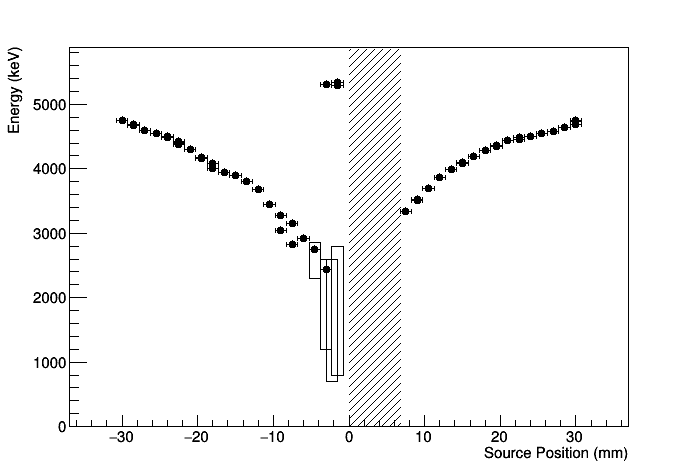
\includegraphics[height=3in]{/Users/jgruszko/Documents/Thesis/Plots/Ch6/EvR_wBoxes.png}
 \caption[The centroids of the alpha energy peaks in each data set]{The centroids of the alpha energy peaks in each data set. For scanning positions with significant low-energy tailing, the black box depicts the estimated full energy range of alpha events, as given in Table~\ref{tab:E_ranges}. At positions that are partially or completely incident on the point-contact, an additional peak appears at nearly the full incident alpha energy. } 
 \label{fig:Efit_mu}
\end{subfigure}
~
\begin{subfigure}[]{\textwidth}
\centering
 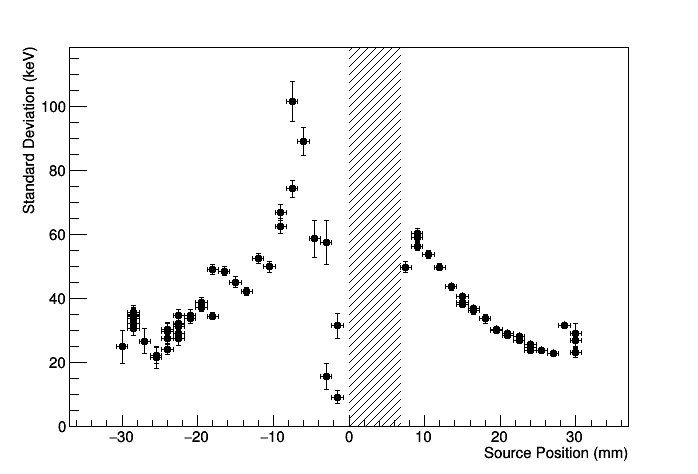
\includegraphics[height=3in]{/Users/jgruszko/Documents/Thesis/Plots/Ch6/EsigvR_wBoxes.png}
 \caption{The standard deviation of the gaussian component of the alpha energy peaks in each data set.} 
 \label{fig:Efit_sig}
 \end{subfigure}
 \caption[The results of Gaussian fits to the alpha energy peaks]{The results of Gaussian fits to the alpha energy peaks. The hashed box indicates the region on the detector surface that is obscured by the contact pin and contact pin support.}
\end{figure*}

\begin{figure*}[]
 \centering
 \begin{subfigure}[]{\textwidth}
 \centering
 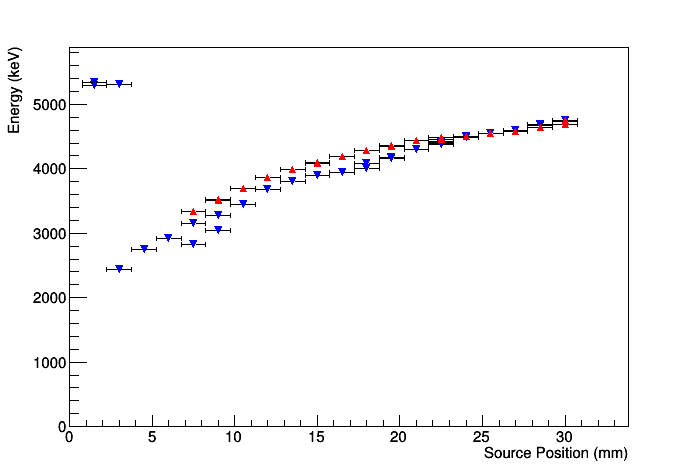
\includegraphics[height=3in]{/Users/jgruszko/Documents/Thesis/Plots/Ch6/EvRmag.png}
\end{subfigure}
 \begin{subfigure}[]{\textwidth}
 \centering
 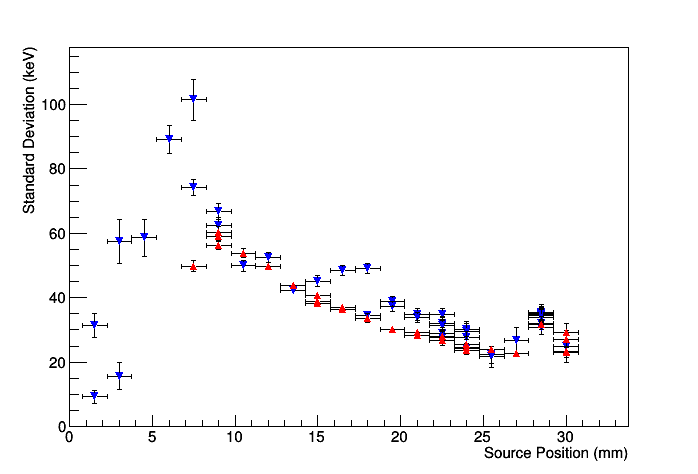
\includegraphics[height=3in]{/Users/jgruszko/Documents/Thesis/Plots/Ch6/EsigvRmag.png}
\end{subfigure}
 \caption[Energy fit results as a function of distance from the point contact]{The centroids {\it (top)} and standard deviations {\it (bottom)} of the alpha energy peaks in each data set, given as a function of the radial distract from the point contact. Negative-radius source positions appear as blue downward-pointing triangles, and positive-radius positions as red upward-pointing triangles. The results of the 0$\degree$ and 180$\degree$ scans appear to be consistent.} 
 \label{fig:Efit_rMag}
\end{figure*}

\begin{table*}[]
\begin{center}
\begin{tabular}{l l r r r r r}
Data Set & $\alpha$ Pos. (mm) & $\mu$ (keV) & $\sigma$ (keV) & f$_{\tau}$ & $\tau$ (keV$^{-1}$)& $\chi^2/N_{df}$ \\  \hline
{\tt DS185} & -2.25 & 5303$\pm$8 & 16$\pm$4 & 1.0$\pm$.9 & 12$\pm$11 & 314/274 \\
{\tt DS190} & -1.5 & 5298$\pm$5 & 31$\pm$4 & 0.3$\pm$.2 & 31$\pm$4 & 332/274 \\
{\tt DS195} & -0.75 & 5345$\pm$4 & 9$\pm$2 & 0.9$\pm$.1 & 41$\pm$6 & 335/274 \\
\end{tabular}
\caption[The results of fits to the alpha energy peak for events occurring in the point contact]{The results of a Gaussian+low energy tail peak shape fit to the energy of alphas incident on the point-contact. All data sets taken at each position are combined to determine these results.} \label{tab:fullE_fitRes}
\end{center}
\end{table*}

\subsection{Radial Dependence of Energy}\label{sssec:spec_fit}
Using the mean energies at each position found in Sec.~\ref{ssec:E_obs}, a spectral model describing the energy contributions of alpha contamination at a given position on the passivated surface can be constructed. Though it is slightly unnatural to consider the radial dependence of the energy, rather than the inverse, it will simplify the derivation of a full alpha energy spectrum for a given radial contamination model. Therefore we proceed with the former.

\begin{figure}[]
 \centering
 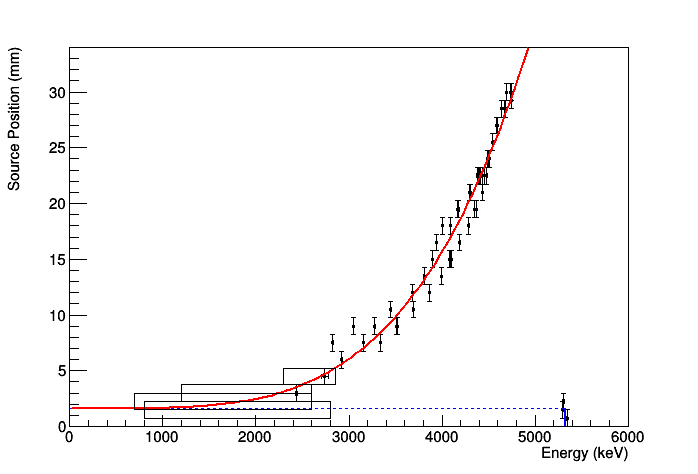
\includegraphics[width=1.\columnwidth]{/Users/jgruszko/Documents/Thesis/Plots/Ch6/RvsE_fit_wBoxes.png}
 \caption[A polynomial fit describing the radial dependence on energy]{Radii of the source incidence position, plotted with respect to the energy of the resulting alpha peak. Only data sets for which a gaussian (or gaussian+low-energy tail) peak shape modeled the alpha peak are included in the fit. The boxes represent the range of energies for the data sets that could not be fit, given in Table~\ref{tab:E_ranges}. The passivated-surface radii (scans with $r\geq3$\,mm), are fit with a fourth-order polynomial in energy (in red), and the energies of the point-contact positions are averaged (in blue).} 
 \label{fig:RvsE_fit}
\end{figure}

Plotting the radii of the measurements in which the source was incident on the passivated surface with respect to the centroid energies found at those radii, as in Fig.~\ref{fig:RvsE_fit}, and fitting to the fourth-order polynomial
$$ r = aE^4 + 1.6 $$
where $r$ is the source position radius, in mm, and $E$ is the energy of the resulting event, we find that the fit parameter $a = 5.50E-14\pm3E-16$, and the $\chi^2/N_{df}$ of the fit is 2.50.

The constant component is set to be 1.6\,mm because this is the outer radius of the point-contact of PONaMa-1; the passivated surface energy function should not exhibit a radial dependence below this value. When the constant component is allowed to float in the fit, it fits to a value of $1.4\pm.2$\,mm, consistent with a radius of 1.6\,mm. Therefore, we fix this parameter to the model-driven value. 

The choice of a fourth order polynomial was entirely driven by the observed spectral shape, and is not driven by any theoretical model. The goodness-of-fit is not improved by the addition of a quadratic component to the fitting function. If the polynomial of the fit is allowed to float, it fits to a value of $4.2\pm0.1$, and the $\chi^2/N_{df}$ of the fit is 2.44, only slightly improved from its previous value. Therefore, for the sake of simplicity, we fix the exponent to a value of 4.  

Though the energy spans of events at the lowest scanning radii (where a peak could not be fit to the spectrum) were not included in the fit, their range of values roughly agrees with those given by the fitting function. The increase in the width of the energy peak at low radii found from the derived spectral shape is not as dramatic as that seen in the data; if they matched, the red fit line in Fig.~\ref{fig:RvsE_fit} would traverse the full length (in the energy-axis) of each box. This, and the imperfect goodness-of-fit, indicates that there is additional energy-broadening that is not captured by the derived spectral shape function. However, this simple function appropriately captures most of the relevant energy information. 

To model the energies of alpha events on the point contact itself (at $r<1.6$\,mm), the mean energies of the 3 fits to the point-contact alpha peaks are averaged. Their average energy is $5323\pm3$\,keV. The energy at these radii is assumed to be independent of radius. 

\subsection{Discussion}
The energy of alpha events from the collimated source incident on the passivated surface of the detector is degraded at all radii, and is reduced far beyond the expected energy loss to a thin dead layer. Furthermore, the energy varies by up to a factor of 5 with the incident radius of the source. 

Both of these observations indicate that charge loss, whether to slow surface charge collection, charge trapping, or a combination of the two factors, is occurring. Additionally, the radial dependence of energy indicates that positive and negative charge carrier contributions are affected differently, as would be expected from their differing mobilities in germanium.

At positions near the point-contact of the detector, the relative contributions of electrons and electron-holes vary drastically over small distances. For instance, at radii less than 5\,mm, the weighting potential at the passivated surface of a detector similar to PONaMA-1 (see Fig.~\ref{fig:wp_z0}) varies by over 15\% over the diameter of the alpha source beam (1.75\,mm). At radii larger than 10\,mm, on the other hand, the weighting potential varies by less than 3\% over the diameter of the alpha source beam. 

Based on this difference in the weighting potential, the observed variation in the alpha source spectral peak shape is not unexpected. 

The weighting potential also allows us to infer that both positive and negative charges must be affected by the charge loss mechanism in the detector. If only the energy of the electrons were being lost, the alpha peak energy would be reduced by at most 10\% at radii larger than 13\,mm. Instead, we see, in Fig.~\ref{fig:Efit_mu}, the energy is reduced by up to 31\% of the full incident alpha energy for these radii. Overall, the energy dependence on radius is larger (steeper?) than the radial dependence of the weighting potential for all radii, with a difference that is particularly dramatic for large radii. 

If, instead, only the energy from the electron-holes were being affected, we would except the energy of the alpha peak to increase dramatically at radii less than 5\,mm. This is also not observed; the alpha peak falls steeply until the source beam is incident on the point contact itself, with peak energies below 50\% of the full alpha energy. 

Therefore, we must conclude that both positive and negative charges are being trapped and/or slowed for interactions near the passivated surface, regardless of the radial position of the interaction. Conclusions concerning possible charge-loss mechanisms are discussed in Sec.~\ref{sec:models}.

Events incident on the p-contact, on the other hand, do not show indications of significant charge-trapping. The average energy loss observed is consistent with the loss seen in scans of the point contact of BEGe-type PPC detectors \cite{Agostini_thesis}. In that work, the energy loss was found to indicate a dead layer thickness of $519\pm15$\,nm, larger than the manufacturer-cited Boron implantation depth of approximately 300\,nm. This could indicate the presence of additional material on the surface of the point-contact or deadness extending beyond the cited boron-implantation depth. 

\begin{figure}[]
 \centering
 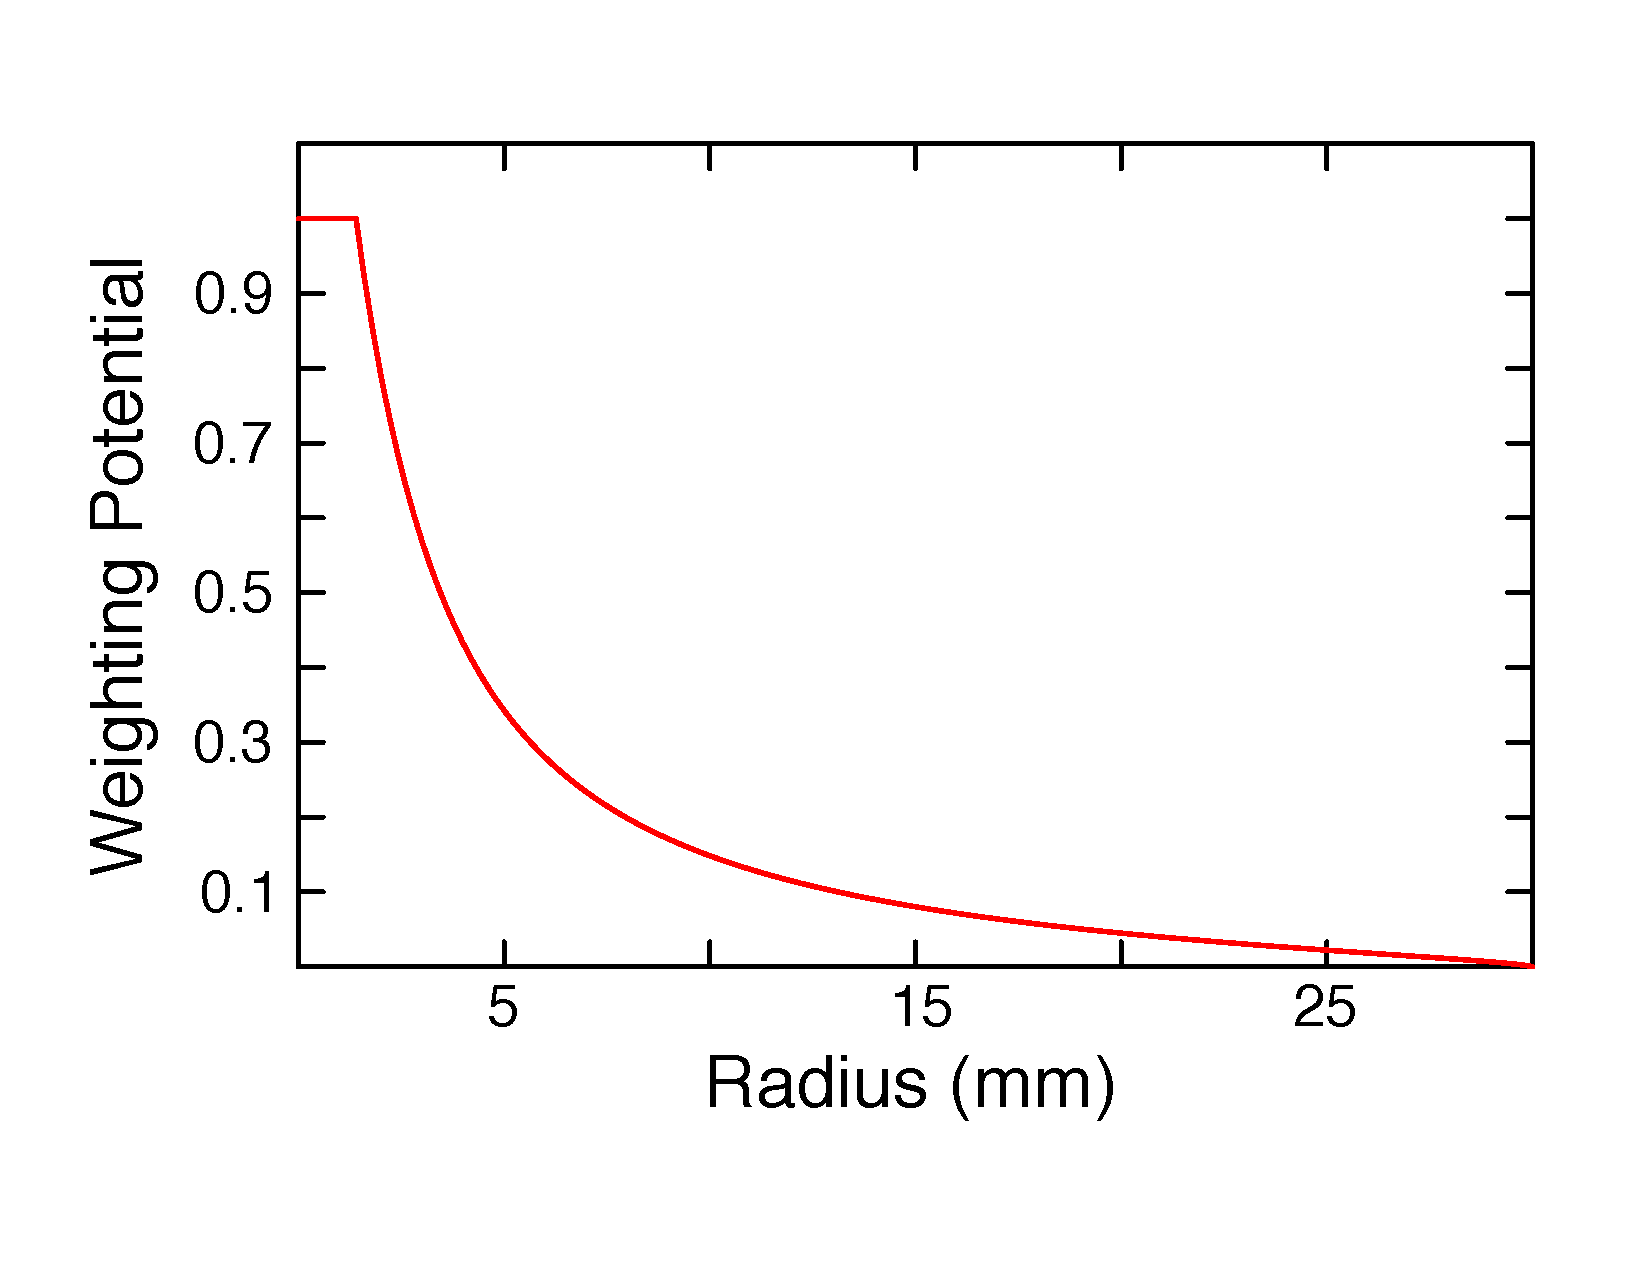
\includegraphics[height=3in]{/Users/jgruszko/Documents/Thesis/Plots/Ch6/wp_z0}
 \caption{The electron weighting potential at the passivated surface of a PPC detector similar to PONaMA-1. Calculated using {\tt fieldgen}.} 
 \label{fig:wp_z0}
\end{figure}

\section{DCR Parameter Values and Peak Shape}
\subsection{Observations}
In the DCR distribution for each data set, almost all alpha events fall in a gaussian peak. Fits to the alpha peaks in the DCR distributions are done for three of the parameters, {\tt dcr90}, {\tt dcrpzc90}, and {\tt dcrpzc99norm}. Deriving the results for alternate acceptance levels of the first two simply require a shift of the results, with no rescaling. The final version is provided to correct for the effects of gain shifts or changes in the pole-zero decay constant of the signal pulses, but is sensitive to changes in the noise of the system. 

\begin{figure*}[]
 \centering
  \begin{subfigure}[t]{.45\textwidth}
 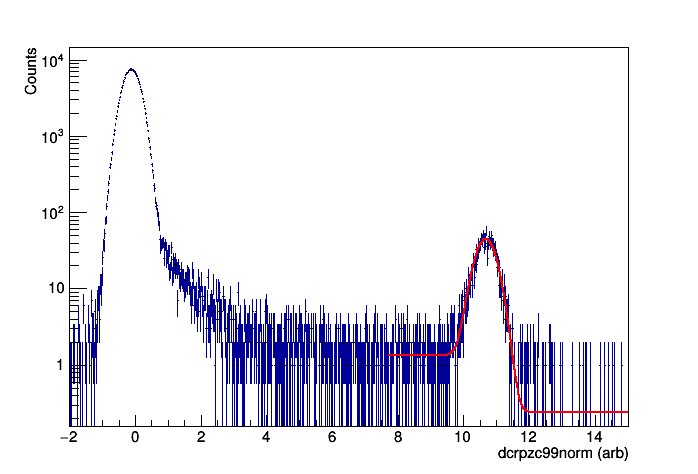
\includegraphics[width=1.0\columnwidth]{/Users/jgruszko/Documents/Thesis/Plots/Ch6/DS110_0_DCRPZCnorm.png}
  \caption{The {\tt dcrpzc99norm} distribution of a data set taken at 11 turns ($r= -13.5$\,mm), a total of 25.1\,hrs of runtime.}
 \label{fig:DCRfit_110}
\end{subfigure}
\hfill
  \begin{subfigure}[t]{.45\textwidth}
 \includegraphics[width=1.0\columnwidth]{/Users/jgruszko/Documents/Thesis/Plots/Ch6/DS360_2_DCRPZCnorm.png}
  \caption{The {\tt dcrpzc99norm} distribution of a data set taken at 36 turns ($r = 24$\,mm), with 30.1\,hrs of runtime.}
 \label{fig:DCRfit_360}
\end{subfigure}
\hfill
 \begin{subfigure}[t]{.45\textwidth}
 \includegraphics[width=1.0\columnwidth]{/Users/jgruszko/Documents/Thesis/Plots/Ch6/DS185_0_DCRPZCnorm.png}
  \caption{The {\tt dcrpzc99norm} distribution of a data set taken at 18.5 turns ($r = -2.25$\,mm), a total of 25.0\,hrs of runtime, with a cut selecting near-point-contact events (${\tt aenorm} > 1.5$). At small radii ($r<3$\,mm), the DCR parameter values for alpha events become similar to those of gamma background events.}
 \label{fig:DCRfit_185}
\end{subfigure}
\hfill
 \begin{subfigure}[t]{.45\textwidth}
 \includegraphics[width=1.0\columnwidth]{/Users/jgruszko/Documents/Thesis/Plots/Ch6/DS195_dcrpzcFit.png}
 \caption{The sum {\tt dcrpzc90} distribution of all runs taken at 19.5 turns ($ = -0.75$\,mm), a total of 82.4\,hrs of runtime, with a cut selecting near-point-contact events (${\tt aenorm} > 1.5$) in a $5\sigma$ energy window centered at the full-energy alpha peak position. Alphas incident on the point-contact do not show elevated DCR values.}
 \label{fig:DS195_dcrFit}
\end{subfigure}
 \caption[DCR parameter distributions and Gaussian fits for various peak positions]{DCR parameter distributions and Gaussian fits for various peak positions. The different varieties of DCR parameters generally have similarly-shaped distributions, save for peaks near 0 in {\tt dcrpzc99norm}, which are distorted by scaling effects. Fit results are given in Figs~\ref{fig:DCRfit} and \ref{fig:dcrNormFit}.} 
 \label{fig:DCRpeaks}
\end{figure*}

A full model-driven fitting function would include both a gaussian and exponentially-modified gaussian that accounts for the tail of low-DCR alpha events, seen in the plots of DCR vs. energy, in the fit to the peak. The background, which is the tail of the background-event gaussian, would be most appropriately modeled by a quadratic function. In practice, however, the fraction of alpha events occurring in the low-DCR tail small, and the relaxation constant of the tail is long. Combined with the low alpha rate, when a low-DCR tail is included, it is degenerate with the background function. Similarly, the inclusion of linear and quadratic components does not improve the fit to the background events. Instead, the combinations of the low-DCR tail of the signal and the low-DCR rise in the background can be fit effectively by including a step function (centered at the mean of the alpha peak gaussian) in the background function and limiting the fit window appropriately. Since the peak integral is not used for analysis, it is irrelevant whether the alpha peaks are fit with the signal or background components of the fit. 

The DCR spectrum includes all non-muon single-site events with energies between 1 and 6\,MeV. For $r > 3$\,mm, the energy of all observed alpha events falls in this range (see Table~\ref{tab:E_ranges}. Furthermore, the DCR value in the peak is sufficiently above the DCR distribution for normal events that the peaks can be clearly distinguished, and the high-DCR peak can be fit to a single Gaussian (see Figs~\ref{fig:DCRfit_110} and ~\ref{fig:DCRfit_360} for examples).

For data sets with $r<3\,mm$, the relevant energy range extends below 1\,MeV and the DCR values approach those of gamma background events, making the alpha event peak difficult to distinguish. As in the fits to the energy spectra, a pulse shape cut selecting near-point contact (${\tt aenorm} > 1.5$) events is applied to reduce the background rate and allow a fit to the alpha events (see Fig~\ref{fig:DCRfit_185}).

Events incident on the point contact itself do not have distinguishably distinct peaks in DCR when the broad energy range of 1 to 6\,MeV is used. Instead, the peak must be fit using an energy window in which the alpha events dominate the spectrum; a 5$\sigma$ window around the peak energy (taken from the fits described in Sec.~\ref{ssec:E_obs}) is used. Due to the low event and background rate after these cuts are applied, the peak is fit using only a Gaussian distribution. This approach is used only for the data sets with $r=-0.75$\,mm, the source position at which the beam is entirely incident on the point contact (see Fig~\ref{fig:DS195_dcrFit}).

All three of the DCR parameters are fit with the same procedure. The peak shapes in all three parameters are similar, save for at small radii ($r<6$\,mm), where the DCR parameter values are small and pole-zero corrected DCR parameters retain better alpha separation from the gamma and muon background events than the {\tt dcr90} value does. At very small DCR values, the {\tt dcrpzc99norm} peak shapes are distorted by the effects of the scaling on negative tail slope values. 

Results are given in Figs.~\ref{fig:DCRfit} and ~\ref{fig:dcrNormFit}. It is clear, both there and in the plots of the DCR values with respect to the magnitude of the radius (Figs.~\ref{fig:DCRfit_rMag} and ~\ref{fig:dcrNormFit_rMag}), that unlike the energy, the DCR parameter values of the alpha peaks do not appear to be azimuthally symmetric. At positions with $r>6$\,mm, the DCR values of alpha events are consistently much higher than those of background events; however, the value of the parameters differs by up to a factor of 2 at the $0\degree$ and $180\degree$ scanning positions. 

\begin{figure*}[]
 \centering
  \begin{subfigure}[t]{.45\textwidth}
 \includegraphics[width=1.0\columnwidth]{/Users/jgruszko/Documents/Thesis/Plots/Ch6/dcrCombined_mu.png}
 \caption{The centroids of the alpha peaks in each data set.} 
 \label{fig:DCRfit_mu}
\end{subfigure}
\hfill
\begin{subfigure}[t]{.45\textwidth}
 \includegraphics[width=1.0\columnwidth]{/Users/jgruszko/Documents/Thesis/Plots/Ch6/dcrCombined_sig.png}
 \caption{The standard deviation of the alpha peaks in each data set.} 
 \label{fig:DCRfit_sig}
 \end{subfigure}
 \caption[The results of Gaussian fits to the alpha peaks in {\tt dcrpzc90} and {\tt dcr90}]{The results of Gaussian fits to the alpha peaks in {\tt dcrpzc90}, in black, and {\tt dcr90}, in blue. All values are in units of ADC/ns. The hashed box indicates the region on the detector surface that is obscured by the contact pin and contact pin support.}
  \label{fig:DCRfit}
  
   \centering
  \begin{subfigure}[t]{.45\textwidth}
 \includegraphics[width=1.0\columnwidth]{/Users/jgruszko/Documents/Thesis/Plots/Ch6/dcrpzc99normfit_mu.png}
 \caption{The centroids of the alpha peaks in each data set.} 
 \label{fig:dcrNormfit_mu}
\end{subfigure}
\hfill
\begin{subfigure}[t]{.45\textwidth}
 \includegraphics[width=1.0\columnwidth]{/Users/jgruszko/Documents/Thesis/Plots/Ch6/dcrpzc99normfit_sig.png}
 \caption{The standard deviation of the alpha peaks in each data set.} 
 \label{fig:dcrNormfit_sig}
 \end{subfigure}
  \caption[The results of Gaussian fits to the alpha peaks in {\tt dcrpzc99norm}]{The results of Gaussian fits to the alpha peaks in {\tt dcrpzc99norm}, in arbitrary units. The hashed box indicates the region on the detector surface that is obscured by the contact pin and contact pin support.}
  \label{fig:dcrNormFit}
\end{figure*}

Additionally, the positive and negative radius positions show different qualitative behavior for $r>12$\,mm. At the negative-radius positions, the DCR parameters values rise as the radius increases, and at positive-radius positions, their values fall with increasing radius. 

At positions with $r<= 12$\,mm, the $0\degree$ and $180\degree$ scans are in greater agreement, though their values of {\tt dcr90} and {\tt dcrpzc90} are still offset from one another, as in Fig.~\ref{fig:DCRfit_rMag}. Correcting for changes in the gain and noise of the system, as in \ref{fig:dcrNormFit_rMag}, brings the values at these radii into closer agreement. In this plot, it can also be seen that the DCR's functional dependence on radius is in agreement for these near-point contact positions. 

A discussion of the potential causes of the observed azimuthal dependence, along with further discussion of the DCR parameter significance, is given below. 

\begin{figure*}[]
 \centering
 \begin{subfigure}[]{\textwidth}
 \centering
 \includegraphics[height=3in]{/Users/jgruszko/Documents/Thesis/Plots/Ch6/dcrCombined_mu_rMag.png}
\end{subfigure}
 \begin{subfigure}[]{\textwidth}
  \centering
 \includegraphics[height=3in]{/Users/jgruszko/Documents/Thesis/Plots/Ch6/dcrCombined_sig_rMag.png}
\end{subfigure}
 \caption[{\tt dcrpzc90} and {\tt dcr90} fit results as a function of distance from the point contact]{The centroids {\it (left)} and standard deviations {\it (right)} of the alpha DCR peaks in each data set, given as a function of the radial distract from the point contact. Both {\tt dcrpzc90} and {\tt dcr90} values are shown, in filled and open triangles, respectively. Error bars are suppressed for clarity. Negative-radius source positions appear as blue ({\tt dcrpzc90}) or green ({\tt dcr90}) downward-pointing triangles, and positive-radius positions as red ({\tt dcrpzc90}) or violet ({\tt dcr90}) upward-pointing triangles. The centroids of the 0$\degree$ and 180$\degree$ scans are not consistent with other another, but the peak widths appear relatively consistent. See~\ref{sssec:DCRfit_disc} for discussion.} 
 \label{fig:DCRfit_rMag}
\end{figure*}

\begin{figure*}[]
 \centering
 \begin{subfigure}[]{\textwidth}
 \centering
 \includegraphics[height=3in]{/Users/jgruszko/Documents/Thesis/Plots/Ch6/dcrpzc99normfit_mu_rMag.png}
\end{subfigure}
 \begin{subfigure}[]{\textwidth}
  \centering
 \includegraphics[height=3in]{/Users/jgruszko/Documents/Thesis/Plots/Ch6/dcrpzc99normfit_sig_rMag.png}
\end{subfigure}
 \caption[{\tt dcrpzc9norm} fit results as a function of distance from the point contact]{The centroids {\it (left)} and standard deviations {\it (right)} of the alpha {\tt dcrpzc99norm} peaks in each data set, given as a function of the radial distract from the point contact. The centroids of the 0$\degree$ and 180$\degree$ scans are not consistent with other another at $r>12$\,mm, but the peak widths appear relatively consistent. See~\ref{sssec:DCRfit_disc} for discussion.} 
 \label{fig:dcrNormFit_rMag}
\end{figure*}

\subsection{DCR as an Alpha Rejection Parameter}\label{sssec:DCRfit_disc}
At almost all scanning radii, alpha events incident on the passivated surface show significant slow charge components, and therefore highly elevated values of the DCR parameters. Therefore, the DCR pulse shape parameters provide a powerful tool by which external alpha events can be identified in PPC detectors. 

The amount of energy being collected as slow charge in the first 20\,$\mu$s of the pulse tail can be calculated directly from the {\tt dcrpzc90} parameter and the calibration constants for the electronics system. A {\tt dcrpzc90} value of 4E$-3$\,ADC/ns, similar to that found for many source positions, is divided by 0.74\,ADC/keV, the average value of the linear term of the energy calibration curve, to give an average rate of delated charge recovery in the pulse of 5.4\,keV/ns. The other terms of the calibration curve are relatively small, and are neglected. Therefore, in the 20\,$\mu$s of waveform tail that are digitized in these measurements, approximately 110\,keV of energy is collected. 

For each scanning position, we can find the slow component energy as a fraction of the prompt alpha peak energy at that position, as in Fig.~\ref{fig:Efrac}. The delayed charge energy fraction falls quickly at small scanning radii. At radii larger than 6\,mm, between 2.0 and 3.6\% of the total energy is collected as delayed charge, with an average delayed fraction of 2.5\%.  

\begin{figure}[]
 \centering
 \includegraphics[height=3in]{/Users/jgruszko/Documents/Thesis/Plots/Ch6/slowFracOverE.png}
 \caption{The energy of the collected delayed charge, as a fraction of the prompt alpha energy at that scanning position.} 
 \label{fig:Efrac}
\end{figure}

The alpha background events of interest to rare event searches like the \MJ\ \DEM\ are those with energies of over 1\,MeV. Given the typical PPC detector energy resolution of less than 5\,keV at these energies, a 2\% delayed charge effect, corresponding to 20\,keV, is easily observable. This implies that regardless of the source of the alpha background, and whether the alpha particle is degraded in energy before reaching the passivated surface, any event that has high enough energy to be a problematic background event also demonstrates a detectable delayed charge signature, provided its point of incidence is at at a radius greater than 6\,mm. 

\subsection{Outlier Events}\label{sssec:outliers}
When we plot a given alpha scan data set in the DCR vs. energy parameter space, as in Fig.~\ref{fig:outliers}, some fraction of outlier events that do not fall either in the alpha energy or DCR peak also appear. This implies that the Gaussian model of the peak position and shape (in both energy and DCR) does not fully describe all of the observed alpha events. Some events have both degraded energies and DCR values. 

Significantly for our purposes, the fraction of the prompt energy that is collected as slow charge (i.e. the ratio of {\tt dcrpzc90}, in keV/ns and integrated over the duration of the waveform tail, to the energy) in these events appears to be constant, and is 2.9\%, identical to that of the undegraded events. This means that, as discussed in Sec.~\ref{sssec:DCRfit_disc}, these events can still be efficiently identified in the \nonubb\ ROI.

The fraction of events that appear as outliers in both parameters is impossible to calculate precisely, since they become indistinguishable from the statistical fluctuation of background events at low energies and DCR values. Based on the numbers of events at higher-than-usual DCR values, we estimate that approx. 10\% of events are outliers. 

It is difficult to speak to the physics of these outlier events, since we do not know their origin. Though the source manufacturer cites a 20\,keV expected line-width for the $^{241}$Am source, that does not preclude the possibility of some small fraction of events being highly degraded in energy upon leaving the source. Another possibility is that these events are scattering in the collimator before arriving at the detector surface.

Alternatively, the degraded outlier events could be caused by a dead layer or shallow angle scattering in the passivated surface itself. Therefore, events such as these could be useful in understanding further aspects of charge collection from surface events, and in measuring the dead-layer associated with the passivated surface. 

Without knowing the origin of the outlier events, however, we cannot draw conclusions based on them. Future passivated-surface studies with the TUBE cryostat will employ source beams with shallower angles of incidence; based on the results of those studies, we should be able to determine the cause of these events and the thickness of the dead and charge-trapping regions associated with the passivated surface. 

\begin{figure}[]
 \centering
 \includegraphics[width=1.0\columnwidth]{/Users/jgruszko/Documents/Thesis/Plots/Ch6/outlier_events_260_0.png}
 \caption[DCR vs. energy in a data set, showing outlier events]{A plot of all single-site events in a data set taken at $r=9$\,mm, in {\tt dcrpzc90} vs. energy. The blue box shows the region that lies within $5\sigma$ of the energy and DCR peaks, and the red box indicates some of the events that are outliers from both peaks. Events that are in the violet box but not in the red or blue boxes are outliers in either the energy or DCR peaks. The red-outlined region shows a clear excess of events over a source-free data set. 8.2\% of the events in the violet box (including the red and blue-boxed regions) are outliers from both peaks; 89.2\% fall within the $5\sigma$ windows of both the energy and DCR peaks.} 
 \label{fig:outliers}
\end{figure}


\subsection{Radial Dependence of DCR}
The azimuthal dependence (or, we believe, the instability, see below) of the DCR parameters makes it difficult to draw definitive conclusions about their radial dependence. This is particularly the case at large radii ($r>12$\,mm). In positive-radius scanning positions, {\tt dcrpzc90} falls with increasing radius, at a rate of -4.8E-5$\pm$1.2E-5\,ADC/ns/mm, found using a linear fit to all data sets in this position range. In negative-radius scanning positions, {\tt dcrpzc90} instead rises with increasing radius, at a rate of 2.8E-5$\pm$3E-6\,ADC/ns/mm. 

Compared to this, the radial dependence of the DCR parameters at positions with $r<12$\,mm is dramatic, and occurs with similar functional form in both the positive- and negative-radius scans, as seen in Figs. ~\ref{fig:DCRfit_rMag} and ~\ref{fig:dcrNormFit_rMag}. Unfortunately, the source beam is obstructed at small positive-radii positions, so the similarity of the results cannot be tested directly for all radii. 

Over the range that can be scanned, though, the positive-radius positions show a fall {\tt dcrpzc90} rise with increasing radius with a rate of 1.4E-4$\pm$3E-5\,ADC/ns/mm, and the negative-radius positions show an increase with the rate of 3.2E-4$\pm$2E-5\,ADC/ns/mm. If, instead of using all negative-radius data sets, we use only those for which a positive-radius equivalent exists, we derive a rate of change for the {\tt dcrpzc90} value of 1.8E-4$\pm$4E-5\,ADC/ns/mm, which agrees with the rate found at positive-radius positions to within the uncertainty of the fit. 

Most importantly, we find that at incidence positions very close to the point-contact ($r<6$\,mm), the DCR parameters cannot be used to reliably identify alpha events while retaining high bulk-event efficiency. Alphas incident on the point-contact itself are completely indistinguishable by their DCR parameters.   

\subsection{Stability of the DCR Value}
The apparent azimuthal dependence of the DCR value is thought, rather, to be a problem of instability in the process by which delayed charge is collected. In studies of the stability, data sets with $|r|<12$\,mm are excluded; based on the observations of the radial dependence of DCR (above), it appears that the changes in DCR at these positions are unaffected by the azimuthal effect or instability, whatever its source. 

The leading candidate for the cause of the shift in the DCR parameters is charging of the detector surface by the alpha particles themselves, and the resulting interactions in the detector surface. Passivated surface charge build-up over time has been observed in other PPC detectors (citation?), and our own measurements of the observed energy indicate that significant charge is being lost on or near the surface. Direct measurement of the leakage current in the detector after the alpha scans were completed showed that it was an order of magnitude higher than at the start of scanning, further supporting this theory. 

\begin{figure}[]
 \centering
 \includegraphics[width=1.0\columnwidth]{/Users/jgruszko/Documents/Thesis/Plots/Ch6/dcrpzc90fit_mu_overTime_rOver12_wRate.png}
 \caption[DCR scan results as a function of data set order]{The {\tt dcrpzc90} mean value of the alpha peak, as a function of data set order. One data set corresponds, almost exactly, to one day of run time. The hashed boxes indicates stretches of time during which the alpha source was not incident on the detector surface. The color scale indicates the alpha event rate, in events/hr.} 
 \label{fig:DCRvT}
\end{figure}

Plotting {\tt dcrpzc90} in each data set with respect to the data set order (which corresponds, almost exactly, to days of run time), as in Fig.~\ref{fig:DCRvT}, shows a pattern in which the DCR parameter values rise over the time during which the source is incident on the passivated surface, ``resetting" to lower values after the source beam is removed from the surface for some time. Furthermore, the rate at which the DCR value increases appears to be correlated with the observed alpha rate, as would be expected if surface charge build-up were the cause of the change. 

Additional evidence for this theory is provided by the changes in DCR values in the positions that were repeated non-consecutively, with several days of scanning of other positions occurring between the two scans at that location. This was done for 3 positions, at $r= $  -9, -7.5, and 30\,mm. In all three cases, shown in Fig.~\ref{fig:DCR_repeated}, the second measurement shows a higher DCR value than the first measurement.  

\begin{figure}[t]
 \centering
 \includegraphics[height=3in]{/Users/jgruszko/Documents/Thesis/Plots/Ch6/dcrpzc90_repeatedDS.png}
 \caption[The change in DCR parameter values over time at repeated scan positions] {The {\tt dcrpzc90} mean value of the alpha peak as a function of data set order for the non-consecutively repeated measurements. The point shapes indicate the position of the source (circles, squares, and triangles correspond to runs with $r=$ -9, -7, and 30\,mm, respectively), and colors indicate the run order (blue is the first data set taken at that position, red is the second). One data set corresponds, almost exactly, to one day of run time. The hashed boxes indicates stretches of time during which the alpha source was not incident on the detector surface.} 
 \label{fig:DCR_repeated}
\end{figure}



\section{A/E and DCR: Complementary Pulse-Shape Discriminators} 
\subsection{A/E of Surface Alpha Events}
As expected from the calculated drift paths of PPC detectors, the rate of the initial rise of pulses strongly depends on the event incidence radius, particularly near the passivated surface. The high-A/E peak of events associated with the alpha source was fit using a Gaussian function, and its centroid $\mu_{AE}$ was taken as the characteristic A/E value of the scanning location. Since the precise peak shapes of the A/E distributions are not of interest for this work, we use a simplified fitting model, with only a Gaussian component to identify the peak centroid and width. 

For runs in which the energy of the $\alpha$ peak is well over 2630\,keV ($\abs{r} > 7.5$\,mm), only events with energies between 2630\,keV and 6\,MeV are included. For data sets with $\abs{r} < 7.5$\,mm, where all or some of the alpha peak may fall outside this energy window, events with energies between 1 and 6\,MeV are included. See Fig.~\ref{fig:AE_fits} for sample A/E distributions and fits. 

\begin{figure*}[]
 \centering
 \begin{subfigure}[t]{.45\textwidth}
 \includegraphics[width=1.0\columnwidth]{/Users/jgruszko/Documents/Thesis/Plots/Ch6/DS10_0_aefit.png}
 \caption{A data set taken at 1 turn ($r=-28.5$\,mm), a total of 24.9\,hrs of runtime, with a cut selecting events with energy between 2630\,keV and 6\,MeV.}
\end{subfigure}
\hfill
 \begin{subfigure}[t]{.45\textwidth}
 \includegraphics[width=1.0\columnwidth]{/Users/jgruszko/Documents/Thesis/Plots/Ch6/DS170_0_aefit.png}
  \caption{A data set taken at 17 turns ($r=-4.5$\,mm), a total of 19.1\,hrs of runtime, with a cut selecting events with energy between 1\,MeV and 6\,MeV.} 
\end{subfigure}
\caption[Sample A/E distributions and Gaussian peak fits to alpha events]{Sample A/E distributions and Gaussian peak fits to alpha events.}
 \label{fig:AE_fits}
\end{figure*}

For most data sets, the peak in A/E is approximately Gaussian in shape. As in the case of energy, the peak becomes non-Gaussian at small radii, where the length scale of significant changes to the drift time of charges becomes small compared to the diameter of the source beam. At these small radii, however, the A/E values are well above those of 99\% of background events. 

Anomalously low values of A/E occur for events incident on the point-contact itself. Though these events have very fast rising edges, they also have a substantial slow electron fraction, which reduces the A/E value. To correctly identify events like these from the shape of their rising edge, a rise-time parameter, measuring time over which the pulse rises from the start of the prompt signal to a given fraction of its total amplitude (for instance, 50\% of the maximum pulse height), would be more appropriate than the A/E parameter used in this analysis. The \MJ\ Collaboration plans to implement such a pulse-shape discriminator, in addition to the {\tt avse} parameter that is currently used to reject multi-site events.

\begin{figure}[t]
 \centering
 \includegraphics[height=3in]{/Users/jgruszko/Documents/Thesis/Plots/Ch6/AEvR_wBox.png}
 \caption[The results of fits to A/E in each data set]{The centroids of the alpha peaks in A/E in each data set. The relatively low value of A/E for data sets with $r=-0.75$\,mm occurs because the large (relatively slow) electron component of the signal reduces the A/E value for these events.} 
 \label{fig:AEfit_mu}
\end{figure}

The fit results are displayed in Fig.~\ref{fig:AEfit_mu}. These results indicate that the high-A/E cut applied to give energy and DCR fit results,  as in Sec.~\ref{ssec:E_obs}, is appropriate.


\subsection{Demonstrating Complementarity of High-A/E and DCR Cuts}
The distributions of alpha events incident at various radii in the A/E vs. DCR parameter space (see Fig.~\ref{fig:AEvDCR_events}) suggest that the two pulse-shape analyses are highly complementary. This suggests that by using both the A/E and DCR pulse shape discriminators, we should be able to achieve excellent alpha event discrimination with only minimal sacrifice of bulk events. 

\begin{figure*}[]
 \centering
 \begin{subfigure}{.65\textwidth}
 \includegraphics[width=1.\columnwidth]{/Users/jgruszko/Documents/Thesis/Plots/Ch6/AEvDCRPZCnorm.png}
 \end{subfigure}
 \begin{subfigure}{.34\textwidth}
  \includegraphics[width=1.\columnwidth]{/Users/jgruszko/Documents/Thesis/Plots/Ch6/AEvDCR_plot_legend.png}
   \end{subfigure}
 \caption[The A/E vs. normalized DCR distribution at various scanning radii]{The A/E vs. normalized DCR distribution for all single-site events with energies between 100\,keV and 10\,MeV, at various scanning radii. The points in black are from a data set without the alpha source incident on the detector surface, and the scan data sets are shown in rainbow order, with red representing the smallest-radius scan. 99\% of calibration events with energies between 1000 and 2630\,keV fall below an A/E value of 1, and 99\% of calibration events with energies between 1000 and 2380\,keV fall below a {\tt dcrpzc99norm} value of 1.} 
 \label{fig:AEvDCR_events}
\end{figure*}

Examining the fit results to the DCR and A/E peaks supports this conclusion. The $5\sigma$ windows around each alpha peak should include 99\% of the events, assuming normally distributed values; by using an equivalent normalization for the A/E and DCR values, we can compare them directly, as in Fig.~\ref{fig:AEandDCR}. The y-axis in this figure indicates the alpha events' separation from bulk events-- 99\% of bulk events fall below 1, whether the relevant discrimination parameter is A/E or DCR. Also indicated are the 99.9\% acceptance points in each parameter, which occur at different values for A/E and DCR, indicating that the DCR distribution is more heavily-tailed than the A/E distribution. 

\begin{figure*}[]
 \centering
 \includegraphics[width=1.\textwidth]{/Users/jgruszko/Documents/Thesis/Plots/Ch6/AEandDCR_noThree.png}
 \caption[A plot of A/E and DCR alpha peak positions, showing the complementarity of the pulse shape discriminators]{The $5\sigma$ window containing the A/E and DCR alpha peak positions at each position, normalized to 99\% bulk acceptance of both cuts. The red points and magenta boxes indicate the centroids and $\pm 2.5\sigma$ values of the peaks in {\tt dcrpzc99norm}, and the green points and blue boxes indicate the same in {\tt aenorm}. The red dotted line and cyan dotted-dashed line are the 99.9\% acceptance points in DCR and A/E, respectively. The black dashed line indicates the 99\% acceptance point in both parameters.} 
 \label{fig:AEandDCR}
\end{figure*}

For each position measured, we find that either or both of the DCR and A/E discriminator parameters are well above the 99.9\% acceptance line for that parameter. This indicates that by applying 99.9\% bulk-acceptance cuts in both parameters, we can effectively eliminate alpha events occurring anywhere on the passivated surface. Ergo, total alpha event rejection with only 0.2\% sacrifice of bulk events should be possible in PPC detectors.

Another advantage of this method of alpha removal is that it is equally effective at all energies of the alpha events, save for the requirement that the energy of the event be high enough that the DCR signal (of approximately 2-3\% of the prompt event energy, see above) is detectable. This is the case for all events that could fall in the \nonubb\ ROI. Therefore, this purely pulse-shape-based method is as effective for energy-degraded alpha events as it is for undegraded events originating from alpha contamination on the surface itself.

The only exception to this highly efficient alpha event removal occurs for events directly incident on the point-contact itself, at the smallest-radius position. Given that these events do not experience charge trapping, their energies are much higher than that of the \nonubb\ region-of-interest, so they are not a particularly problematic background. If alpha energy is degraded before reaching the point-contact, though, they could have any energy below the full energy of the alpha peak. As discussed above, these events would be effectively tagged with high efficiency if a rise-time parameter were substituted for the A/E parameter, as is planned in the \MJ\ \DEM\ analysis. 

Fig.~\ref{fig:AEandDCR} also shows that at positions with $r<= 6$\,mm, the A/E-based rejection of alpha events dominates in effectiveness, and that below $r=9$\,mm, an 99.9\%-acceptance cut in A/E suffices to tag all alpha events. This is why the previous study of alpha backgrounds in a PPC detector \cite{Agostini_thesis}, found no need for an additional pulse-shape discriminator beyond A/E, though an asymmetry parameter, which identifies slowly-released charge like our DCR parameter, was studied \cite{TUBEdoc?}. BEGe-type detectors, like the one measured in that work, have the entirety of their passivated surface lying within $r=9$\,mm, so the use of the DCR discriminator would not measurably improve their background rejection capabilities. 

The DCR discriminator is needed, though, in ORTEC-type detectors, which have a passivated surface along the entire bottom plane of the detector. In this detector design, which is that of the detector measured in this work, and used for all of the \MJ\ \DEM 's enriched detectors, the DCR discriminator is a powerful way to reject alpha events occurring far from the point-contact, where A/E is relatively insensitive. 

\subsection{Alpha-Identification Efficiency using DCR Techniques}
Given that the DCR pulse-shape discrimination technique is less effective than the A/E technique at $r<=6$\,mm, we focus our attention on evaluating the alpha-rejection efficiency of the various DCR parameters at scanning positions with $r>6$\,mm. 

To calculate an alpha-rejection fraction, we must first find the predicated number of background events in the alpha peak region of the data set, with no DCR cut applied. We use both the right-hand sideband in the data set and the spectral shape in the sideband and peak regions, measured in a source-free run, to find the expected number of background events. See Fig.~\ref{fig:eff_regions} for sample spectra and energy regions. 

\begin{figure*}[]
 \centering
 \includegraphics[width=1.\textwidth]{/Users/jgruszko/Documents/Thesis/Plots/Ch6/eff_peakRegions.png}
 \caption[Energy spectra, showing the windows used to calculate the DCR alpha rejection efficiency]{Energy spectra for a source scan data set with $r=9$\,mm {\it (left)} and a background data set {\it (right)}. The energy windows indicated are the $5\sigma$ peak region, in red, and the 500\,keV right-hand sideband, in blue. $n_{s, pk}$ is the sum of all events in the red solid-lined box and $n_{s, rh}$ is the sum of all the events in the blue solid-lined box. $n_{b, pk}$ and $n_{b, rh}$ are the sum of events in the red and blue dashed-line boxes, respectively.} 
 \label{fig:eff_regions}
\end{figure*}

Below, the background data set is referred to by the subscript {\it b} and the alpha source scanning data set by the subscript {\it s}. The peak region is taken to be a $5\sigma_E$ window around the centroid of the alpha-energy Gaussian, and the sideband region is the 500\,keV region with minimum energy of $\mu_E+5\sigma_E$. Only a right-hand sideband is used, to avoid effects from the energy-degraded alpha events described in Sec.~\ref{sssec:outliers}. The peak region is referred to by the subscript {\it pk}, and the sideband region by the subscript {\it rh}.

The following algorithm is repeated for each alpha scan data set for which we would like to calculate the efficiency:
\begin{itemize}
\item The expected spectral shape of the background events is calculated from a background run. To do this, the number of events in the peak region, $n_{b, pk}$, and the number of events in the right-hand sideband region, $n_{b, rh}$ are found. Each event total is divided by the width of its energy window. Their ratio is the number of events per keV expected in the peak region, given some number of events per keV in the sideband region.
\item The number of events in the right-hand sideband of the source scan data set, $n_{s, rh}$ is found. It is normalized by the width of the sideband energy window, and then multiplied by the width of the peak energy window and the spectral shape ratio to give the number of background events per hour expected in the peak region. 
\item This value is subtracted from the measured number of peak-region events in the alpha source scan data set, $n_{s, pk}$ to give the projected number of alpha events, $n_{\alpha}$. I.e., 
$$ n_{\alpha} =  n_{s, pk}-n_{s, rh}\frac{n_{b, pk}}{n_{b, rh}}\frac{5\sigma_E}{500\,keV} $$
\item The above steps are repeated after the DCR cut is applied to both the source and background runs to find the expected number of background events in the peak region of the source scan data set that would be removed by the cut. This value is subtracted from the total number of events cut in the peak region of the source data set to give the projected number of alpha events removed by the cut, $m_\alpha$. I.e.,
 $$ m_{\alpha} =  m_{s, pk}-m_{s, rh}\frac{m_{b, pk}}{m_{b, rh}}\frac{5\sigma_E}{500\,keV} $$
 where the $m_{i, j}$ are equivalent to the $n_{i, j}$ above, but measured after the DCR cut is applied. 
\item The ratio $\frac{m_\alpha}{n_\alpha}$ is the alpha rejection efficiency in the source-scan data set. 
\end{itemize}

A derivation of the formula by which the uncertainties for these efficiencies are calculated is given in Appendix FIXME. 

At positions with radii below 6\,mm for which the source is incident on the passivated surface, the alpha peak appears in a region of the energy spectrum that is dominated by gamma background events from environmental radioactivity and the materials of the cryostat itself. The alpha event rate is low, and these backgrounds are both high and highly variable. An additional complication comes from the broad energy distribution of the alpha events at these positions, as discussed in Sec.~\ref{ssec:E_obs}; to find an expected alpha event rate, we must understand the spectral shape over the entire range of relevant energies with high accuracy. 

This implies that our approach of normalizing the background spectra to one another is of limited utility.  The resulting uncertainties from the estimate of the backgrounds dominate our expected alpha event rate. Without an accurate calculation of the expected number of alpha events, we cannot accurately cite a rejection fraction for the events. Therefore, measurements at these radii are not included in the average efficiency values for each DCR parameter. 

Events incident on the point-contact itself are not expected to exhibit slow charge release, and are therefore expected to be relatively unaffected by the DCR cut. Data sets with the source beam incident on the point-contact are therefore also excluded from the average efficiency calculations. 

The rejection efficiencies are calculated for each data set using the {\tt dcr90}, {\tt mjddcr90}, and {\tt dcrpzc90}, and {\tt dcrpzc99norm} parameters. The first three of these are set to retain 90\% of single-site calibration events, and the final cut is set to retain 99\% of calibration events. The results for each data set are shown in Fig.~\ref{fig:eff_allR}, and the average rejection efficiency values for each parameter are given in Table~\ref{tab:avgEff}. 

The errors for the efficiency of each data set are large, due to the low alpha rate. They are particularly large at positions with large-magnitude negative radii, where the source beam is partially obscured. 

Averaging the efficiency at all scanning positions, however, reduces the error sufficiently to show that the rejection efficiencies of the various DCR parameters, save for {\tt dcrpzc99norm}, are consistent with 99\%. This implies that 1\% of alpha events with the full expected energy (indicating that significant charge trapping has occurred) are not measurably re-releasing that charge on the time scale of digitization. The higher average efficiency of the normalized DCR parameter ({\tt dcrpzc99norm}), which is consistent with 100\%, suggests that the culprit may be varying noise in the system, which is corrected for by the use of this parameter. This is unsurprising, given the high noise (and particularly the high and varying levels of microphonic noise, due to the vacuum pump operation) in the TUBE scanning setup. 

\begin{figure*}[]
 \centering
 \begin{subfigure}[]{\textwidth}
 \centering
 \includegraphics[height=3in]{/Users/jgruszko/Documents/Thesis/Plots/Ch6/dcrpzc_eff.png}
 \caption{The DCR parameters that employ event-by-event pole-zero correction. Values for {\tt dcrpzc90} are in red, and those for {\tt dcrpzc99norm} are in blue.} 
 \end{subfigure}
 \hfill
  \begin{subfigure}[]{\textwidth}
  \centering
 \includegraphics[height=3in]{/Users/jgruszko/Documents/Thesis/Plots/Ch6/dcr_eff.png}
 \caption{The DCR parameters that employ the linear projection method of pole-zero correction. Values for {\tt dcr90} are in red, and those for {\tt mjddcr90} are in blue.} 
 \end{subfigure}
 \caption[The alpha rejection efficiency as a function of radius for each DCR parameter]{The alpha rejection efficiency of each DCR parameter, calculated for each data set with a source beam incidence position with $r>6$\,mm.}
 \label{fig:eff_allR}
\end{figure*}

\begin{table}[]
\begin{center}
\begin{tabular}{l r r}
DCR Param. & ~~$\varepsilon$ (\%), $|r|>6$\,mm \\  \hline
{\tt dcr90} & 99.2$\pm$0.5  \\
{\tt dcrpzc90} & 98.9$\pm$0.5  \\
{\tt mjddcr90} & 99.1$\pm$0.5  \\
{\tt dcrpzc99norm} &  99.7$\pm$0.4 \\
\end{tabular}
\caption{Average alpha rejection efficiencies for all evaluated DCR parameters.} \label{tab:avgEff}
\end{center}
\end{table}

\section{Comparison to Models of Surface-Charge Collection}
\subsection{Surface Drift of Electrons}
The original theoretical model for the DCR effect posited that slow surface-drift of electrons was responsible for the slow charge component, with holes being collected normally through the bulk \cite{Neutrino16}. Charge transport models in germanium \cite{Mullowney2012} suggest that charge carrier mobilities are 10 to 100 times slower for surface transport than for bulk transport. Given the overall lower mobility of electrons, and the lower weighting potential they experience over much of the detector surface (as in Fig.~\ref{fig:wp_z0}), we would expect that electrons would be much more susceptible to surface transport than electron holes. 

This effect can be modeled using the {\tt fieldgen} and {\tt siggen} software packages by generating the fields in the detector with the addition of a small amount of charge deposited on the passivated surface. This creates drift paths that run perpendicular to the passivated surface in a narrow region near the surface. Events that occur in this skin depth, like alpha interactions, will have degraded energies and a DCR contribution (see Fig.~\ref{DCR_wf}). Electrons that reach the surface as assigned a slower drift speed, in this case a factor of 2\% of the bulk drift speed (check this with Susanne). 

The radial dependence of energy, in this case, mimics the inverse of the electron weighting potential exactly, since the fraction of the signal carried by the electrons is missing at all radii (see Fig.~\ref{fig:sim_EvR_e}). Because the electron component of the pulse shape (which is the origin of the DCR signal, in this case) increases in strength at small radii, we would expect that the DCR effect would  be particularly large at radii very near to the point-contact radius. In general, it would be expected to decrease with increasing radius, as in Fig.~\ref{fig:sim_DCRvR_e}. 

Given the observed radial dependence of energy and DCR, this model is not confirmed by the TUBE measurements. Though surface drift of electrons may be occurring, it is not the dominant effect observed. 

\subsection{Passivated-Surface Trapping of Holes}
An alternative model, in which the collection of the electron-holes is also impeded by the passivated surface layer effects, was developed. If there is a high concentration of bulk trapping centers in a thin layer near the passivated surface, as suggested by the direct measurements of trapping made in segmented germanium detectors ~\cite{Abt2017}, then some fraction of the electron-holes will be trapped in the bulk of the detector. Slow rerelease of these charges would lead to a DCR effect, in addition to the prompt signal from untrapped electron-holes. The rate of this rerelease would be temperature-dependent \cite{?}. Additionally, the electron fraction is completely or almost completely lost to trapping or slow surface transport in this model, which as in the surface-electron model, is likely given electrons' lower mobility. 

Again, we model the resulting radial dependence of energy and the DCR parameter using {\tt siggen}. The electron contribution to the signal is completely turned off (assigned a drift speed of 1E-4 of the bulk speed), and a given fraction of the electron holes is delayed by convolving their signal with an exponential function with a time constant of 10\,$\mu$s. 

If the hole trapping fraction is constant across the surface of the detector, the radial dependence of energy again mimics the shape of the inverse of the weighting potential (check this?), but a larger fraction of the incident energy is lost at all radii. The radial dependence of the DCR, on the other hand, exhibits the opposite behavior as in the surface-electron model, decreasing dramatically at small radii. The electron-hole contribution to the signal drops dramatically at small radii (as seen in the weighting potential, Fig~\ref{fig:wp_z0}); since the DCR effect in this case scales with that fraction, it also disappears at small radii. 

The energies observed in the TUBE scan of PONaMA-1, and the radial dependence of the DCR parameters at near-point-contact positions (where instability effects are reduced), support this model for the surface alpha charge collection. Further {\tt siggen} simulations should answer the question of whether a constant trapping fraction is sufficient to give the observed radial dependence of energy, or if a radial dependence of the charge trapping is needed to reproduce the effect observed in these measurements. (Add these if possible.)

\subsection{Surface Drift of Electrons and Holes}
A final possibility for the behavior of charges near the passivated surface of the detector is that both electrons and electron-holes are exhibiting surface drift. Since the holes would drift more quickly, they would therefore dominate the DCR. Thus, the radial dependence of energy and DCR would be identical to that predicted by the bulk-trapping model. Alpha source scans at varying detector temperatures would distinguish between these two models. The DCR parameter values in this model would be stable under temperature changes, since surface drift speeds are unaffected by temperature \cite{Mullowney2012?}. In the bulk-trapping model, an increase in temperature would lead to a corresponding increase in the DCR values, since trapped charges would be rereleased more quickly. 

\section{Implications for the \MJ\ \DEM\ }
\subsection{Alpha Energy Spectrum}\ref{ssec:alpha_model}
To create a realistic alpha energy spectrum, the radial dependence of the energy, derived in Sec.~\ref{sssec:spec_fit} must be integrated with respect to position for a given model of the alpha contamination. Below, we derive the expected energy spectra for two potential models of contamination: a uniform-distribution model, and one in which the presence of alpha emitters falls with radius.  

Also needed is the fraction describing the relative deadness of the point-contact region, compared to the passivated surface. The alpha rate at unobscured scanning positions incident on the passivated surface, derived in Sec.~\ref{ssec:alpha_rate} is constant, with an average of 64.6\,events/hr. 

The peak in the data sets with the source fully incident on the point-contact, on the other hand, shows a substantially reduced event rate, likely due to the thicker dead-layer in this region. Combining all data sets taken with the source incident at $r=-0.75$\,mm, we find an average rate of $3.9\pm.3$\,events/hr. The full-energy peak fraction $f_{pk}$ is then 0.06. This should be considered a lower bound, since the point-contact is partially obscured by the contact pin in these measurements, reducing the event rate. Depending on the source of alpha background events, the obstruction of the point-contact region by the contact-pin in a low-background experiment could similarly reduce the rate, or leave it unchanged (if the contamination lay between the point contact and the detector surface). 

\subsubsection{Uniform-distribution Model}
The uniform-distribution model of alpha contamination assumes a constant distribution $\sigma$ of alpha-emitters across the entire detector surface, including the point-contact region. This model mimics the distribution that would be expected if, for instance, the detector were exposed to $^{226}Rn$ during fabrication or construction, leading to a uniform distribution of $^{210}Po$ decays on the surface. This model would also be appropriate for the case of a uniform distribution of alpha emitters on the surfaces of copper parts, since the crystal mounting plate, the copper part that is closest to the passivated surface in the \MJ\ detector mount design, is roughly equidistant from all points on the passivated surface and point contact. 

Beginning with the contamination model:
$$n(r, \theta) = \sigma r \mathrm{d}r \mathrm{d}\theta. $$
we split it into point-contact and passivated surface terms and change variables to give a rate in terms of energy. We will integrate over the entire point contact region to derive a rate for this contribution, since the energy is independent of radius in this region, and leave the passivated-surface term in terms of energy:
$$n(E)\mathrm{d}E =  f_{pk}\delta(E-E_{pk})\sigma \int_{0}^{r_p} \int_{0}^{2\pi}r{d}r \mathrm{d}\theta \\
+ \sigma \int_{0}^{2\pi}r(E)\mathrm{d}r \mathrm{d}\theta 
$$
Where $f_{pk} = .06$ is the deadness fraction of the point contact derived above, $E_{pk}= 5323$\,keV is the average energy of the point-contact alpha events, and $r_p = 1.6$\,mm is the point contact radius. Substituting the radial dependence on energy (found in Sec~\ref{sssec:spec_fit}):
\begin{equation}
\begin{split}
n(E) = f_{pk}\delta(E-E_{pk})\sigma \int_{0}^{r_p} \int_{0}^{2\pi}r{d}r \mathrm{d}\theta \\
+  \Theta(E_{max}-E)\int_{0}^{2\pi}\sigma(aE^4 + r_p)(4aE^3)\mathrm{d}E \mathrm{d}\theta
\end{split}
\end{equation}
\vspace{1cm}
where $a = 5.50E-14$ is the scaling parameter from the fit and $E_{max} = \sqrt[4]{\frac{r_{max}-r_p}{a}} = 4746\mathrm{keV}$. 
Integrating with respect to $\theta$:
\begin{equation}
\begin{split}
n(E)dE = \pi r_p^2 f_{pk}\sigma\delta(E-E_{pk}) \\
+ 8\pi \sigma a (aE^7 + r_pE^3) \mathrm{d}E
\end{split}
\end{equation}

Finally, this energy spectrum should be convolved with the spectral peak shape function at each energy. Since the distribution of passivated surface events is very broad compared to the resolution of the energy peaks, this will have little effect on the shape of the passivated surface contribution. The delta function of the point-contact events, on the other hand, will become a Gaussian+low-energy tail peak like those found in the fits of point-contact events. We apply the convolution to only the point-contact events, and set $\sigma$ to 1, to plot the spectrum in Fig.~\ref{fig:spec_shape}.
 
\subsubsection{Point-contact Contamination Model}
The other contamination model studied is one in which the alpha event rate falls as $1/r^2$ across the passivated surface of the detector. This model mimics the distribution that would be expected for a point-source alpha emitter, centered at or above the point-contact of the detector. Possible sources of such a distribution in the \MJ\ \DEM\ would be contamination of the contact pin or of the PTFE bushing that holds it in place. 

To avoid a divergence at $r=0$, we assume the contamination on the point-contact itself is uniform, and matches the contamination at the boundary of the point-contact region. 

In this case, the contamination model is:
$$n(r, \theta)=
\begin{cases}
\frac{\sigma}{r_p^2} r(E) \mathrm{d}r \mathrm{d}\theta, r<r_p \\
\frac{\sigma}{r(E)^2} r(E) \mathrm{d}r \mathrm{d}\theta, r>r_p
\end{cases}
$$
Proceeding as before, the spectral shape is:
\begin{equation}
\begin{split}
n(E)dE = \pi f_{pk}\sigma\delta(E-E_{pk}) \\
+ 8\pi \sigma a \frac{E^3}{aE^4+r_p} \mathrm{d}E
\end{split}
\end{equation}
Note that the point-contact contribution is identical as in the uniform contamination model, save for the numerical factor of $1/r_p^2$. Again, we convolve the delta function with the appropriate peak shape and set $\sigma$ to 1 to plot the predicted spectrum, in Fig.~\ref{fig:spec_shape}. 

\begin{figure}[]
 \centering
 \includegraphics[height=3in]{/Users/jgruszko/Documents/Thesis/Plots/Ch6/spec_shape.png}
 \caption[The predicted energy spectra for the uniform and point-contact contamination models]{The predicted energy spectra for the uniform (in red) and point-contact (in blue) contamination models.} 
 \label{fig:spec_shape}
\end{figure}

One major caveat that should be taken into account is that this predicted spectral shape does not account for the radial dependence of the alpha particle's incidence angle. Though that would have a minor effect in the uniform contamination model, where most alphas would penetrate normal or nearly normal to the passivated surface, the point-contact contamination model would have a strong radial dependence of incidence angle, with primarily large-incidence-angle scatters occurring at large-radius positions. These events would likely have less energy at a given radius than those measured here, since they would traverse more of the high charge-trapping near-surface region. This would create a large enhancement in the low energy portion of the spectrum, and a corresponding reduction at the high energy portion. Future measurements using the TUBE cryostat, taken at higher alpha incidence angles, would allow a complete spectral model to be constructed.

Another caveat is that this spectral shape has a dependence on the radii of the detector and the point contact. Though PONaMA-1 is a typical detector in these respects, the detectors operating in the \MJ\ \DEM\ vary in both of these dimensions. 

\subsection{Projections of $\alpha$ Contamination in the \MJ\ \DEM\ Spectrum}
\subsubsection{Modifications to the Spectral Model}
The constructed alpha spectra are scaled to the energy of the $^{241}$Am alpha decay. To apply it to the \MJ\ \DEM\ data, we must rescale it to match the energy of the particle emitted by $^210$Po, our most significant expected alpha contaminant. The energy of that decay is 5.304\,MeV, as opposed to $^{241}$Am's most probably decay of 5.485\,MeV. 

Given the charge-trapping model for alpha interactions that we have developed, it is most appropriate to simply rescale the energy in the passivated surface spectral shape function by the ratio of the two energies, so $E' = \frac{5.305}{5.485}E$.

The point-contact energy function, on the other hand, is best understood as charge loss to a dead layer, which reduces the peak energy by a fixed quantity, independent of the incident alpha energy. Therefore we shift this function by the difference in the energies (180\,keV), rather than applying a scaling factor. 

To account for the range in radii of the \MJ\ detectors, we allow the passivated surface spectral shape function to extend to a maximum energy equal to the projected energy of the point-contact alpha events (in this case, 5124\,keV). 

\subsubsection{Fitting to the \MJ\ \DEM\ Spectrum}
Comparing the projected alpha spectral models to the high-energy spectra in the \MJ\ \DEM\, we find several things of note. To begin with, the uniform contamination model fits the observed spectrum far worse than the point-contact contamination model. 

In the highest-energy cluster of events, we that the energy distribution is broader than the single peak observed in PONaMa-1. Given the likely variation in the dead layer of different detectors, and the likely variation in the incidence angle of alpha particles observed, this is not unexpected. 

Fitting the passivated-surface spectrum to all single-site events with energies between 2700 and 5124\,keV, and then scaling the point-contact contribution to the predicted amplitude, as in Fig.~\ref{fig:mjSpec_fit}, we see that the spectral fit function we derived has several important flaws. There is a large excess of events at low energies (below 3\,MeV), and fewer events than expected above 3.5\,MeV. This matches our prediction of the effects of varying background incidence angles under the point-contact contamination model. 

The predicted relative fraction of events incident on the point-contact underestimates the high-energy peak rate significantly. This may be due to the obstruction of the point-contact region by the contact pin in the TUBE measurements, as discussed in Sec.~\ref{ssec:alpha_model}. The contact pins used in the \MJ\ \DEM\ detector mounts have smaller radii than that used in the TUBE detector mount, so the obstruction should be less; however, the difference seen is of over an order of magnitude, suggesting that some other factor is responsible for the excess.

These results, both the preference for the point-contact contamination model and the problems with that model's fit to the data, suggest that the alpha background events seen in the \MJ\ \DEM\ are likely associated with some source which is localized near the point-contact. Given the large excess over the model of events incident on the point-contact itself, the contact pin is an interesting potential culprit; alpha particles originating there would have completely unobstructed paths to the point contact region. 

\begin{figure}[]
 \centering
 \includegraphics[height=3in]{/Users/jgruszko/Documents/Thesis/Plots/Ch6/fitMJspec_full.png}
 \caption[A comparison of the point contact contamination model to the \MJ\ \DEM\ energy spectrum]{The high-energy spectrum from the \MJ\ \DEM\, data sets 0-5, with muon, data cleaning, single-site, and multiplicity cuts applied, in blue. The point-contact contamination model for passivated surface events (in red) was fit to the data, and the predicted scaling was applied to the point-contact peak shape model.} 
 \label{fig:mjSpec_fit}
\end{figure}

\section{Future Work}


%
% ==========   Bibliography
%

\bibliographystyle{plain}
%\bibliography{/Users/jgruszko/Documents/Thesis/Bib/bib_v1.bib}
%
% ==========   Appendices
%
\appendix
\raggedbottom\sloppy
 

\end{document}
